\documentclass[10pt,letterpaper,oneside]{report}
\usepackage[utf8]{inputenc}
\usepackage{amsmath}
\usepackage{amsfonts}
\usepackage{amssymb}
\usepackage{amsthm}
\usepackage{cancel}
\usepackage{color}
\usepackage{hyperref}
\usepackage{tocloft}
\usepackage{textcomp}
\usepackage{parskip}
\usepackage[margin=1in]{geometry}
\usepackage[nodayofweek]{datetime}
\usepackage[usenames,dvipsnames,svgnames,table]{xcolor}
\usepackage[draft]{fixme}
\usepackage{siunitx}
\sisetup{output-exponent-marker=\ensuremath{\mathrm{E}}}
\usepackage{listings} 
\lstset{ %
  language={[77]Fortran},         % the language of the code
  basicstyle=\small\ttfamily,     % the size of the fonts that are used for the code
  numbers=left,                   % where to put the line-numbers
  numberstyle=\tiny\color{gray},  % the style that is used for the line-numbers
  stepnumber=5,                   % the step between two line-numbers. 
  numbersep=5pt,                  % how far the line-numbers are from the code
  tabsize=2,                      % sets default tabsize
  aboveskip=16pt, belowskip = 8pt,
  breaklines=true,                % sets automatic line breaking
  breakatwhitespace=false,        % sets if automatic breaks should only happen at whitespace
  showspaces=false,               % show spaces adding particular underscores
  showstringspaces=false,         % underline spaces within strings
  showtabs=false,                 % show tabs within strings adding particular underscores
  frame=single,                   % adds a frame around the code
  rulecolor=\color{black},        % 
  backgroundcolor=\color{White},  % choose the background color. You must add \usepackage{color}
  keywordstyle=\color{Blue},
  commentstyle=\color{Green},
  stringstyle=\color{Red}  
}
\usepackage{tikz}
\usetikzlibrary{calc,trees,positioning,arrows,chains,shapes.geometric,decorations.pathreplacing,decorations.pathmorphing,shapes,matrix,shapes.symbols}
\tikzset{
>=stealth',
  chain/.style={fill=White, rectangle, rounded corners, draw=black, very thick, node distance=.5cm, text centered, on chain},
  line/.style={draw, thick, <-},
  lineR/.style={draw, thick, ->},
  dottedline/.style={draw, dotted, ->},
  double/.style={draw, thick,<->},
  every join/.style={->, thick,shorten >=1pt},
  input/.style={rectangle, rounded corners, draw=black, very thick, node distance=.5cm, text centered, fill=Dandelion},
  local/.style={rectangle, rounded corners, draw=black, very thick, node distance=.5cm, text centered, fill=YellowGreen}
}

\setlength{\parskip}{6 pt}
\pagestyle{headings}
\renewcommand{\leftmark}

% scalars
\newcommand{\sca}[1]{\mbox{\rm{#1}}{}} % roman
\newcommand{\ltr}[1]{\mbox{\sf{#1}}} % sans serif
\newcommand{\bltr}[1]{\mbox{\sffamily{\bfseries{{#1}}}}} % bold sans serif

% matrix
\newcommand{\mat}[1]{\mbox{\bf #1}{}}

% 1st and 2nd order tensors
\newcommand{\ten}[1]{\mbox{\boldmath $#1$}{}}

% 4th order tensors
\newcommand{\tenf}[1]{\mbox{{\sffamily{\bfseries {#1}}}}}

% script sizes
\newcommand{\scas}[1]{\mbox{{\scriptsize{${\rm{#1}}$}}}{}}
\newcommand{\tens}[1]{\mbox{\boldmath{\scriptsize{$#1$}}}{}}


%	TITLE PAGE
\newcommand*{\titleGP}{\begingroup 
\thispagestyle{empty}
\centering

\vspace*{8\baselineskip} % White space at the top of the page
\rule{\textwidth}{1.6pt}\vspace*{-\baselineskip}\vspace*{2pt} 
\rule{\textwidth}{0.4pt}\\[\baselineskip] 
{\LARGE The Hitchhiker's Guide to Abaqus}\\[0.2\baselineskip] 
\rule{\textwidth}{0.4pt}\vspace*{-\baselineskip}\vspace{3.2pt} 
\rule{\textwidth}{1.6pt}\\[\baselineskip] % Thick horizontal line

\scshape
Information, Instructions, Derivations, and Explanations \\ 
For Use with Abaqus User Subroutines \\ 
With a Focus on Growth \\ [\baselineskip]
Written August 2012 at Stanford University \par  
Last updated \monthname \, \the\year

\vspace*{2\baselineskip} % Whitespace 

Written by \\[\baselineskip]
{\Large Dr. Maria Holland\par}
Department of Aerospace \& Mechanical Engineering \\ 
University of Notre Dame\par
\vspace*{2\baselineskip}
Available under a\par
\href{http://creativecommons.org/licenses/by-nc-sa/4.0/}{
Creative Commons Attribution-NonCommercial-ShareAlike 4.0 International License}

\includegraphics{CC_license.png}

\vfill

\endgroup}

\begin{document}

\titleGP 

\newgeometry{left=2in,right=2in} 

\chapter*{Preface}
\thispagestyle{empty}

This document was born as a compilation of notes and derivations recorded in \LaTeX during my doctoral research on the mechanics of the developing human brain.  Over the years and several versions, I have done a lot of additions, consolidations, and corrections.  The focus originally was and still is the UMAT subroutine in Abaqus, but as my own research broadened and I received feedback and input from colleagues, collaborators, and other researchers who found this document useful, I have made some attempts to be more comprehensive.  Above all, my goal is to present in writing a coherent explanation of some of Abaqus' more esoteric quirks for the benefit of future researchers.

I would like to acknowledge Manuel Rausch, Adrian Buganza Tepole, Francisco Sahli Costabal, and Pim Oomen for the input and feedback that has helped me improve this resource over the years.  I have done my best to accurately attribute my sources; if you find this document useful, please cite the papers in the bibliography where appropriate.  If you find any errors or omissions or have suggestions for ways I could improve this resource, please contact me at \href{mailto:maria-holl@nd.edu}{maria-holl{\fontfamily{ptm}\selectfont @}nd.edu}.

\vspace{0.5in}
\begin{center} 
\large{\emph{DON'T PANIC.}}
\end{center}

\restoregeometry
\setcounter{tocdepth}{1}
\tableofcontents



%%%%%%%%%%%%%%%%%%%%%%%%%%%%%%%%%%%%%%%%%%%%%%%%%%%%%%
%%%%%%%%%%%%%%%%%%%%%%%%%%%%%%%%%%%%%%%%%%%%%%%%%%%%%%
\chapter{Introduction to Abaqus Subroutines}
%%%%%%%%%%%%%%%%%%%%%%%%%%%%%%%%%%%%%%%%%%%%%%%%%%%%%%
%%%%%%%%%%%%%%%%%%%%%%%%%%%%%%%%%%%%%%%%%%%%%%%%%%%%%%

User subroutines allow customization for particular purposes.  The available subroutines offer a variety of options, from specifying user-defined loading or initial conditions, to the creation of user-defined elements.  

% Abaqus subroutines are written in Fortran, and interface with Abaqus via the line \texttt{INCLUDE ABA\_PARAM.INC}, which must be included in every subroutine as the first statement after the argument list.


\section{Variables}

\subsection{Variables To Be Defined}
The purpose of user subroutines is to perform some calculation as desired by the user instead of Abaqus' built-in functionality.  To that end, various subroutines allow users to define variables, including: 

\subsubsection{State Variables}
Many user subroutines allow the user to define \texttt{nstatev} state variables, \texttt{statev}.  These SDVs, or solution-dependent state variables, are variables that can be defined to evolve with the solution of an analysis as functions of any other variables in the user subroutine.  Examples include the growth variable in a growing material, or stretch in a user-defined element.  The responsibility for calculating the evolution of the SDVs lies with the user, while ABAQUS simply stores the variables and passes them along from the previous time step and to the next time step.  

\subsubsection{Stress}
An important measure in constitutive models, \texttt{stress} is the “true” (Cauchy) stress at the end of the increment.  It is a second-order tensor stored as a \texttt{ntens} x 1 Voigt tensor, taking advantage of symmetries.

\subsubsection{Tangent}
The Jacobian matrix of the constitutive model, \texttt{ddsdde}, is also referred to as the tangent or elasticity tensor.  Abaqus uses a tangent based on the Jaumann stress tensor.  For more information on the Abaqus tangent and its relation to other tangents, see Section \ref{subsec:tangents}.  It must be defined accurately if rapid convergence of the overall Newton scheme is to be achieved. In most cases the accuracy of this definition is the most important factor governing the convergence rate. An incorrect definition of the material Jacobian affects only the convergence rate; the results (if obtained) are unaffected.  The tangent is a fourth-order tensor stored as a \texttt{ntens} x \texttt{ntens} array (6x6 for fully 3D elements, 4x4 for axisymmetric elements), taking advantage of symmetries.  

\subsubsection{Specific Energy}
The specific elastic strain energy (\texttt{sse}), specific plastic dissipation (\texttt{spd}), and specific creep dissipation (\texttt{scd}) should be updated to new values at the end of the increment.  They do not affect the solution but are used for energy output.  

\subsubsection{Coupled Thermal Analysis}
In the case of full coupled thermal-stress analysis, it is also necessary to define the mechanical volumetric heat generation per unit time (\texttt{rpl}), along with its variation with respect to strain increments (\texttt{drplde}) and temperature (\texttt{drpldt}).  Additionally, the variation of the stress increments with respect to the temperature (\texttt{ddsddt}) is needed for the tangent.  


\subsection{Variables Passed to the UMAT}
To aid in the calculations performed by user subroutines, various variables are made available to the user, depending on the subroutine being used.  To use them, make sure they are contained in all function calls and declarations and are properly declared at the beginning of the subroutine.  Please note that this is not comprehensive.  

\subsubsection{Names}
User-specified names, such as \texttt{cmname} in UMAT and \texttt{orname} in ORIENT, are useful for distinguishing between two different versions of the same type of subroutine, as discussed in Subsection \ref{subsec:multiple}.  

\subsubsection{Properties}
Mechanical and other properties are defined in a \texttt{props} array of length \texttt{nprops} x 1.  These properties are not able to be changed during analysis.

\subsubsection{Time and Temperature}
The progress of a simulation is captured in several variables.  The step and increment number are stored in \texttt{kstep} and \texttt{kinc}, respectively, while the actual time (and temperature, for thermal coupled simulations), are stored in \texttt{time} and \texttt{temp}, with their increments \texttt{dtime} and \texttt{dtemp}.  Note that \texttt{time} is actually a 2 x 1 array, where \texttt{time(1)} is the \emph{step} time at the beginning of the increment, and \texttt{time(2)} is the \emph{total} time at the beginning of the increment.  In the case of a simulation with only one step, these two values will be equal. 

\subsubsection{Element and Node Numbers}
The information of the integration point where a given calculation is taking place can be found via \texttt{noel} (element number) and \texttt{npt} (integration point number).  Its surrounding context can be found via \texttt{nnodes} (number of adjacent nodes) and \texttt{jnnum} (array containing the numbers of adjacent nodes). 

\subsubsection{Dimensions}
To write code that is robust enough to run for 3D elements as well as axisymmetric and plane strain elements, the number of direct stress (\texttt{ndi}) and shear (\texttt{nshr}) components, along with the size of the stress/strain component array (\texttt{ntens} = \texttt{ndi} + \texttt{nshr}) should be used to dimension \texttt{stress} and \texttt{ddsdde}.  Similarly, the number of state variables (\texttt{nstatv}) and properties (\texttt{nprops}) are user-defined quantities passed in for dimensioning purposes.  

\subsubsection{Coordinates}
The coordinates of the integration point can be found in the array \texttt{coords}, while the coordinates of the adjacent nodes found in \texttt{jnnum} are contained in \texttt{cnodes}.  In the case geometric nonlinearity, \texttt{coords} are given in the deformed configuration, while \texttt{cnodes} are always the original coordinates.  

\subsubsection{Deformation and Strains}  
The total strains at the beginning of the increment and the strain increments are passed in as \texttt{stran} and \texttt{dstran}.  In the case of thermal expansion, only the mechanical strain is passed in.  Alternately, the deformation gradient at both the beginning of the increment (\texttt{dfgrd0}) and at the end of the increment (\texttt{dfgrd1}) are available.  If a local orientation is defined at the material point, the deformation gradient is expressed in that coordinate system (see Section \ref{subsec:orientation} for more information).  


\section{Select Constitutive User Subroutines}
The following user subroutines, among others, can be used to modify the constitutive behavior of a material.  Special attention is given to those which are able to model growing materials.

\subsection{UHYPER, UANISOHYPER\_STRAIN, and UANISOHYPER\_INV}
The UHYPER subroutines defines the strain energy of hyperelastic materials.  UHYPER is used for isotropic materials, while UANISOHYPER\_STRAIN and UANISOHYPER\_INV are used for anisotropic materials in terms of components of the Green strain tensor and scalar invariants, respectively.  In addition to the strain energy density function, the user must specify the deviatoric part and several derivatives of the function with respect to the strain invariants. 

\emph{Has access to:} temperature, SDVs, strain (components or invariants)

\emph{Defines:} strain energy density function and its derivatives


% \subsection{UEXPAND}
% The UEXPAND subroutine is used to define thermal strains that are dependent on temperature, predefined field variables, or state variables.  

% \emph{Has access to:} time, temperature, SDVs

% \emph{Defines:} thermal strains and their variation


\subsection{UMAT}
The UMAT subroutine is used to define the mechanical behavior of a material.  It can be used for nearly any constitutive model, including mechanical-thermal coupling.  It updates the solution-dependent state variables and provides the stress and material Jacobian matrix according to the constitutive model.  

\emph{Has access to:} time, temperature, SDVs, deformation gradient

\emph{Defines:} stress and tangent


% \subsection{UEL}
% The UEL subroutine is the most high-level subroutine available within Abaqus.  By defining a user element, it is possible to define nearly everything while still using Abaqus' numerical solver.  One drawback of the UEL is that it is not possible to display results within Abaqus CAE.

% \emph{Has access to:} ?

% \emph{Defines:} ?

\newpage
\section{Other User Subroutines}

\subsection{SDVINI}
State variables are initialized to zero by default.  Initialization to another value can be done in the input file for simple cases using keyword \texttt{*INITIAL CONDITIONS}.  For more complicated scenarios, initialization can be done in the \texttt{SDVINI} subroutine.


\subsection{ORIENT}
Global orientations are used by default, but local material coordinates can be defined if desired.  This can be done in the input file for simple cases using keyword \texttt{*ORIENTATION}, but for more complicated scenarios a local coordinate system can be created at each integration point using an \texttt{ORIENT} subroutine to define a 3 x 3 matrix 
\begin{equation}
\ten{T} = \left[ \begin{array}{ccc} 
\{ \ten{x}' \} & \{ \ten{y}' \} & \{ \ten{z}' \}  
\end{array} \right]
= \left[ \begin{array}{ccc} 
x_1 & y_1 & z_1 \\
x_2 & y_2 & z_2 \\
x_3 & y_3 & z_3 
\end{array} \right] \, ,
\end{equation}
where $\ten{x}$, $\ten{y}$, and $\ten{z}$ are the local material directions.  Only the first two directions must be defined; Abaqus will orthogonalize the second direction with respect to the first and will determine the third direction from the cross product of the first and second.  

If local coordinate systems exist, values will be rotated to the current local coordinate system; see Section \ref{subsec:orientation} for more information.  

One drawback to this method is that these directions are not accessible to other post-processing programs like Tecplot or Paraview.  An inelegant workaround to this is to define the material coordinate system as a material property or a solution-dependent variable at each integration point. 


% \subsection{HETVAL}
% The \texttt{HETVAL} subroutine can be used to define a heat flux due to internal heat generation in a material, via dependence on solution-dependent state variables.  The variables to be defined are \texttt{FLUX(1)}, the heat flux, with units of energy per time per volume; and \texttt{FLUX(2)},  the rate of change of heat flux per temperature.

% The solution-dependent state variables can be updated, but in a fully coupled temperature-displacement analysis, \texttt{UMAT} is called before \texttt{HETVAL}.


% \subsection{SIGINI}
% Definite initial stress field


% \subsection{USDFLD}
% Redefine field variables


% \subsection{UFIELD}
% Specify predefined field variables


% \subsection{Matrix Operation Subroutines}



\section{Using User Subroutines}
User subroutines can be called from the input file or from Abaqus/CAE.  As the actions in Abaqus/CAE are later translated into an input file, this is often a useful way of producing an input file that can later be manipulated as desired. Some options, including user initial conditions, are not supported in Abaqus/CAE.  In this case, the relevant lines must be added manually through \textbf{Model} \textrightarrow \textbf{Edit Keywords} at the end.

When submitting a job in the command line, append \texttt{user=filename} to the job.  The subroutine file must be in the same directory as the input file.  The \texttt{.f} extension is optional.  

When creating a job in Abaqus/CAE, include user subroutines by browsing for the file in \textbf{General} \textrightarrow \textbf{User subroutine file}.


\subsection{Using Multiple Subroutines}
\label{subsec:multiple}
To use multiple subroutines of different kinds in one analysis, they should all be contained in the same subroutine file, in any order.  To use multiple subroutines of the same kind - for example, two \texttt{UMAT} subroutines for two different materials - an additional step must be added.  The main \texttt{UMAT} subroutine should act as a directory, testing some variable (\texttt{CMNAME}, for example) for different values to distinguish between the cases.  A different subroutine (for instance, \texttt{UMAT\_MAT1} or \texttt{UMAT\_MAT2}) could then be called:

\newpage
\begin{quote} \begin{lstlisting}
c...  ---------------------------------------------------------------
      subroutine UMAT(cmname,...)
c...  ---------------------------------------------------------------
      include 'aba_param.inc'
      
      character*80 cmname

      if (cmname(1:4) .eq. 'mat1') then
            call UMAT_MAT1(...)
      else if(cmname(1:4) .eq. 'mat2') then
            call UMAT_MAT2(...)
      end if

      return
      end

c...  ---------------------------------------------------------------
      subroutine UMAT_MAT1(...)
c...  ---------------------------------------------------------------
      include 'aba_param.inc'

      ...
\end{lstlisting} \end{quote}


\section{Abaqus User Subroutine Conventions}

\subsection{Voigt Notation}
The Abaqus/Standard convention for ordering stress and strain components is:
\[ \ten{v} = \left[ \begin{array}{c}
\sigma_{11} \\ \sigma_{22} \\ \sigma_{33} \\
\tau_{12} \\ \tau_{13} \\ \tau_{23}
\end{array} \right] \] 
so that the full matrix equivalent is: 
\[ \ten{\sigma} = 
\left[ \begin{array}{ccc}
v_1 & v_4 & v_5 \\
v_4 & v_2 & v_6 \\
v_5 & v_6 & v_3 
\end{array} \right] \] 
Note that this is a different convention from FEAP and Abaqus/Explicit, and it may differ from other programs as well.

Fourth-order tensors with minor symmetries can be written in Voigt notation and are stored as 6x6 arrays, numbered: 
\[\left[ \begin{array}{cccccc}
D_{1111} & D_{1122} & D_{1133} & D_{1112} & D_{1113} & D_{1123} \\
D_{2211} & D_{2222} & D_{2233} & D_{2212} & D_{2213} & D_{2223} \\
D_{3311} & D_{3322} & D_{3333} & D_{3312} & D_{3313} & D_{3323} \\
D_{1211} & D_{1222} & D_{1233} & D_{1212} & D_{1213} & D_{1223} \\
D_{1311} & D_{1322} & D_{1333} & D_{1312} & D_{1313} & D_{1323} \\
D_{2311} & D_{2322} & D_{2333} & D_{2312} & D_{2313} & D_{2323}
\end{array} \right] \]
Fourth-order tensors with major symmetries appear symmetric in Voigt notation.


\subsection{Stress and Strain Components}
Because different types of elements have different number of stress and strain components, user subroutines should be written to accomodate all the element types with which they will be used.  For instance, the stress and tangent should be defined in a loop from 1 to \texttt{ntens}.  If it is necessary to hard-code the definition of the stress or tangent, place elements beyond (4,4) in an extra \texttt{if} loop.  


\subsection{Orientation}
\label{subsec:orientation}

If a local orientation is used at the same point as most user subroutines, the stress and strain components will be in the local rotated system.  This coordinate system, with basis vectors $\ten{e}'_i$ is related to the original coordinate system, with basis vectors $\ten{e}_i$, by the rotation tensor $\ten{R}$, which is one of the components of the polar decomposition of the deformation gradient, $\ten{F} = \ten{v} \cdot \ten{R}$.  

\subsubsection{Basis Transformations}
The relationship between the basis vectors of two coordinate systems, $\ten{e}'_i$ and $\ten{e}_i$, is expressed by a rotation tensor $\ten{R}$, 
\begin{align}
\ten{e}_i = \ten{R}^{\scas{T}} \cdot \ten{e}'_i = R_{ij} \ten{e}'_j   
\qquad \text{and} \qquad  
\ten{e}'_i = \ten{R} \cdot \ten{e}_i = R_{ji} \ten{e}_j
\end{align}
where $R_{ij}$ are the $i,j$ components of tensor $\ten{R}$ in a given basis.  (See Holzapfel, 1.5 for more information, where $\ten{R} = \ten{Q}$ in their notation).
% % proof of previous equation
% \begin{align}
% \ten{R} \cdot \ten{e}_i &= \left[ R_{jk} \ten{e}_j \otimes \ten{e}_k \right] \cdot \ten{e}'_i \\
% \ten{R} \cdot \ten{e}_i &= R_{jk} \left[ \ten{e}_j \otimes \ten{e}_k \right] \cdot \ten{e}_i \\
% \ten{R} \cdot \ten{e}_i &= R_{jk} \ten{e}_j \left[ \ten{e}_k \cdot \ten{e}_i \right] \\
% \ten{R} \cdot \ten{e}_i &= R_{jk} \ten{e}_j \delta_{ki} \\
% \ten{R} \cdot \ten{e}_i &= R_{ji} \ten{e}_j 
% \end{align} 
Thus for a vector $\ten{u}$, its components, $u_i$ and $u'_i$, in the two bases, $\lbrace \ten{e}_i \rbrace$ and $\lbrace \ten{e}'_i \rbrace$, respectively, are related by
\begin{align}
u_i &= \ten{u} \cdot \ten{e}_i = \ten{u} \cdot \ten{R}^{\scas{T}} \cdot \ten{e}'_i = \ten{u} \cdot \left[ R_{ij} \ten{e}'_j \right] = R_{ij} \ten{u} \cdot \ten{e}'_j = R_{ij} u'_j 
\\ \mbox{and} \qquad
u'_i &= \ten{u} \cdot \ten{e}'_i = \ten{u} \cdot \ten{R} \cdot \ten{e}_i = \ten{u} \cdot \left[ R_{ji} \ten{e}_j \right] = R_{ji} \ten{u} \cdot \ten{e}_j = R_{ji} u_j
\end{align}
or
\begin{align}
[ \ten{u} ] = [ \ten{R} ] \cdot [ \ten{u}' ] \qquad \text{and} \qquad  [ \ten{u}' ] = [ \ten{R} ]^{\scas{T}} \cdot [ \ten{u} ]
\end{align}
but note that these equations describe the components of the \emph{same vector in two different bases}, which is different from the equations $\ten{u} = \ten{R} \cdot \ten{u}'$ and $\ten{u}' = \ten{R}^{\scas{T}} \cdot \ten{u}$, which describe \emph{two different vectors}, $\ten{u}$ and $\ten{u}'$. 

Thus, a given vector can be represented in several different ways:
\begin{align}
\ten{u} = u_i \ten{e}_i = u'_i \ten{e}'_i
\end{align}
Similarly, tensors can also be represented in different coordinate systems:
\begin{align}
\ten{A} = A_{ij} \ten{e}_i \otimes \ten{e}_j = A'_{ij} \ten{e}'_i \otimes \ten{e}'_j 
\end{align}
The tensorial transformation law is:
\begin{align}
A_{ij} &
= \ten{e}_i \cdot \ten{A} \cdot \ten{e}_j 
= \ten{R}^{\scas{T}} \cdot \ten{e}'_i \cdot \ten{A} \cdot \ten{R}^{\scas{T}} \cdot \ten{e}'_j 
= R_{ik} \ten{e}'_k \cdot \ten{A} \cdot R_{jl} \ten{e}'_l 
= R_{ik} R_{jl} \ten{e}'_k \cdot \ten{A} \cdot \ten{e}'_l 
= R_{ik} R_{jl} A'_{kl} 
\\ \mbox{and} \qquad
A'_{ij} &
= \ten{e}'_i \cdot \ten{A} \cdot \ten{e}'_j 
= \ten{R} \cdot \ten{e}_i \cdot \ten{A} \cdot \ten{R} \cdot \ten{e}_j 
= R_{ki} \ten{e}_k \cdot \ten{A} \cdot R_{lj} \ten{e}_l 
= R_{ki} R_{lj} \ten{e}_k \cdot \ten{A} \cdot \ten{e}_l 
= R_{ki} R_{lj} A_{kl}
\end{align}
or 
\begin{align}
[ \ten{A} ] = [ \ten{R} ] [ \ten{A}' ] [ \ten{R} ]^{\scas{T}}
\qquad \text{and} \qquad
[ \ten{A}' ] = [ \ten{R} ]^{\scas{T}} [ \ten{A} ] [ \ten{R} ] 
\end{align}


\subsubsection{Rotated Coordinate Systems in Abaqus}
When a local orientation is used with a user subroutine UMAT, the stress and strain components will be in the local rotated system, $\ten{e}'_i$.  Vectors passed into the UMAT, however, will generally  be defined in reference to the original coordinate system.  Therefore, they will have the components of the desired vector ($u_i$), but because they are defined in the rotated coordinate system ($\ten{e}'_i$), they will represent a different vector entirely, $\ten{w} = u_i \ten{e}'_i \neq \ten{u}$.  The goal, then, is to calculate the components of the desired vector in the rotated coordinate system ($u'_i$, such that $\ten{u} = u'_i \ten{e}'_i$).

Additionally, vectors have both material (reference, or undeformed) and spatial (current, or deformed) configurations in continuum mechanics.  These are generally represented in the same coordinate systems, related by the deformation gradient, $\ten{u} = \ten{F} \cdot \ten{U}$.  Thus the complete set of relevant vectors and tensors in Abaqus user subroutines with large deformation and local orientation is:

\begin{itemize}
\item $\ten{U} = U_i \ten{e}_i$, undeformed vector in the original coordinate system
\item $\ten{U} = U'_i \ten{e}'_i$, undeformed vector in the rotated coordinate system  \\ 
\textbf{This is the reference vector to be used in the UMAT}
\item $\ten{W} = U_i \ten{e}'_i$, an entirely different vector with components of undeformed vector in the original coordinate system, in the rotated coordinate system.  \textbf{This is the vector that gets passed into the UMAT.}
\item $\ten{u} = u_i \ten{e}_i$, deformed vector in the original coordinate system.
\item $\ten{u} = u'_i \ten{e}'_i$, deformed vector in the rotated coordinate system.  \\
\textbf{This is the deformed vector to be used in the UMAT.}
\item $\ten{F} = F_{ij} \ten{e}_i \otimes \ten{e}_j $, deformation gradient in the original coordinate system
\item $\ten{F}' = F'_{ij} \ten{e}'_i \otimes \ten{e}'_j $, deformation gradient in the rotated coordinate system.  \\
\textbf{This is the deformation tensor available within the UMAT.}
\item $\ten{R}$, rotation tensor between the original and rotated coordinate systems
\item $\ten{v} = v_{ij} \ten{e}_i \otimes \ten{e}_j $, stretch tensor in the original coordinate system
\item $\ten{v'} = v'_{ij} \ten{e}'_i \otimes \ten{e}'_j $, stretch tensor in the rotated coordinate system
\end{itemize}
where capital letters refer to vectors in the reference configuration, lower-case letters refer to vectors in the current configuration, prime indicates the rotated coordinate system, and $\ten{W}$ is an entirely different vector.

We start with the relation $\ten{u} = \ten{F} \cdot \ten{U}$, and prove that an equation that holds in one coordinate system holds in all other coordinate systems,
\begin{align}
\ten{u} ={}& \ten{F} \cdot \ten{U} 
\notag \\
u_i \ten{e}_i ={}& F_{kl} \left[ \ten{e}_k \otimes \ten{e}_l \right] \cdot U_j \ten{e}_j 
\notag \\
u_i \left[ R_{ia} \ten{e}'_a \right] ={}& \left[ F_{kl} \left[ R_{kc} \ten{e}'_c \right] \otimes \left[ R_{ld} \ten{e}'_d \right] \right] \cdot U_j \left[ R_{jb} \ten{e}'_b \right] 
\notag \\
\left[ R_{im} u'_m \right] \left[ R_{ia} \ten{e}'_a \right] ={}& \left[ \left[ R_{kp} R_{lq} F'_{pq} \right] \left[ R_{kc} \ten{e}'_c \right] \otimes \left[ R_{ld} \ten{e}'_d \right] \right] \cdot \left[ R_{jn} U'_n \right] \left[ R_{jb} \ten{e}'_b \right] 
\notag \\
R_{im} R_{ia} u'_m \ten{e}'_a ={}& R_{kp} R_{kc} R_{lq} R_{ld} R_{jn} R_{jb} F'_{pq} U'_n \left[ \ten{e}'_c \otimes \ten{e}'_d \right] \cdot \ten{e}'_b 
\\
\delta_{am} u'_m \ten{e}'_a ={}& \delta_{pc} \delta_{qd} \delta_{nb} F'_{pq} U'_n \left[ \ten{e}'_c \otimes \ten{e}'_d \right] \cdot \ten{e}'_b 
\notag \\
u'_a \ten{e}'_a ={}& F'_{cd} \left[ \ten{e}'_c \otimes \ten{e}'_d \right] \cdot U'_b \ten{e}'_b 
\notag \\
\ten{u} ={}& \ten{F} \cdot \ten{U} \, . 
\notag
\end{align}
Thus, we can represent this as either
\begin{align}
u_i \ten{e}_i = F_{kl} \left[ \ten{e}_k \otimes \ten{e}_l \right] \cdot U_j \ten{e}_j 
\qquad \text{or} \qquad 
u'_a \ten{e}'_a = F'_{cd} \left[ \ten{e}'_c \otimes \ten{e}'_d \right] \cdot U'_b \ten{e}'_b \, . 
\end{align}
Starting in the rotated coordinate system, 
\begin{align}
\ten{u} ={}& \ten{F} \cdot \ten{U} 
\\
u'_i \ten{e}'_i ={}& F'_{kl} \left[ \ten{e}'_k \otimes \ten{e}'_l \right] \cdot U'_j \ten{e}'_j 
\notag \\
u'_i \ten{e}'_i ={}& \left[ R_{mk} R_{nl} F_{mn} \right] \left[ \ten{e}'_k \otimes \ten{e}'_l \right] \cdot \left[ R_{aj} U_a \right] \ten{e}'_j 
\notag \\
u'_i \ten{e}'_i ={}& R_{mk} R_{nl} R_{aj} F_{mn} U_a \left[ \ten{e}'_k \otimes \ten{e}'_l \right] \cdot \ten{e}'_j 
\notag \\
u'_i \ten{e}'_i ={}& R_{mk} R_{nl} R_{aj} v_{mp} R_{pn} U_a \, \ten{e}'_k \left[ \ten{e}'_l \cdot \ten{e}'_j \right] 
\notag \\
u'_i \ten{e}'_i ={}& R_{mk} R_{nl} R_{aj} v_{mp} R_{pn} U_a \, \ten{e}'_k \delta_{lj} 
\notag \\
u'_i \ten{e}'_i ={}& R_{mk} R_{nj} R_{aj} v_{mp} R_{pn} U_a \, \ten{e}'_k 
\notag \\
u'_i \ten{e}'_i ={}& R_{mk} \delta_{na} v_{mp} R_{pn} U_a \, \ten{e}'_k 
\notag \\
u'_i \ten{e}'_i ={}& R_{mk} v_{mp} R_{pn} U_n \, \ten{e}'_k 
\notag \\
u'_i \ten{e}'_i ={}& v'_{kn} U_n \, \ten{e}'_k 
\end{align}
Or, ignoring the bases (as they are not changing), and dealing only with the components,
\begin{align}
[ \ten{u}' ] = [ \ten{F}' ] [ \ten{U}' ] = [ \ten{F}' ] [ \ten{R} ]^{\scas{T}} [ \ten{U} ] = [ \ten{v}' ] [ \ten{R} ] [ \ten{R} ]^{\scas{T}} [ \ten{U} ] = [ \ten{v}' ] [ \ten{U} ] 
\end{align}
Essentially, this means that the vector passed in to the UMAT, purportedly the reference vector, has already been rotated to the spatial configuration due to Abaqus' use of the rotated coordinate system.  To obtain the deformed vector in the current configuration, it merely needs to be stretched by $\ten{v}'$ \cite{SahliCostabal2017}.  

To obtain the reference vector in the rotated coordinate system,
\begin{align}
\ten{U} = U'_i \ten{e}'_i = R_{ji} U_j \ten{e}'_i = U_j R_{ji} \ten{e}'_i 
\end{align}
or
\begin{align}
[ \ten{U}' ] = [ \ten{R} ]^{\scas{T}} \cdot [ \ten{U} ] = [ \ten{F}' ]^{-1} \cdot [ \ten{v}' ] \cdot [ \ten{U} ] = [ \ten{F}' ]^{-1} \cdot [ \ten{u}' ] 
\end{align}

\subsubsection{Rotating Vectors in UMAT}
The polar decomposition of a tensor can be calculated via the principal value decomposition.  Fortran has a built-in subroutine, \texttt{SPRIND}, that returns the principal values and directions of a given tensor :

\begin{center}
\texttt{call SPRIND(tensor, values(3), directions(3,3), S, NDI, NSHR)}
\end{center}

where 
\begin{itemize}
\item \texttt{tensor(3,3)} is the tensor to be decomposed;
\item \texttt{values(3)} is a vector for the output of principal values;
\item \texttt{directions(3,3)} is a tensor containing the output of principal directions, where directions(i,j) contains the direction cosines of the principal direction corresponding to the i-th principal value;
\item \texttt{S} is an identifier equal to 1 if the tensor contains stresses and 2 if it contains strains;
\item \texttt{NDI} is the number of direct components (passed into the UMAT); and
\item \texttt{NSHR} is the number of shear components (passed into the UMAT)
\end{itemize}

The left, or spatial, stretch tensor, $\ten{v}$, can then be calculated from the principal values and directions as 
\begin{align}
\ten{v} = \sum_{i=1}^3 \lambda_i \ten{n}_i \otimes \ten{n}_i
\end{align}
where $\lambda_i^2 = \mathtt{values(i)}$ and $\ten{n}_i = \mathtt{directions(i,:)}$.  



\chapter{Abaqus Simulations}

\section{Abaqus Input Files}
Input files contain the necessary geometric, material, and other information needed to run an analysis in Abaqus.  

\subsection{Abaqus Input Files Language}
Abaqus input files have their own syntax, and tend to be very sensitive to spaces, lines, and punctuation.  Some important points to be aware of: 
\begin{itemize}
\item keywords and options begin with an asterisk * and are often followed by parameters.  Some parameters are required, while others are optional.  Keywords can be looked up in the Abaqus Keywords Reference Manual in the Abaqus documentation.  
\item some keywords are followed by option blocks that contain lists of data (nodal coordinates or connectivity, etc.).  Each value must be separated by a comma.  If there is only one value in an option block, it should end with a comma as well.  
\item ** at the beginning of line indicates a comment
\item lines are limited to 256 characters, or 8 parameters
\item Abaqus does not deal with units, so make sure you're using a consistent set of units.  Examples include: 
  \begin{itemize}
  \item m, N, kg, s, Pa
  \item mm, N, kg, s, kPa
  \item ft, lbf, slug, s, lbf/ft$^2$
  \end{itemize}
\end{itemize}

\subsection{Writing an Input File}
It is possible to write a simple input file from scratch.  It may be easier to start with an existing input file, however, and make necessary changes - such as nodes, elements, materials, and loading.

It is also possible to create an input file by creating a model in Abaqus/CAE to the desired level of completion, creating a job associated with the model, and, in the Job Manager, selecting ``Write Input''.  This will create an input file that, when run, recreates the contents of your model.  This is convenient because Abaqus/CAE makes building complex geometries and meshing easier, while changing options and defining materials and loading is often more efficient in the input file than navigating through windows and menus.  

Another way to create input files efficiently is to use macros and Python scripting in conjunction with Abaqus/CAE.  Macros allow actions in Abaqus/CAE to be recorded and written to a file in Python; this file can then be edited and run using the Python interface for Abaqus.  To make the resulting file more readable, it is advisable to enable Abaqus' coordinate convention for naming features in the model, by entering this code into the terminal in Abaqus/CAE:
\begin{quote} \begin{lstlisting}
session.journalOptions.setValues(replayGeometry=COORDINATE, recoverGeometry=COORDINATE)
\end{lstlisting} \end{quote}

\section{Debugging in Abaqus}

\begin{center}
\emph{“If debugging is the process of removing software bugs, \\ then programming must be the process of putting them in.”} 
\end{center}

\subsection{Abaqus Job Files}
When Abaqus runs a job, it creates several files that contain valuable information about the job.  When a job exits with an error, the associated files can likely point you in the right direction as you try to solve the problem.  
\begin{itemize}
\item \textbf{.com}: command file created by the Abaqus execution procedure.  It lists all the options for the job, so you can verify that you're running what you want to run.
\item \textbf{.dat}: printed output file written by the \texttt{analysis}, \texttt{datacheck}, \texttt{parametercheck}, and \texttt{continue} options.  It contains the options processed from the input file; the number of elements, nodes, and degrees of freedom; the computing time and estimations of memory used; and requested variable outputs.
\item \textbf{.log}: log file, which contains start and end times for modules run by the current ABAQUS execution procedure, and will display error messages if the procedure did not run successfully.
\item \textbf{.msg}: message file.  This file often contains error message, so check here first usually.  It also contains information on time steps, convergence parameters, convergence information for every iteration of every increment of every step, and the total number of increments and computing time.
\item \textbf{.odb}: output database written during analysis and is read by the Visualization module in Abaqus/CAE.  It is the only file necessary for viewing results.
\item \textbf{.sta}: status file.  Contains summaries of every increment, including the step time and number of attempts and iterations.
\item \textbf{.lck}: lock file, which indicates the analysis is running.  When this file disappears, the analysis has ended.  It may remain after an interrupted analysis, and you will have to delete it before being able to reattempt the analysis.
% \item \textbf{.par}:  Modified version of original parametrized input file showing input parameters and their values.
% \item \textbf{.pes}:  Modified version of original parametrized input file showing input free of parameter information (after input parameter evaluation and substitution has been performed
% \item \textbf{.pmg}:  Parameter evaluation and substitution message file.  It is written when the input file is parametrized
\item \textbf{.prt}:  part file.  This file is used to store part and assembly information and is created even if the input file does not contain an assembly definition.

\subsection{Some Tips}
If the message file says that convergence is unlikely, there is most likely an error with the tangent.

If the job completes, but the deformed configuration doesn't display, there was likely an error somewhere along the way that resulted in values of \texttt{NaN}, or Not a Number.  

If there is a floating point error, there is probably a division by zero somewhere.  Print any values that are in denominators to make sure they are not zero!

User subroutines can write debut output to the printed output (\texttt{.dat}) file or the message (\texttt{.msg}) file. 


% \section{Verifying Subroutines}
% Before using a user-written subroutine, it should be verified on a one-element input file.  First run tests - uniaxial stretch, uniaxial with finite rotation, and finite shear - with all displacements prescribed to verify the integration algorithm for stresses and state variables.  Then run similar tests with prescribed loads to verify the accuracy of the Jacobian.  


\section{Convergence Controls}
\subsection{Accuracy}
Solution control parameters can be used to control the accuracy of solutions in nonlinear analysis.  The default parameters are chosen to optimize accuracy and efficiency for most nonlinear problems, but they can be changed using the \texttt{Controls} keyword and the parameters \texttt{GLOBAL}, \texttt{DISPLACEMENT}, or \texttt{ROTATION}.  For instance:
\begin{quote} 
    \begin{lstlisting}
    *CONTROLS, PARAMETERS=FIELD, FIELD=GLOBAL
    \end{lstlisting} 
    $R_n^\alpha, C_n^\alpha, q_0^\alpha, q_u^\alpha, R_P^\alpha, \epsilon^\alpha, C_\epsilon^\alpha, R^\alpha_I, C_f, \epsilon^\alpha_I, \epsilon^\alpha_d$
\end{quote}
where two important convergence criterion are
\begin{itemize}
\item $R_n^\alpha = \num{5E-3}$, the ratio of the largest residual to the corresponding average flux norm
\item $R_P^\alpha = \num{10E-2}$, the alternate residual force criterion for a nonlinear problem
\end{itemize}


\subsection{Time Stepping}
The time step can be specified using direct time step control, or the step size can be allowed to vary within given parameters using automatic time stepping.  When automatic time stepping is used, Abaqus increases or decreases the time step based on ease of convergence.  This behavior is controlled by a large number of parameters, the default values of which can be changed via the General Solution Controls of the Step module in Abaqus/CAE, or with the \texttt{Controls} keyword in the input file:
\begin{quote} 
    \begin{lstlisting}
    *CONTROLS, PARAMETERS=TIME INCREMENTATION
    \end{lstlisting} 
    $I_0, I_R, I_P, I_C, I_L, I_G, I_S, I_A, I_J, I_T, I^C_S, I^C_J, I^C_A \\
    D_f, D_C, D_B, D_A, D_S, D_H, D_D, W_G \\
    D_G, D_M, D_M^{\scas{dyn}}, D_M^{\scas{diff}}, D_L, D_E, D_R, D_F$
\end{quote}
where the parameters are defined as 
\begin{itemize}
\item $I_0 = 4$.  After $I_0$ iterations, the behavior of the largest residuals will be checked; if they fail to decrease over two consecutive iterations the increment will be abandoned.  This may have to be increased if initial convergence is nonmonotonic.  This must be $> 3$.
\item $I_R = 8$.  If convergence has not been achieved after $I_R$ iterations and the logarithmic rate of convergence suggests that too many iterations will be required, the time step is reduced.  This should be increased if convergence is nonquadratic.  
\item $I_P = 9$.  After $I_R$ iterations, the alternate residual criterion is used
\item $I_C = 16$.  Without quadratic convergence, $I_C$ is the maximum number of expected iterations allowed for logarthmic convergence.
\item $I_L = 10$.  If an increment converges in more than $I_L$ iterations, the next time increment will be reduced. 
\item $I_G = 4$.  If no more than $I_G$ iterations are required in two consecutive increments, the time increment may be increased.
\item $I_S = 12$.  Maximum number of iterations caused by severe discontinuities allowed in an increment.
\item $I_A = 5$.  After an increment is reduced $I_A$ times, the simulation will be abandoned.  
\item $I_J =6 $.  Maximum number of severe discontinuity iterations allowed in two consecutive increments for the time step to be increased.
\item $I_T = 3$. the number of prior increments that must have completed without cutbacks in order to increase the time step
\item $I_S^C = 50$.  Maximum number of severe discontinuity iterations in an increment.
\item $I_J^C = 50$.  Maximum number of severe discontinuity iterations in two consecutive increments for time increment increase.
\item $I_A^C = 50$.  Maximum number of contact augmentations.
\item $D_f = 0.25$.  Cutback factor used when an increment appears to be diverging (due to non-decreasing maximum residuals).
\item $D_C = 0.5$.   Cutback factor used when the increment is abandoned due to too many equilibrium iterations ($ > I_C$).
\item $D_B = 0.75$.  Cutback factor used for the next increment when an increment takes $> I_L$ iterations to converge
\item $D_A = 0.85$.  Cutback factor used when the time integration accuracy tolerance is exceeded.
\item $D_S = 0.25 $  Cutback factor used when an increment is abandoned after too many severe discontinuity iterations. 
\item $D_H = 0.25$.  Cutback factor used in case of problems such as excessive distortion in large-displacement problems.  
\item $D_D = 1.5$.  Increase factor used for the next increment when two consecutive increments converge in less than $I_G$ iterations.
\item $W_G = 0.75$, ratio of average time integration accuracy measure over $I_T$ increments to the corresponding tolerance for the next time increment to be increased.
\item $D_G = 0.8$.  Increase factor for the next time increment when the time integration accuracy measure is less than $W_G$ of the tolerance during $I_T$ consecutive increments.
\item $D_M = 1.5$, maximum allowable increase in time step
\item $D_M^{dyn} = 1.25$, maximum allowable increase in time step for dynamic stress analysis.
\item $D_M^{diff} = 2.0$, maximum allowable increase in time step for diffusion-dominated analysis.
\item $D_L = 0.95$.  Minimum ratio of $\Delta t_{proposed}$ to $D_M \Delta t_{current}$ for a linear transient problem.
\item $D_E = 0.1$.  Minimum time increment ratio ($\delta t_i / \delta t_{i-1}$ for extrapolation to occur
\item $D_R = 1.0$.  Maximum ratio of time increment to stability limit for conditionally stable time integration procedures.
\item $D_F = 0.95$.  Fraction of stability limit used as time increment when the proposed time limit exceeds the stability limit. 
\end{itemize}
% \texttt{inc=100000} option overrides the default number of iterations allowed by Abaqus; complex jobs will require this. 



%%%%%%%%%%%%%%%%%%%%%%%%%%%%%%%%%%%%%%%%%%%%%%%%%%%%%%
%%%%%%%%%%%%%%%%%%%%%%%%%%%%%%%%%%%%%%%%%%%%%%%%%%%%%%
\chapter{Constitutive Laws}
\label{chap:const}
%%%%%%%%%%%%%%%%%%%%%%%%%%%%%%%%%%%%%%%%%%%%%%%%%%%%%%
%%%%%%%%%%%%%%%%%%%%%%%%%%%%%%%%%%%%%%%%%%%%%%%%%%%%%%

\section{Strain and Stress}

\subsection{Strain}
Strain is a measure of relative motion in a body.  There are many such measures of deformation, beginning from the simple concept of stretch, quantified as
\begin{equation}
\lambda = \ten{N} \cdot \ten{C} \cdot \ten{N} \, .
\end{equation}

\subsubsection{Strain in one dimension}
Other strain measures are a \emph{function} of stretch, 
\begin{equation}
\epsilon = f \left( \lambda \right) \, .
\end{equation}
By expanding a Taylor series around the unstrained state, 
\begin{equation}
\epsilon = f \left( 1 \right) + \left[ \lambda - 1 \right] \frac{\partial f}{\partial \lambda} + \frac{1}{2} \left[ \lambda - 1 \right]^2 \frac{\partial^2 f}{\partial \lambda^2} + \cdots
\end{equation}
and requiring that $f \left( 1 \right) = 0$ (strain is zero in the unstretched state), $\partial f / \partial \lambda = 1$ when $\lambda = 1$ (so that small strain is defined as the change in length per unit length), and $\partial f / \partial \lambda > 0$ for all $\lambda$, several common strain measures can be derived:
\begin{itemize}
\item Nominal (Biot's) strain: $ f \left( \lambda \right) = \lambda - 1$
\item Logarithmic strain: $ f \left( \lambda \right) = \ln \lambda$ 
\item Green's strain: $ f \left( \lambda \right) = 1 / 2 \left[ \lambda^2 - 1 \right]$
\end{itemize}

\subsubsection{Strain in three dimensions}
The basic concept of strain can be generalized to three dimensions by writing the strain matrix using the principal strains, 
\begin{equation}
\ten{ \epsilon } = \epsilon_i \ten{N}_i \, ,
\end{equation}
where $\epsilon$ is again a function of stretch.  Certain choices of the strain measure, including Green's strain, make calculation of strain possible directly from the deformation gradient, $\ten{F}$.  

\subsection{Deformation Rates}

Deformation rates show how tensor fields change with space.  The spatial velocity gradient, for instance, tells how the velocity varies over the spatial domain, 
\begin{equation}
\ten{l} (\ten{x}, t) 
= \frac{\partial \ten{v} (\ten{x}, t) }{\partial\ten{x} } 
= \dot{\ten{F}} \ten{F}^{-1} \, . 
\end{equation}
It can be split into symmetric and non-symmetric parts, 
\begin{equation}
\ten{l} = \ten{d} + \ten{w} \, . 
\end{equation}
The symmetric part, $\ten{d}$, is known as the rate of deformation tensor, while the non-symmetric part, $\ten{w}$ is known as the spin tensor and characterizes the rate of rotation,
\begin{equation}
\ten{d} = \frac{1}{2} \left[ \ten{l} + \ten{l}^{\scas{T}} \right] 
\qquad \mbox{and} \qquad
\ten{w} = \frac{1}{2} \left[ \ten{l} - \ten{l}^{\scas{T}} \right] \, . 
\end{equation}
The rate of deformation $\ten{d}$ can be shown to be the push forward of the time rate of change of the Green-Lagrange strain tensor $\ten{E}$
\begin{equation}
\dot{\ten{E}} = \ten{F}^{\scas{T}} \cdot \ten{d} \cdot \ten{F} \, .
\end{equation}


\subsection{Stress Rates}

\subsubsection{Truesdell Stress Rates}
Tensorial quantities in solid mechanics, including stress and stress rates, must satisfy the criterion of objectivity, which means the quantities must remain unchanged regardless of the position of the observer.  The simplest objective stress rate is the Truesdell stress rate, $\ten{\sigma}^{\circ}$, which is the Piola transformation (push forward) of the time derivative of the second Piola-Kirchhoff stress.  Using the expressions 
\begin{equation}
\frac{\partial }{\partial t} \ten{F} = \ten{l} \cdot \ten{F} \, , 
\qquad  
\frac{\partial }{\partial t} \ten{F}^{-1} = - \ten{F}^{-1} \cdot \ten{l} \, , 
\qquad \mbox{and} \qquad
\frac{\partial }{\partial t} \ten{F}^{-\scas{T}} = - \ten{l}^{\scas{T}} \cdot \ten{F}^{-\scas{T}} \, , 
\end{equation}
along with
\begin{equation}
\dot{J} = J \, \mbox{div} (\ten{v}) 
\qquad \mbox{and} \qquad 
\mbox{div} (\ten{v}) = \mbox{tr} (\nabla \ten{v} ) = \mbox{tr} (\ten{l}) \, , 
\end{equation}
the Truesdell stress rate of the Cauchy stress simplifies to
\begin{align}
\ten{\sigma}^{\circ } ={}& J^{-1} \ten{F} \cdot \left[ \frac{\partial }{\partial t} \ten{S} \right] \cdot \ten{F}^{\scas{T}}
\\
% % begin derivations
% ={}& J^{-1} \ten{F} \cdot \left[ \frac{\partial }{\partial t} \left[ J \ten{F}^{-1} \cdot  \ten{\sigma} \cdot \ten{F}^{-\scas{T}} \right] \right] \cdot \ten{F}^{\scas{T}}
% \notag \\
% ={}& J^{-1} \ten{F} \cdot \left[ \dot{J} \ten{F}^{-1} \cdot \ten{\sigma} \cdot \ten{F}^{-\scas{T}} + J \frac{\partial }{\partial t} (\ten{F}^{-1}) \cdot \ten{\sigma} \cdot  \ten{F}^{-\scas{T}} + J \ten{F}^{-1} \cdot \frac{\partial }{\partial t} (\ten{\sigma}) \cdot  \ten{F}^{-\scas{T}} + J \ten{F}^{-1} \cdot \ten{\sigma} \cdot \frac{\partial }{\partial t} (\ten{F}^{-\scas{T}}) \right] \cdot \ten{F}^{\scas{T}}
% \notag \\
% ={}& J^{-1} \ten{F} \cdot \left[ \dot{J} \ten{F}^{-1} \cdot \ten{\sigma} \cdot  \ten{F}^{-\scas{T}} - J \ten{F}^{-1} \cdot \ten{l} \cdot \ten{\sigma} \cdot \ten{F}^{-\scas{T}} + J \ten{F}^{-1} \cdot \dot{\ten{\sigma}} \cdot \ten{F}^{-\scas{T}} - J \ten{F}^{-1} \cdot \ten{\sigma} \cdot \ten{l}^{\scas{T}} \cdot \ten{F}^{-\scas{T}} \right] \cdot  \ten{F}^{\scas{T}}
% \notag \\
% ={}& J^{-1} \dot{J} \ten{\sigma}  -  \ten{l} \cdot \ten{\sigma} + \dot{\ten{\sigma}} -  \ten{\sigma} \cdot \ten{l} ^{\scas{T}} 
% \notag \\
% % end derivations
\cdots{}& \notag \\
\ten{\sigma}^{\circ } 
={}& \dot{\ten{\sigma}} -  \ten{l} \cdot  \ten{\sigma} -  \ten{\sigma} \cdot \ten{l}^{\scas{T}} + \mbox{tr} (\ten{l}) \ten{\sigma} \, .
\end{align}
The Truesdell rate of the Cauchy stress can also be interpreted as the Lie derivative of the Kirchhoff stress; that is, 
\begin{align}
J \ten{\sigma}^{\circ} = \mathcal{L}_{\phi} \left( \ten{\tau} \right) = \ten{ \tau}^{\circ} 
% % begin derivations
% ={}& \ten{F} \left[ \frac{\partial }{\partial t} \ten{S} \right] \ten{F}^{\scas{T}}
% \notag \\
% ={}& \ten{F} \cdot \left[ \frac{\partial }{\partial t} \left[ J \ten{F}^{-1} \cdot \ten{\sigma} \cdot \ten{F}^{-\scas{T}} \right] \right] \cdot \ten{F}^{\scas{T}}
% \notag \\
% ={}& \ten{F} \cdot \left[ \dot{J} \ten{F}^{-1} \cdot \ten{\sigma} \cdot \ten{F}^{-\scas{T}} + J \frac{\partial }{\partial t} (\ten{F}^{-1}) \cdot \ten{\sigma} \cdot  \ten{F}^{-\scas{T}} + J \ten{F}^{-1} \cdot \frac{\partial }{\partial t} (\ten{\sigma}) \cdot  \ten{F}^{-\scas{T}} + J \ten{F}^{-1} \cdot \ten{\sigma} \cdot \frac{\partial }{\partial t} (\ten{F}^{-\scas{T}}) \right] \cdot \ten{F}^{\scas{T}}
% \notag \\
% ={}& \ten{F} \cdot \left[ \dot{J} \ten{F}^{-1} \cdot \ten{\sigma} \cdot \ten{F}^{-\scas{T}} -  J \ten{F}^{-1} \cdot \ten{l} \cdot \ten{\sigma} \cdot \ten{F}^{-\scas{T}} + J \ten{F}^{-1} \cdot \dot{ \ten{\sigma} } \cdot \ten{F}^{-\scas{T}} - J \ten{F}^{-1} \cdot \ten{\sigma} \cdot \ten{l}^{\scas{T}} \cdot \ten{F}^{-\scas{T}} \right] \cdot \ten{F}^{\scas{T}}
% \notag \\
% ={}& \dot{J} \ten{\sigma} -  J \ten{l} \cdot \ten{\sigma} + J \dot{ \ten{\sigma} } - J \ten{\sigma} \cdot \ten{l}^{\scas{T}}
% \notag \\
% ={}& \underbrace{ \dot{J} \ten{\sigma} + J \dot{ \ten{\sigma} } }_{\dot{ \ten{\tau} } } -  J \ten{l} \cdot \ten{\sigma} - J \ten{\sigma} \cdot  \ten{l}^{\scas{T}} 
% \notag \\
% % end derivations
= \cdots{} 
= \dot{ \ten{\tau} } - \ten{l} \cdot \ten{\tau} - \ten{\tau} \cdot \ten{l}^{\scas{T}} \, . 
\end{align} 
(Note: Holzapfel defines the Lie derivative of a spatial stress field to be the Oldroyd stress rate, and gives the same definition to the result.)  


\subsubsection{Jaumann Stress Rates}
Another important objective stress rate is the \hypertarget{Jaumann}{Jaumann-Zaremba rate}.  
\begin{equation}
\ten{A}^{\nabla} = \dot{\ten{A}} - \ten{w} \cdot \ten{A} + \ten{A} \cdot \ten{w}
\end{equation}
It is essentially a simplification of the Truesdell stress, assuming only rigid-body rotation ($\ten{F} = \ten{R}$);  that is, the Truesdell and Jaumann rates of a stress are equivalent if $\ten{d} = \ten{0}$.  
\begin{align}
\ten{\sigma}^{\nabla} ={}& \dot{\ten{\sigma}} - \ten{w} \cdot  \ten{\sigma} +  \ten{\sigma} \cdot \ten{w}
\\
\ten{ \tau}^{\nabla} ={}& \dot{\ten{\tau}} - \ten{w} \cdot \ten{\tau} +  \ten{\tau} \cdot \ten{w} 
\end{align}
The Jaumann stress is used because it is easy to deal with, and leads to a symmetric tangent.  


\subsubsection{Relations Between Stress Rates}
The Jaumann stress is related to the Truesdell stress by: 
\begin{align}
\ten{ \tau}^{\circ} ={}& \dot{ \ten{\tau} } -  \ten{l} \cdot \ten{\tau} - \ten{\tau} \cdot \ten{l}^{\scas{T}} 
\\
={}& \dot{ \ten{\tau} } - \left[ \ten{d} + \ten{w} \right] \cdot \ten{\tau} - \ten{\tau} \cdot \left[ \ten{d} + \ten{w} \right]^{\scas{T}} 
\notag \\
={}& \dot{ \ten{\tau} } - \ten{d} \cdot \ten{\tau} - \ten{w} \cdot \ten{\tau} - \ten{\tau} \cdot \ten{d}^{\scas{T}} - \ten{\tau} \cdot \ten{w}^{\scas{T}} 
\notag \\
={}& \dot{ \ten{\tau} } - \ten{d} \cdot \ten{\tau} - \ten{w} \cdot \ten{\tau} - \ten{\tau} \cdot \ten{d} + \ten{\tau} \cdot \ten{w} 
\notag \\
={}& \underbrace{ \dot{ \ten{\tau} } - \ten{w} \cdot \ten{\tau} + \ten{\tau} \cdot \ten{w} }_{ \ten{ \tau}^{\nabla} } - \ten{d} \cdot \ten{\tau} - \ten{\tau} \cdot \ten{d}  
\notag \\
\ten{ \tau}^{\circ} ={}& \ten{ \tau}^{\nabla} - \ten{d} \cdot \ten{\tau} - \ten{\tau} \cdot \ten{d}  
\end{align}
 The four stress rates introduced here are related by: 
\pgfdeclarelayer{background}
\pgfsetlayers{background,main}

\begin{center} 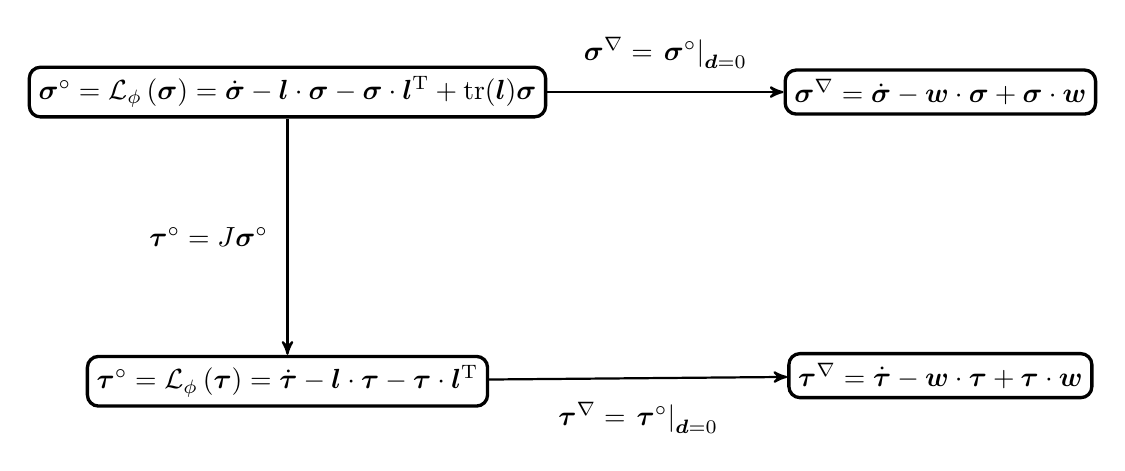
\begin{tikzpicture}[start chain=going below]
    \node [input, fill=white] (sigT) {$\ten{\sigma}^{\circ} = \mathcal{L}_{\phi} \left( \ten{\sigma} \right) = \dot{\ten{\sigma}} -  \ten{l} \cdot \ten{\sigma} -  \ten{\sigma} \cdot \ten{l} ^{\scas{T}} + \mbox{tr} (\ten{l}) \ten{\sigma} $ };
    \node [input, fill=white, right=3cm of sigT] (sigJ) {$\ten{\sigma}^{\nabla} = \dot{\ten{\sigma}} - \ten{w} \cdot \ten{\sigma} +  \ten{\sigma} \cdot \ten{w}$};
    \node [input, fill=white, below=3cm of sigJ] (tauJ) {$\ten{\tau}^{\nabla} = \dot{\ten{\tau}} - \ten{w} \cdot \ten{\tau} +  \ten{\tau} \cdot \ten{w} $};
    \node [input, fill=white, below=3cm of sigT] (tauT) {$\ten{\tau}^{\circ} = \mathcal{L}_{\phi} \left( \ten{\tau} \right) = \dot{ \ten{\tau} } -  \ten{l} \cdot \ten{\tau} - \ten{\tau} \cdot \ten{l}^{\scas{T}} $};
    \draw [lineR] (sigT) to node [yshift=0.5cm] {$\ten{\sigma}^{\nabla} = \left. \ten{\sigma}^{\circ} \right|_{\tens{d} = 0} $ } (sigJ);
    \draw [lineR] (tauT) to node [yshift=-0.5cm] {$\ten{\tau}^{\nabla} = \left. \ten{\tau}^{\circ} \right|_{\tens{d} = 0} $ } (tauJ);
    \draw [lineR] (sigT) to node [xshift=-1.0cm] {$\ten{\tau}^{\circ} = J \ten{\sigma}^{\circ} $ } (tauT);
\end{tikzpicture} \end{center}

For more information on stress rates, see Bonet \& Wood, p152, or Holzapfel, p192.  

\subsection{Tangents}
\label{subsec:tangents}
Tangents relate the change in stress (or stress rate) to the change in strain (or strain rate).

\subsubsection{Lagrangian Elasticity Tensor}
The Lagrangian elasticity tensor or tangent arises from the linearization of the stress, 
\begin{align}
D \ten{S}_{IJ} ={}& \left. \frac{\partial }{\partial \varepsilon} \left( \ten{S}_{IJ} \Big( \ten{E} (\ten{u} + \varepsilon \ten{\delta u} ) \Big) \right) \right|_{\tens{\varepsilon} = 0} 
\\
={}& \frac{ \partial \ten{S}_{IJ} }{ \partial \ten{E}_{KL} } \left. \frac{\partial }{\partial \varepsilon} \ten{E}_{KL} (\ten{u} + \varepsilon \ten{\delta u} ) \right|_{\tens{\varepsilon} = 0} 
\notag \\
={}& \frac{ \partial \ten{S}_{IJ} }{ \partial \ten{E}_{KL} }  D \ten{E}_{KL} (\ten{u} ) 
\notag \\
D \ten{S}_{IJ} ={}& \tenf{C}_{IJKL} D \ten{E}_{KL} (\ten{u} ) \, . 
\end{align}
Thus we have the Lagrangian elasticity tensor, 
\begin{equation}
\tenf{C}_{IJKL} = \frac{ \partial \ten{S}_{IJ} }{ \partial \ten{E}_{KL} } = 2 \frac{ \partial \ten{S}_{IJ} }{ \partial \ten{C}_{KL} } \, , 
\end{equation}
which has both minor symmetries but not necessarily major symmetry.  

\subsubsection{Eulerian Elasticity Tensor}
The spatial equivalent is ``intractable'' so instead the rate form is used.  (Essentially, the terms $\ten{S}$ and $\ten{E}$ can be linearized in the direction of $\ten{v}$ instead of $\ten{u}$.)  This is done using the fact that the time derivative of the second Piola-Kirchhoff stress is the pull back of the Truesdell stress rate and the time derivative of the Green-Lagrange strain tensor is the pull back of the rate of deformation,
\begin{equation}
\dot{\ten{S}}  
= \ten{F}^{-1} \cdot \ten{ \tau }^{\circ} \cdot \ten{F}^{-\scas{T}} 
= J \ten{F}^{-1} \cdot \ten{ \sigma }^{\circ} \cdot \ten{F}^{-\scas{T}}
\qquad \mbox{and} \qquad 
\dot{\ten{E}} = \ten{F}^{\scas{T}} \cdot \ten{d} \cdot \ten{F} \, .
\end{equation}
Thus, 
\begin{align}
\dot{\ten{S}}_{IJ} ={}& \tenf{C}_{IJKL} \dot{\ten{E}}_{KL}
\\
\ten{F}^{-1}_{Ii} \ten{ \tau }^{\circ}_{ij} \ten{F}^{-1}_{Jj} ={}& \tenf{C}_{IJKL} \ten{F}_{kK} \ten{d}_{kl} \ten{F}_{lL}
\notag \\
\ten{ \tau }^{\circ}_{ij} ={}& \underbrace{ \tenf{C}_{IJKL} \ten{F}_{iI} \ten{F}_{jJ} \ten{F}_{kK} \ten{F}_{lL} }_{J \tenf{c}_{ijkl}}  \ten{d}_{kl}
\notag \\
\ten{ \tau }^{\circ}_{ij} ={}& J \tenf{c}_{ijkl} \ten{d}_{kl} 
\\
\ten{ \sigma }^{\circ}_{ij} ={}& \tenf{c}_{ijkl} \ten{d}_{kl} \, ,
\end{align}
and the Eulerian elasticity tensor is defined as
\begin{equation}
\tenf{c}_{ijkl} = \frac{1}{J} \tenf{C}_{IJKL} \ten{F}_{iI} \ten{F}_{jJ} \ten{F}_{kK} \ten{F}_{lL} 
\qquad \mbox{or} \qquad
\tenf{c}  = \frac{1}{J} \big[ \ten{F} \overline{\otimes} \ten{F} \big] : \tenf{C} : \big[ \ten{F}^{\scas{T}} \overline{\otimes} \ten{F}^{\scas{T}} \big] \, , 
\end{equation}
which similarly has both minor symmetries but not necessarily major symmetry.  


\subsubsection{Jaumann Elasticity Tensor}
The objective stress rate used by Abaqus is actually the \hyperlink{jaumann}{Jaumann} stress rate instead of the Truesdell stress rate, given by: 
\begin{equation}
{C}^{\scas{Abaqus}} = \frac{1}{J} \frac{\partial \Delta \left( J \ten{\sigma} \right)}{\partial \Delta \ten{\varepsilon}}
\end{equation}

The format of the elasticity tensor can be found using the relationship between the two stress rates, 
\begin{align}
\ten{ \tau }^{\circ} ={}& J \tenf{c} : \ten{d} 
\\
\ten{\tau}^{\nabla }  - \ten{d} \cdot \ten{\tau} - \ten{\tau} \cdot \ten{d} ={}& J \tenf{c} : \ten{d} 
\notag \\
\ten{\tau}^{\nabla } ={}& J \tenf{c} : \ten{d} + \ten{d} \cdot \ten{\tau} + \ten{\tau} \cdot \ten{d} 
\notag \\
\ten{\tau}^{\nabla } ={}& J \left[ \tenf{c} : \ten{d} + \ten{d} \cdot \ten{\sigma} + \ten{\sigma} \cdot \ten{d} \right] \, .
\end{align}
We are seeking a tangent that will satisfy the equation
\begin{equation}
\ten{\tau}^{\nabla } = J \tenf{c}^\text{Abaqus} : \ten{d} \, . 
\end{equation}
That is, 
\begin{align}
J \tenf{c}^\text{Abaqus} : \ten{d} ={}& J \left[ \tenf{c} : \ten{d} + \ten{d} \cdot \ten{\sigma} + \ten{\sigma} \cdot \ten{d} \right]  
\notag \\
\tenf{c}^\text{Abaqus} : \ten{d} ={}& \tenf{c} : \ten{d} + \ten{d} \cdot \ten{\sigma} + \ten{\sigma} \cdot \ten{d}  
\notag \\
\tenf{c}^\text{Abaqus} : \ten{d} ={}& \left[ \tenf{c} + \tenf{c}' \right] : \ten{d} \, , 
\end{align}
where $\tenf{c}'$ is some fourth-order tangent that satisfies
\begin{equation}
\tenf{c}' : \ten{d}  = \ten{d} \cdot \ten{\sigma} + \ten{\sigma} \cdot \ten{d} \, . 
\end{equation}
Because the double contraction with a symmetric tensor is not unique (see Section \ref{sec:tensorderivatives} for an explanation), there are an infinite number of tensors that could satisfy this.  We restrict this further by requiring major and minor symmetries and find the form to be
\begin{align}
\tenf{c}'_{ijkl} ={}& \frac{1}{2} \left[ \delta_{ik}\sigma_{jl} + \delta_{il}\sigma_{jk} + \delta_{jk}\sigma_{il} + \delta_{jl}\sigma_{ik} \right]
\\
\tenf{c}' ={}& \frac{1}{2} \left[ \ten{I} \overline{\otimes} \ten{ \sigma}  + \ten{I} \underline{\otimes} \ten{\sigma} + \ten{\sigma} \underline{\otimes} \ten{I} + \ten{\sigma} \overline{\otimes} \ten{I} \right] 
\\
\tenf{c}' ={}& \left[ \begin{array}{cccccc}
2\sigma_1 & 0 & 0 & \sigma_4 & \sigma_5 & 0 \\
 & 2\sigma_2 & 0 & \sigma_4 & 0 & \sigma_6 \\
 &  & 2\sigma_3 & 0 & \sigma_5 & \sigma_6 \\
 &  &  & \frac{1}{2} (\sigma_1 + \sigma_2) & \frac{1}{2} \sigma_6 & \frac{1}{2} \sigma_5 \\
 & sym. &  &  & \frac{1}{2} (\sigma_1 + \sigma_3) & \frac{1}{2} \sigma_4 \\
 &  &  &  &  & \frac{1}{2} (\sigma_2 + \sigma_3)
\end{array} \right], .  
\end{align}
This extra term, the geometric tangent, can be reduced to purely kinematic terms.  Thus we have the Abaqus tangent \cite{Prot2009,Bower},
\begin{equation}
\tenf{c}^\text{Abaqus} =  \tenf{c} + \tenf{c}' \, , 
\end{equation}
which relates the volume-normalized Jaumann rate of the Kirchhoff stress to the symmetric rate of deformation tensor, 
\begin{equation}
\frac{1}{J} \ten{\tau}^{\nabla } = \tenf{c}^\text{Abaqus} : \ten{d} \, .
\end{equation}
% This can be confirmed: 
% \begin{align}
% \tenf{c}^\text{Abaqus}_{ijkl} ={}& \frac{1}{J} \frac{ \partial \ten{\tau}^{\nabla }_{ij} } { \partial \ten{d}_{kl} } 
% \\
% ={}& \frac{1}{J} \frac{ \partial \left( \ten{\tau}^{\circ}_{ij} + \ten{d}_{im} \ten{\tau}_{mj} + \ten{\tau}_{im} \ten{d}_{mj} \right) } { \partial \ten{d}_{kl} } 
% \notag \\
% ={}& \frac{1}{J} \frac{ \partial \ten{\tau}^{\circ}_{ij} } { \partial \ten{d}_{kl} } 
% + \frac{1}{J} \frac{ \partial \left( \ten{d}_{im} \ten{\tau}_{mj} \right) } { \partial \ten{d}_{kl} } 
% + \frac{1}{J} \frac{ \partial \left( \ten{\tau}_{im} \ten{d}_{mj} \right) } { \partial \ten{d}_{kl} } 
% \notag \\
% ={}& \frac{1}{J} \frac{ \partial \ten{\tau}^{\circ}_{ij} } { \partial \ten{d}_{kl} } 
% + \frac{1}{J} \frac{ \partial \ten{d}_{im} } { \partial \ten{d}_{kl} } \ten{\tau}_{mj} 
% + \ten{\tau}_{im} \frac{1}{J} \frac{ \partial \ten{d}_{mj} } { \partial \ten{d}_{kl} } 
% \notag \\
% ={}& \frac{ \partial \ten{\sigma}^{\circ}_{ij} } { \partial \ten{d}_{kl} }
% + \frac{ \partial \ten{d}_{im} } { \partial \ten{d}_{kl} } \ten{\sigma}_{mj} 
% + \ten{\sigma}_{im} \frac{ \partial \ten{d}_{mj} } { \partial \ten{d}_{kl} } 
% \notag \\
% ={}& \frac{ \partial \ten{\sigma}^{\circ}_{ij} } { \partial \ten{d}_{kl} }
% + \frac{1}{2} \left( \delta_{ik} \delta_{ml} + \delta_{il} \delta_{mk} \right) \ten{\sigma}_{mj} 
% + \frac{1}{2} \ten{\sigma}_{im} \left[ \delta_{mk} \delta_{jl} + \delta_{ml} \delta_{jk} \right] 
% \notag \\
% ={}& \frac{ \partial \ten{\sigma}^{\circ}_{ij} } { \partial \ten{d}_{kl} }
% + \frac{1}{2} \left[ \delta_{ik} \ten{\sigma}_{lj} + \delta_{il} \ten{\sigma}_{kj} \right] 
% + \frac{1}{2} \left[ \delta_{jl} \ten{\sigma}_{ik}  + \delta_{jk} \ten{\sigma}_{il}  \right] 
% \notag \\
% ={}& \frac{ \partial \ten{\sigma}^{\circ}_{ij} } { \partial \ten{d}_{kl} }
% + \frac{1}{2} \left[ \delta_{ik} \ten{\sigma}_{lj} + \delta_{il} \ten{\sigma}_{kj} + \delta_{jl} \ten{\sigma}_{ik}  + \delta_{jk} \ten{\sigma}_{il}  \right] 
% \notag \\
% \tenf{c}^\text{Abaqus}_{ijkl} ={}& \tenf{c}_{ijkl} + \frac{1}{2} \left[ \delta_{ik} \ten{\sigma}_{lj} + \delta_{il} \ten{\sigma}_{kj} + \delta_{jl} \ten{\sigma}_{ik}  + \delta_{jk} \ten{\sigma}_{il}  \right] 
% \\
% \tenf{c}^\text{Abaqus} ={}& \tenf{c} + \frac{1}{2} \left[ \ten{I} \overline{\otimes} \ten{\sigma}  + \ten{I} \underline{\otimes} \ten{\sigma}  +  \ten{\sigma} \underline{\otimes} \ten{I} + \ten{\sigma} \overline{\otimes} \ten{I} \right] 
% \end{align}



\section{Mixed Formulation}
Some calculations are performed in the spatial domain (as in Abaqus), some in the reference domain, and some in a `'mixed domain' (as in the Kuhl lab Matlab code).  The latter, the mixed domain formulation, uses the First Piola-Kirchhoff stress 
and the mixed-domain tangent, defined as
\begin{equation}
\ten{P} = \frac{ \partial W_0 }{ \partial \ten{F} }
\qquad \mbox{and} \qquad
\tenf{A} = \frac{ \partial \ten{P} }{ \partial \ten{F} }
\end{equation}
These two quantities are related to their reference counterparts by 
\begin{equation}
\ten{P} = \ten{F} \cdot \ten{S} 
\qquad \mbox{or} \qquad
\ten{P} = \ten{F}_{iI} \ten{S}_{IJ}
\end{equation}
and
\begin{equation}
\tenf{A} = \left( \ten{F} \overline{\otimes} \ten{I} \right) : \tenf{C}_{IJKL} : \left( \ten{F}^{\scas{T}} \overline{\otimes} \ten{I} \right) + \ten{I} \overline{\otimes} \ten{S} 
\qquad \mbox{or} \qquad
\tenf{A} = \ten{F}_{iI} \tenf{C}_{IJKL} \ten{F}_{kK} + \delta_{ik} \ten{S}_{JL}
\end{equation}


%%%%%%%%%%%%%%%%%%%%%%%%%%%%%%%%%%%%%%%%%%%%%%%%%%%%%%
%%%%%%%%%%%%%%%%%%%%%%%%%%%%%%%%%%%%%%%%%%%%%%%%%%%%%%
\section{Neo-Hookean Constitutive Model} 
%%%%%%%%%%%%%%%%%%%%%%%%%%%%%%%%%%%%%%%%%%%%%%%%%%%%%%
%%%%%%%%%%%%%%%%%%%%%%%%%%%%%%%%%%%%%%%%%%%%%%%%%%%%%%
Hyperelastic materials are derived from a strain energy function (or free energy function) that represents the energy density of a material as a function of strain (or temperature, etc.).  One of the simplest hyperelastic material models is the Neo-Hookean, which is well-defined for an incompressible material but has many variations in compressibility.  

\subsection{Abaqus' Neo-Hookean Constitutive Model}
Abaqus uses a different formulation of the Neo-Hookean constitutive model, 
\begin{equation}
W_0 = D_1 \left[ J - 1 \right]^2 + C_{10} \left[ \overline{I}_1 - 3 \right] \, , 
\end{equation}
with material constants  
\begin{equation}
D_1 = \frac{\kappa}{2} = \frac{1}{2} \frac{3 \lambda + 2 \mu}{3} 
\qquad \mbox{and} \qquad
C_{10} = \frac{\mu}{2} \, ,
\end{equation}
where quantities with an overbar (like $\overline{I}_1$) indicate the isochoric, or volume preserving part.  This is based on the definition of the isochoric deformation gradient,
\begin{equation}
\overline{ \ten{F} } = J^{-1/3} \ten{F} \, , 
\end{equation}
which leads to the definition of the Right Cauchy Green deformation tensor with volume change removed, 
\begin{equation}
\overline{ \ten{C} } = \overline{ \ten{F} }^{\scas{T}} \cdot \overline{ \ten{F} } = J^{-2/3} \ten{C} \, . 
\end{equation}


\subsubsection{Stress}
The Second Piola-Kirchhoff stress is derived from the free energy function, 
\begin{align}
\ten{S} ={}& 2 \frac{\partial W_0}{\partial \ten{C}}  
\\
% % begin derivations 
% ={}& 2 \frac{\partial }{\partial \ten{C}} \Big( D_1 \left[ J - 1 \right]^2 + C_{10} \left[ \overline{I}_1 - 3 \right] \Big)  
% \notag \\
% ={}& 2 D_1 \frac{\partial }{\partial \ten{C}} \left( J - 1 \right)^2 + 2 C_{10} \frac{\partial }{\partial \ten{C}} \left( \overline{I}_1 - 3 \right)  
% \notag \\
% ={}& 4 D_1 \left[ J - 1 \right] \frac{\partial J}{\partial \ten{C}} + 2 C_{10} \frac{\partial \overline{I}_1 }{\partial \ten{C}}  
% \notag \\
% ={}& 4 D_1 \left[ J - 1 \right] \frac{J}{2} \ten{C}^{-1} + 2 C_{10} \frac{\partial \overline{I}_1 }{\partial \overline{\ten{C}}} : \frac{\partial \overline{\ten{C}} }{\partial \ten{C}}  
% \notag \\
% \ten{S}_{IJ} ={}& 2 D_1 \left[ J - 1 \right] J \ten{C}^{-1}_{IJ} + 2 C_{10} \delta_{KL} : \frac{\partial \left( J^{-2/3} \ten{C}_{KL} \right) }{\partial \ten{C}_{IJ} }  
% \notag \\
% ={}& 2 D_1 \left[ J - 1 \right] J \ten{C}^{-1}_{IJ} + 2 C_{10} \delta_{KL} \left[ J^{-2/3} \frac{\partial \ten{C}_{KL} } {\partial \ten{C}_{IJ}} + \frac{\partial J^{-2/3} }{\partial J} \frac{\partial J}{\partial \ten{C}_{IJ}} \ten{C}_{KL} \right]  
% \notag \\
% ={}& 2 D_1 \left[ J - 1 \right] J \ten{C}^{-1}_{IJ} + 2 C_{10} \left[ J^{-2/3} \delta_{KL} \frac{1}{2} \left[ \delta_{KI} \delta_{LJ} + \delta_{KJ} \delta_{LI} \right) - \delta_{KL} \frac{2}{3} J^{-5/3} \frac{J}{2} \ten{C}^{-1}_{IJ} \ten{C}_{KL} \right]
% \notag \\
% ={}& 2 D_1 \left[ J - 1 \right] J \ten{C}^{-1}_{IJ} + 2 C_{10} \left[ J^{-2/3} \delta_{IJ} - \frac{1}{3} J^{-2/3} \ten{C}_{KK} \ten{C}^{-1}_{IJ} \right]
% \notag \\
% % end derivations
\cdots{}& \notag \\
\ten{S} ={}& \frac{3 \lambda + 2 \mu}{3} \left[ J - 1 \right] J \ten{C}^{-1} + \mu J^{-2/3} \left[ \ten{I} - \frac{1}{3} I_1 \ten{C}^{-1} \right] \, . 
\end{align}
This is then pushed forward into the spatial configuration to the Cauchy stress, which is the stress required by Abaqus, 
\begin{align}
\ten{\sigma} 
={}& \frac{1}{J} \ten{F} \cdot \ten{S} \cdot \ten{F}^{\scas{T}} 
\\
% % begin derivations
% ={}& \frac{1}{J} \ten{F} \cdot \left[ \frac{3 \lambda + 2 \mu}{3} \left[ J - 1 \right] J \ten{C}^{-1} + \mu J^{-2/3} \left[ \ten{I} - \frac{1}{3} I_1 \ten{C}^{-1} \right] \right] \cdot \ten{F}^{\scas{T}}  
% \notag \\
% ={}& \frac{1}{J} \left[ \frac{3 \lambda + 2 \mu}{3} \left[ J - 1 \right] J \ten{F} \cdot \ten{C}^{-1} \cdot \ten{F}^{\scas{T}} + \mu  J^{-2/3} \left[ \ten{F} \cdot \ten{I} \cdot \ten{F}^{\scas{T}} - \frac{1}{3} I_1 \ten{F} \cdot \ten{C}^{-1}\cdot \ten{F}^{\scas{T}} \right] \right]  
% \notag \\
% % end derivations
\cdots{}& \notag \\
\ten{\sigma} 
={}& \frac{3 \lambda + 2 \mu}{3} \left[ J - 1 \right] \ten{I} + \mu J^{-5/3} \left[ \ten{b} - \frac{1}{3} I_1 \ten{I} \right] \, . 
\end{align}

\subsubsection{Tangent}
The Lagrangian tangent, $\tenf{C}$, is defined as
\begin{align}
\tenf{C}_{IJKL} ={}& 2 \frac{\partial \ten{S}_{IJ} }{\partial \ten{C}_{KL} }  
\\
% % begin derivations
% ={}& 2 \frac{\partial }{\partial \ten{C}_{KL}} \left( \frac{3 \lambda + 2 \mu}{3} \left[ J - 1 \right] J \ten{C}^{-1}_{IJ} + \mu J^{-2/3} \left[ \delta_{IJ} - \frac{1}{3} I_1 \ten{C}^{-1}_{IJ} \right] \right)  
% \notag \\
% ={}& 2\frac{3 \lambda + 2 \mu}{3} \frac{\partial }{\partial \ten{C}_{KL} } \Big( \left[ J^2 - J \right) \ten{C}^{-1}_{IJ} \Big) + 2 \mu \frac{\partial }{\partial \ten{C}_{KL} } \left( J^{-2/3} \left[ \delta_{IJ} - \frac{1}{3} I_1 \ten{C}^{-1}_{IJ} \right] \right)
% \notag \\
% ={}& 2 \frac{3 \lambda + 2 \mu}{3} \left[ \frac{\partial \left( J^2 - J \right) }{\partial \ten{C}_{KL}} \ten{C}^{-1}_{IJ} + \left[ J^2 - J \right] \frac{\partial \ten{C}^{-1}_{IJ} }{\partial \ten{C}_{KL}} \right] + 2 \mu \left[ \frac{\partial J^{-2/3} }{\partial \ten{C}_{KL}} \left[ \delta_{IJ} - \frac{1}{3} I_1 \ten{C}^{-1}_{IJ} \right] - J^{-2/3} \frac{1}{3} \frac{\partial \left( I_1 \ten{C}^{-1}_{IJ} \right) }{\partial \ten{C}_{KL}} \right]  
% \notag \\ 
% ={}& 2 \frac{3 \lambda + 2 \mu}{3} \left[ \frac{\partial \left( J^2 - J \right) }{\partial J } \frac{\partial J }{\partial \ten{C}_{KL}} \ten{C}^{-1}_{IJ} - \left[ J^2 - J \right] \frac{1}{2} \left[ \ten{C}^{-1}_{IK} \ten{C}^{-1}_{JL} + \ten{C}^{-1}_{IL} \ten{C}^{-1}_{JK} \right] \right] \notag
% \\ & +  2 \mu \left[ \frac{\partial J^{-2/3} }{\partial J } \frac{\partial J }{\partial \ten{C}_{KL}} \left[ \delta_{IJ} - \frac{1}{3} I_1 \ten{C}^{-1}_{IJ} \right] - J^{-2/3} \frac{1}{3} \Bigg[ I_1 \frac{\partial \ten{C}^{-1}_{IJ} }{\partial \ten{C}_{KL}} + \frac{\partial I_1 }{\partial \ten{C}_{KL}} \ten{C}^{-1}_{IJ} \Bigg] \right]  
% \notag \\ 
% ={}& 2 \frac{3 \lambda + 2 \mu}{3} \left[ \left[ 2J - 1 \right] \frac{J}{2} \ten{C}^{-1}_{KL} \ten{C}^{-1}_{IJ} - \left[ J^2 - J \right] \frac{1}{2} \left[ \ten{C}^{-1}_{IK} \ten{C}^{-1}_{JL} + \ten{C}^{-1}_{IL} \ten{C}^{-1}_{JK} \right] \right] \notag
% \\ & +  2 \mu \left[ -\frac{2}{3} J^{-5/3} \frac{J}{2} \ten{C}^{-1}_{KL} \left[ \delta_{IJ} - \frac{1}{3} I_1 \ten{C}^{-1}_{IJ} \right] - J^{-2/3} \frac{1}{3} \Bigg[ I_1 \frac{1}{2} \left[ \ten{C}^{-1}_{IK} \ten{C}^{-1}_{JL} + \ten{C}^{-1}_{IL} \ten{C}^{-1}_{JK} \right] + \delta_{KL} \ten{C}^{-1}_{IJ} \Bigg] \right]  
% \notag \\ 
% ={}& \frac{3 \lambda + 2 \mu}{3} \Big[ \left[ 2J - 1 \right] J \ten{C}^{-1}_{IJ} \ten{C}^{-1}_{KL} - \left[ J^2 - J \right] \left[ \ten{C}^{-1}_{IK} \ten{C}^{-1}_{JL} + \ten{C}^{-1}_{IL} \ten{C}^{-1}_{JK} \right] \Big] \notag
% \\ & - 2 \mu \left[ \frac{1}{3} J^{-2/3} \ten{C}^{-1}_{KL} \delta_{IJ} - \frac{1}{9} J^{-2/3} I_1 \ten{C}^{-1}_{IJ} \ten{C}^{-1}_{KL} + J^{-2/3} \frac{1}{6} I_1 \left[ \ten{C}^{-1}_{IK} \ten{C}^{-1}_{JL} + \ten{C}^{-1}_{IL} \ten{C}^{-1}_{JK} \right] + J^{-2/3} \frac{1}{3} \delta_{KL} \ten{C}^{-1}_{IJ} \right]  
% \notag \\ 
% % end derivations
\cdots{}& \notag \\
\tenf{C}_{IJKL} ={}& \frac{3 \lambda + 2 \mu}{3} J \Big[ \left[ 2J - 1 \right] \ten{C}^{-1}_{IJ} \ten{C}^{-1}_{KL} - \left[ J - 1 \right] \left[ \ten{C}^{-1}_{IK} \ten{C}^{-1}_{JL} + \ten{C}^{-1}_{IL} \ten{C}^{-1}_{JK} \right] \Big] \notag \\ & - \frac{2}{3} \mu  J^{-2/3} \left[ \delta_{IJ} \ten{C}^{-1}_{KL} + \ten{C}^{-1}_{IJ} \delta_{KL} - I_1 \left[ \frac{1}{3} \ten{C}^{-1}_{IJ} \ten{C}^{-1}_{KL} + \frac{1}{2} \ten{C}^{-1}_{IK} \ten{C}^{-1}_{JL} + \frac{1}{2} \ten{C}^{-1}_{IL} \ten{C}^{-1}_{JK} \right] \right] \, . 
\end{align}
This is then pushed forward to the spatial domain, 
\begin{align}
\tenf{c}_{ijkl} ={}& \frac{1}{J} \tenf{C}_{IJKL} \ten{F}_{iI} \ten{F}_{jJ} \ten{F}_{kK} \ten{F}_{lL}  
\\
% % begin derivations
% ={}& \frac{1}{J} \frac{3 \lambda + 2 \mu}{3} J \Big[ \left[ 2J - 1 \right] \ten{C}^{-1}_{IJ} \ten{C}^{-1}_{KL} - \left[ J - 1 \right] \left[ \ten{C}^{-1}_{IK} \ten{C}^{-1}_{JL} + \ten{C}^{-1}_{IL} \ten{C}^{-1}_{JK} \right] \Big] \ten{F}_{iI} \ten{F}_{jJ} \ten{F}_{kK} \ten{F}_{lL} \notag
% \\ & - \frac{1}{J} \frac{2}{3} \mu J^{-2/3} \left[ \delta_{IJ} \ten{C}^{-1}_{KL} + \ten{C}^{-1}_{IJ} \delta_{KL} - I_1 \left[ \frac{1}{3} \ten{C}^{-1}_{IJ} \ten{C}^{-1}_{KL} + \frac{1}{2} \ten{C}^{-1}_{IK} \ten{C}^{-1}_{JL} + \frac{1}{2} \ten{C}^{-1}_{IL} \ten{C}^{-1}_{JK} \right] \right] \ten{F}_{iI} \ten{F}_{jJ} \ten{F}_{kK} \ten{F}_{lL}  
% \notag \\
% ={}& \frac{3 \lambda + 2 \mu}{3} \Big[ \left[ 2J - 1 \right] \ten{F}^{-1}_{Im} \ten{F}^{-1}_{Jm} \ten{F}^{-1}_{Kn} \ten{F}^{-1}_{Ln} - \left[ J - 1 \right] \left[ \ten{F}^{-1}_{Im} \ten{F}^{-1}_{Km}  \ten{F}^{-1}_{Jn} \ten{F}^{-1}_{Ln}  + \ten{F}^{-1}_{Im} \ten{F}^{-1}_{Lm}  \ten{F}^{-1}_{Jn} \ten{F}^{-1}_{Kn} \right] \Big] \ten{F}_{iI} \ten{F}_{jJ} \ten{F}_{kK} \ten{F}_{lL} \notag
% \\ & - \frac{2}{3} \mu J^{-5/3} \left[ \delta_{IJ} \ten{F}^{-1}_{Km} \ten{F}^{-1}_{Lm} + \ten{F}^{-1}_{Im} \ten{F}^{-1}_{Jm} \delta_{KL} - I_1 \left[ \frac{1}{3} \ten{F}^{-1}_{Im} \ten{F}^{-1}_{Jm} \ten{F}^{-1}_{Kn} \ten{F}^{-1}_{Ln}  + \frac{1}{2} \ten{F}^{-1}_{Im} \ten{F}^{-1}_{Km} \ten{F}^{-1}_{Jn} \ten{F}^{-1}_{Ln} + \frac{1}{2} \ten{F}^{-1}_{Im} \ten{F}^{-1}_{Lm} \ten{F}^{-1}_{Jn} \ten{F}^{-1}_{Kn}  \right] \right] \ten{F}_{iI} \ten{F}_{jJ} \ten{F}_{kK} \ten{F}_{lL}  
% \notag \\
% ={}& \frac{3 \lambda + 2 \mu}{3} \Big[ \left[ 2J - 1 \right] \delta_{im} \delta_{jm} \delta_{kn} \delta_{ln} - \left[ J - 1 \right] \left[ \delta_{im} \delta_{km} \delta_{jn} \delta_{ln}  + \delta_{im} \delta_{lm} \delta_{jn} \delta_{kn} \right] \Big] \notag
% \\ & - \frac{2}{3} \mu J^{-5/3} \left[ \delta_{IJ} \ten{F}_{iI} \ten{F}_{jJ} \delta_{km} \delta_{lm} + \delta_{im} \delta_{jm} \ten{F}_{kK} \ten{F}_{lL} \delta_{KL} - I_1 \left[ \frac{1}{3} \delta_{im} \delta_{jm} \delta_{kn} \delta_{ln} + \frac{1}{2} \delta_{im} \delta_{km} \delta_{jn} \delta_{ln} + \frac{1}{2} \delta_{im} \delta_{lm} \delta_{jn} \delta_{kn} \right] \right]  
% \notag \\
% % end derivations
\cdots{}& \notag \\
\tenf{c}_{ijkl} ={}& \frac{3 \lambda + 2 \mu}{3} \Big[ \left[ 2J - 1 \right] \delta_{ij} \delta_{kl} - 2 \left[ J - 1 \right] \tenf{I}_{ijkl} \Big] - \frac{2}{3} \mu J^{-5/3} \left[ \ten{b}_{ij} \delta_{kl} + \delta_{ij} \ten{b}_{kl} - I_1 \left[ \frac{1}{3} \delta_{ij} \delta_{kl} + \tenf{I}_{ijkl} \right] \right]  
\\
\tenf{c}_{ijkl} ={}& \left[ \kappa \left[ 2J - 1 \right] + \frac{2}{9} \mu I_1 J^{-5/3} \right] \delta_{ij} \delta_{kl} + \left[ \frac{2}{3} \mu I_1 J^{-5/3}  - 2 \kappa \left[ J - 1 \right] \right] \tenf{I}_{ijkl} - \frac{2}{3} \mu J^{-5/3} \Big[ \ten{b}_{ij} \delta_{kl} + \delta_{ij} \ten{b}_{kl} \Big] \, . 
\end{align}
The tangent required by Abaqus is
\begin{equation}
\tenf{c}^{\scas{Abaqus}} = \tenf{c} + \tenf{c}' \, , 
\end{equation}
where the geometric tangent can be reduced to purely kinematic terms, as 
\begin{equation}
\tenf{c}'_{ijkl} = \left[ 2 \kappa (J-1) - \frac{2}{3} \mu I_1 J^{- \frac{5}{3} } \right] \tenf{I}_{ijkl} + \frac{1}{2}\mu J^{- \frac{5}{3} } \Big[ \delta_{ik} \ten{b}_{jl} + \delta_{il} \ten{b}_{jk} + \ten{b}_{il} \delta_{jk} + \ten{b}_{ik} \delta_{jl} \Big] \, . 
\end{equation}
Thus the total tangent is
\begin{equation}
\tenf{c}^{\scas{Abaqus}}_{ijkl} = \left[ \kappa \left[ 2J - 1 \right] + \frac{2}{9} \mu I_1 J^{-5/3} \right] \delta_{ij} \delta_{kl} +\mu J^{-5/3} \left[ \frac{1}{2} \delta_{ik} \ten{b}_{jl} + \frac{1}{2} \delta_{il} \ten{b}_{jk} + \frac{1}{2} \ten{b}_{il} \delta_{jk} + \frac{1}{2} \ten{b}_{ik} \delta_{jl} - \frac{2}{3} \ten{b}_{ij} \delta_{kl} - \frac{2}{3} \delta_{ij} \ten{b}_{kl} \right] \, . 
\end{equation}


\subsection{Alternate Neo-Hookean Formulations}
We most commonly use a different Neo-Hookean model, 
\begin{equation}
W_0 = \frac{\lambda}{2} \ln^2 J + \frac{\mu}{2} \left[ I_1 - 3 - 2 \ln J \right] \, ,
\end{equation}
where $\lambda$ is the Lamé constant and $\mu$ is the shear modulus.

The Cauchy stress is derived through the definition of the Second Piola-Kirchoff stress,
\begin{align}
\ten{S} ={}& 2 \frac{\partial W_0}{\partial \ten{C}}  
\\
% % begin derivations
% ={}& 2 \frac{\partial W_0}{\partial \ln J} \frac{\partial \ln J}{\partial \ten{C}} + 2 \frac{\partial W_0}{\partial I_1} \frac{\partial I_1 }{\partial \ten{C}} 
% \notag \\
% ={}& 2 \left[ \lambda \ln J - \mu \right] \left[ \frac{1}{2} \ten{C}^{-1} \right] + 2 \frac{\mu}{2} \ten{I} 
% \notag \\
% % end derivations
\cdots{}& \notag \\
\ten{S} ={}& \left[ \lambda \ln J - \mu \right] \ten{C}^{-1} + \mu \ten{I} \, , 
\end{align}
where $W_0$ is the free energy function.  This is then pushed forward into the spatial configuration to the Cauchy stress as required by Abaqus, 
\begin{align}
\ten{\sigma} ={}& \frac{1}{J} \ten{F} \cdot \ten{S} \cdot \ten{F}^{\scas{T}} 
\\
% % begin derivations 
% ={}& \frac{1}{J} \ten{F} \cdot \Big[ \left[ \lambda \ln J - \mu \right] \ten{C}^{-1} + \mu \ten{I} \Big] \cdot \ten{F}^{\scas{T}} 
% \notag \\
% ={}& \frac{1}{J} \Big[ \left[ \lambda \ln J - \mu \right] \ten{F} \cdot \ten{C}^{-1} \cdot \ten{F}^{\scas{T}} + \mu \ten{F} \cdot \ten{I} \cdot \ten{F}^{\scas{T}} \Big] 
% \notag \\
% % end derivations
\cdots{}& \notag \\
\ten{\sigma} ={}& \frac{1}{J} \Big[ \left[ \lambda \ln J - \mu \right] \ten{I} + \mu \ten{b} \Big] \, . 
\end{align}

The Lagrangian tangent, $\tenf{C}$, is defined as
\begin{align}
\tenf{C}_{IJKL} ={}& 2 \frac{\partial \ten{S}_{IJ} }{\partial \ten{C}_{KL} }  
\\
% % begin derivations
% ={}& \frac{\partial \ten{S}_{IJ} }{\partial \ln J } \frac{\partial \ln J }{\partial \ten{C}_{KL} } + \frac{\partial \ten{S}_{IJ} }{\partial \ten{C}^{-1}_{MN} } \frac{\partial \ten{C}^{-1}_{MN} }{\partial \ten{C}_{KL} }  
% \notag \\
% % should have some extra step in here if showing complete work, due to the two symmetric tensor derivatives
% ={}& 2 \lambda \ten{C}^{-1}_{IJ} \frac{1}{2} \ten{C}^{-1}_{KL}  + 2 \left[ \lambda \ln J - \mu \right] \frac{\partial \ten{C}^{-1}_{IJ} }{\partial \ten{C}_{KL} } 
% \notag \\
% % end derivations
\cdots{}& \notag \\
\tenf{C}_{IJKL} ={}& \lambda \ten{C}^{-1}_{IJ} \ten{C}^{-1}_{KL} - \left[ \lambda \ln J - \mu \right] \left[ \ten{C}^{-1}_{IK} \ten{C}^{-1}_{JL} + \ten{C}^{-1}_{IL} \ten{C}^{-1}_{JK} \right]  \, . 
\end{align}
This is then pushed forward to the spatial domain, 
\begin{align}
\tenf{c}_{ijkl} ={}& \frac{1}{J} \tenf{C}_{IJKL} \ten{F}_{iI} \ten{F}_{jJ} \ten{F}_{kK} \ten{F}_{lL} 
\\
\tenf{c}_{ijkl} ={}& \frac{1}{J} \Big[ \lambda \delta_{ij} \delta_{kl} - 2 \left[ \lambda \ln J - \mu \right] \tenf{I}_{ijkl} \Big] \, , 
\end{align}
where $\tenf{I}$ is the fourth-order symmetric identity tensor,
\begin{equation}
\tenf{I} 
= \frac{1}{2} \left[ \ten{I} \overline{\otimes} \ten{I} + \ten{I} \underline{\otimes} \ten{I} \right] 
= \mathtt{IIII} 
= \left[ \begin{array}{cccccc}
1 & 0 & 0 & 0   & 0   & 0 \\
0 & 1 & 0 & 0   & 0   & 0 \\
0 & 0 & 1 & 0   & 0   & 0 \\
0 & 0 & 0 & 0.5 & 0   & 0 \\
0 & 0 & 0 & 0   & 0.5 & 0 \\
0 & 0 & 0 & 0   & 0   & 0.5 \\
\end{array} \right] \, . 
\end{equation}
The tangent required by Abaqus is
\begin{equation}
\tenf{c}^{\scas{Abaqus}} = \tenf{c} + \tenf{c}' \, , 
\end{equation}
where the geometric tangent can be reduced to purely kinematic terms, 
\begin{equation}
\tenf{c}'_{ijkl} = \frac{2}{J} \left[ \lambda \ln J - \mu \right] \tenf{I}_{ijkl} + \frac{\mu}{2 J} \left[ \delta_{ik} \ten{b}_{jl} + \delta_{il} \ten{b}_{jk} + \ten{b}_{il} \delta_{jk} + \ten{b}_{ik} \delta_{jl} \right] \, . 
\end{equation}
Thus the total tangent is
\begin{equation}
\tenf{c}^{\scas{Abaqus}}_{ijkl} = \frac{\lambda}{J} \delta_{ij} \otimes \delta_{kl} + \frac{\mu}{2 J} \left[ \delta_{ik} \ten{b}_{jl} + \delta_{il} \ten{b}_{jk} + \ten{b}_{il} \delta_{jk} + \ten{b}_{ik} \delta_{jl} \right] \, . 
\end{equation}



%%%%%%%%%%%%%%%%%%%%%%%%%%%%%%%%%%%%%%%%%%%%%%%%%%%%%%
%%%%%%%%%%%%%%%%%%%%%%%%%%%%%%%%%%%%%%%%%%%%%%%%%%%%%%
\chapter{Mechanics of Growth}
\label{chap:mechofgrowth}
%%%%%%%%%%%%%%%%%%%%%%%%%%%%%%%%%%%%%%%%%%%%%%%%%%%%%%
%%%%%%%%%%%%%%%%%%%%%%%%%%%%%%%%%%%%%%%%%%%%%%%%%%%%%%
Growth arises from the addition mass in an open system; its opposite, shrinking, consists of the removal of mass.  These two phenomena are conceptually very similar and for the purposes of this document will both be considered to fall under the umbrella term `growth'.  This added or lost mass manifests itself in a corresponding increase or decrease in density, volume, or some combination of both.  
In this section, I lay out the basis of the theory of finite growth as generally applied to soft tissues such as the brain.  The fundamental assumptions of this theory are that i) soft tissues grow via a change in volume, in which ii) the added or removed material has the same density and other properties as the original tissue, and iii) homogeneous, unconstrained growth does not induce stress.

\section{The Three Configurations of Growth}
The motion $\chi ( \ten{X} ) = \ten{x}$, relates the location of point $\ten{X}$ in the reference (also known as the undeformed or material) configuration to its location in some deformed (also known as spatial) configuration, $\ten{x}$.  The deformation gradient, $\ten{F} = \partial \chi ( \ten{X} ) / \partial \ten{X}$, relates undeformed and deformed vectors, $d \ten{X}$ and $d \ten{x}$, respectively.  In its role as a bridge between the two configurations, it is known as a two-point tensor, with a `leg' in both the material and spatial configurations.  This is evidenced by its indices, $F_{iJ}$, where by convention the spatial domain is characterized by lower-case letters and the material by capital letters.

The general formulation for finite volumetric growth relies on the multiplicative decomposition of the deformation gradient \cite{Rodriguez1994} into an irreversible growth part and a reversible elastic part, $\ten{F} = \ten{F}^{\scas{e}} \cdot \ten{F}^{\scas{g}}$ (Fig. \ref{fig_configurations_growth}).  The growth part, $\ten{F}^{\scas{g}}$, relates the reference configuration with a fictitious intermediate, or grown, configuration, which is stress-free but may be incompatible (containing gaps or overlaps).  The elastic part, $\ten{F}^{\scas{e}}$, transforms the intermediate configuration into the fully deformed configuration and, in the process of ensuring compatibility, induces stress.  

Following the established convention for the reference and deformed configurations, we similarly indicate quantities in the intermediate configuration by a bar, as in $\overline{\ten{X}}$.  
Both the growth and elastic deformation tensors are also two-leg tensors, relating two different configurations.  We could similarly characterize indices in the intermediate configuration with a bar, such that 
\begin{equation}
F_{iK} = F^{\scas{e}}_{i\overline{J}} F^{\scas{g}}_{\overline{J} K} \, .
\end{equation}
However, in this document we confine ourselves to diagonal, and thus symmetric, growth tensors, such that the growth deformation preserves the directions (but not the lengths) of the basis vectors from the reference configuration.  Thus, the indices in the reference configuration can be used interchangeably in the grown configuration and, ommitting subscripts with a bar for simplicity, capital indices can be used for the intermediate configuration instead, such that
\begin{equation}
F_{iK} = F^{\scas{e}}_{iJ} F^{\scas{g}}_{JK} \, .  
\end{equation}

%%%%%%%%%%%%%%%%%%%%%%%%%%%%%%%%%%%%%%%%%%%%%%%%%%%%%%%%%%%%%%%%%%%
\begin{figure}[ht!]
\setlength{\unitlength}{1.0cm}
\begin{center}
\begin{picture}(10.0,7.75)
\put( 0.00, -0.25){\includegraphics*[width=10.0cm,angle=0]{figure_configurations_growth}}
\put( 1.50,  6.00){$\ten{X}$}
\put( 0.90,  5.50){$M_0, V_0, \varrho_0$}
\put( 8.15,  6.00){$\ten{x}$}
\put( 7.75,  5.50){$m, v, \rho$}
\put( 5.00,  1.00){$\overline{\ten{X}}$}
\put( 4.35,  0.50){$\overline{M}, \overline{V}, \overline{\rho}$}
\end{picture}
\end{center}
\caption[Reference, intermediate grown, and final configurations.]
{Schematic of reference, intermediate, and final configurations in the presence of growth.  Growth results in a fictitious, potentially incompatible intermediate configuration, related to the final configuration by an elastic deformation that induces stress.}
\label{fig_configurations_growth}
\end{figure}
%%%%%%%%%%%%%%%%%%%%%%%%%%%%%%%%%%%%%%%%%%%%%%%%%%%%%%%%%%%%%%%%%%%

\subsection{Mass, Volume, and Density}
Because growth involves the addition of mass, the relationships between mass, volume, and density in the three configurations are not straightforward.  In the theory of finite growth, we rely on the fundamental assumption that the added material has the same intrinsic properties as the original material \cite{Rodriguez1994}.  This means that 
the density of initial mass per unit volume in the reference configuration, $\varrho_0$, and
the density of grown mass per unit volume in the intermediate configuration, $\overline{\rho}$,
are equal to each other and do not change with time, or  
\begin{equation}
\varrho_0 = \frac{\sca{d} M_0}{\sca{d} V_0} = \frac{\sca{d} J^{\scas{g}} M_0}{\sca{d} J^{\scas{g}} V_0} = \frac{\sca{d} \overline{M}}{\sca{d} \overline{V}} = \overline{\rho} \, .
\end{equation}
However, the density of grown mass per unit volume in the reference configuration, $\rho_0$, does change with growth,
\begin{equation}
\rho_0 = \frac{ \sca{d} \overline{M} }{ \sca{d} V_0 } = \frac{ J^{\scas{g}} \, \sca{d} M_0 }{ \sca{d} V_0 } = J^{\scas{g}} \, \varrho_0 \, .
\end{equation}
Incompressibility imposes a constraint of no volume change on the elastic deformation, that is, $\det (\ten{F}^{\scas{e}}) = 1$.  Numerically, incompressibility can be formulated exactly with a Lagrange multiplier or approximately with a penalty method \cite{Hughes}.  In the penalty method, the bulk stiffness is chosen to be significantly higher than the shear stiffness ($K >> \mu$ or $\lambda >> \mu$, where $K$ is the bulk modulus, $\lambda$ is Lam\'{e}'s first constant, and $\mu$ is the shear modulus).  
For compressible materials, loading may also change the density of grown mass per unit volume in the current configuration, $\rho$,
\begin{equation}
\rho = \frac{ \sca{d} \overline{M} }{ \sca{d} V } = \frac{ J^{\scas{g}} \, \sca{d} M_0 }{ J \, \sca{d} V_0 } = \frac{1}{J^{\scas{e}}} \, \varrho_0 \, .
\end{equation}

\subsection{Strain Energy Density}
The strain energy density is generally defined per unit mass, $\psi_0$, or per unit volume, $W_0 = \varrho_0 \psi_0$, such that the total energy of the system $E$ is the integral of strain energy density over the reference mass or volume, 
\begin{equation}
E = \int_{M_0} \psi_0 ( \ten{C}, \vartheta^{\scas{g}} ) \sca{d}M_0 = \int_{V_0} W_0 ( \ten{C}, \vartheta^{\scas{g}} ) \sca{d}V_0 \, , 
\end{equation}
where the strain energy densities are functions of both the overall deformation and the amount of growth, via 
the right Cauchy-Green deformation tensor $\ten{C} = \ten{F}^{\scas{T}} \cdot \ten{F}$, and
the growth variable $\vartheta^{\scas{g}} = \det \ten{F}^{\scas{g}}$, a scalar denoting the volume change due to growth.  
In a closed system, the distinction between reference and final mass is not generally important because mass is conserved, neither entering nor exiting the system.  In an open system, however, mass (and volume) are added, along with energy.  The strain energy density as determined by mechanical testing is then actually defined per unit \textit{grown} mass or volume, $\overline{\psi}$ or $\overline{W}$ \cite{Ganghoffer2013}.  Strain energy density per initial mass and volume are related to their grown counterparts by 
\begin{align}
E ={}& \int_{\overline{M}} \overline{\psi} \sca{d}\overline{M} = \int_{M_0} \overline{\psi} J^{\scas{g}} \sca{d}M_0 = \int_{M_0} \psi_0 \sca{d}M_0 
\\ \mbox{and} \quad 
E ={}& \int_{\overline{V}} \overline{W} \sca{d}\overline{V} = \int_{V_0} \overline{W} J^{\scas{g}} \sca{d}V_0 = \int_{V_0} W_0 \sca{d}V_0 \, , 
\end{align}
where 
\begin{equation}
\psi_0 = J^{\scas{g}} \overline{\psi} \qquad \mbox{and} \qquad W_0 = J^{\scas{g}} \overline{W} \, . 
\end{equation}
It is easy to see that, in the absence of growth, $J^{\scas{g}} = 1$ and the two energy densities are equivalent ($\psi_0 = \overline{\psi}$, $W_0 = \overline{W}$).  However, without careful accounting, an increase in volume due to growth is incorrectly interpreted as a spreading out of the same amount of energy over a larger volume. 


\subsection{Pushing Forward and Pulling Back}
`Pushing forward' is an operation that converts a quantity from the reference to the deformed configuration, while `pulling back' is its opposite - an operation that reverts a quantity from the deformed to the reference configuration.  As shown in the figure above, the push forward generally uses the deformation gradient; to pull back, then, it is intuitive that the inverse of the deformation gradient is used.  

Push forwards and pull backs are also used to move between the three configurations of a growing material.  Thus, $\ten{F}^{\scas{g}}$ is used to move from the reference to the intermediate configuration, $\ten{F}^{\scas{e}}$ is used to move from the intermediate to deformed configurations, and their inverses are then used to move in the opposite direction. 

Note: this is a general rule of thumb or quick check, but is not intended as a formula.  Exact forms of the push forward and pull back must be derived for each quantity.


\section{Mechanical Representation of Biological Growth}
In order to model the mechanics of biological growth, several choices must be made based on knowledge of the underlying biology.  These include both the kinematic and kinetic parameters of growth.  

\subsection{Growth Kinematics}

The shape of the growth tensor $\ten{F}^{\scas{g}}$ describes how growth takes place, whether volume is added preferentially in a single direction, in a plane, isotropically, or in some other way. Common growth tensor options include isotropic and transversely isotropic growth.  

For isotropic growth, the growth tensor is
\begin{equation}
\ten{F}^{\scas{g}}_{\scas{iso}} = \vartheta^{\scas{g}^{1/3}} \ten{I} 
\, , \mbox{  with inverse  } \, 
\ten{F}^{\scas{g}-1}_{\scas{iso}} = \frac{1}{\vartheta^{\scas{g}^{1/3}}} \ten{I} \, .
\label{Fg_iso}
\end{equation}
Note the one-third power on the growth variable; this is introduced to preserve the physical meaning of the growth variable as the amount of mass change, manifested as volume change, $\vartheta^{\scas{g}} = \det J^{\scas{g}}$.

For transversely isotropic growth in the plane normal to $\ten{n}$, the growth tensor is
\begin{equation}
\ten{F}^{\scas{g}}_{\scas{area}} = \sqrt{\vartheta^{\scas{g}}} \ten{I} + \left[ 1 - \sqrt{\vartheta^{\scas{g}}} \right] \ten{n}^0 \otimes \ten{n}^0
\, , \mbox{  with inverse  } \, 
\ten{F}^{\scas{g}-1}_{\scas{area}} = \frac{1}{\sqrt{\vartheta^{\scas{g}}} } \ten{I} + \left[ \frac{\sqrt{\vartheta^{\scas{g}}}  - 1}{\sqrt{\vartheta^{\scas{g}}} } \right] \ten{n}^0 \otimes \ten{n}^0 \, .
\label{Fg_area}
\end{equation}

For transversely isotropic growth in the direction of $\ten{n}$, the growth tensor is
\begin{equation}
\ten{F}^{\scas{g}}_{\scas{fiber}} = \ten{I} + \left[ \vartheta^{\scas{g}} - 1 \right] \ten{n}^0 \otimes \ten{n}^0
\, , \mbox{  with inverse  } \, 
\ten{F}^{\scas{g}-1}_{\scas{fiber}} = \ten{I} + \left[ \frac{1 - \vartheta^{\scas{g}}}{\vartheta^{\scas{g}}} \right] \ten{n}^0 \otimes \ten{n}^0 \, .
\label{Fg_fiber} 
\end{equation}
Preferred directions for anisotropically growing materials are defined by unit vectors in the undeformed configuration, such as the normal vector $\ten{n}^0$.  The deformed normal $\ten{n}$ is calculated from the undeformed normal and the deformation gradient,
\begin{equation}
\ten{n} = \ten{F} \cdot \ten{n}^0 \, . 
\end{equation}
For convenience, rank-one structural tensors of the undeformed and deformed elastic normals are also calculated, 
\begin{equation}
\ten{N}^0 = \ten{n}^0 \otimes \ten{n}^0 
\qquad \mbox{and} \qquad 
\ten{N} = \ten{n} \otimes \ten{n} \, .
\end{equation}
Properties of these structural tensors, formed by the dyadic of two unit vectors, include
\begin{equation}
\mbox{tr} (\ten{N}^0) = 1 \, , \qquad
\ten{N}^0 \cdot \ten{N}^0 = \ten{N}^0 \, , \qquad \mbox{and} \qquad
\ten{N}^0 : \ten{N}^0 = 1 \, .
\end{equation}


\subsection{Growth Kinetics}
Biological growth can be generally divided into morphogen-driven, or morphogenetic, growth, and mechanically-driven growth.  In morphogenetic growth, growth is caused by signaling molecules or `morphogens' \cite{Taber1995}.  This is represented mathematically by an evolution equation for the growth without mechanical dependencies, such as
$\dot{\vartheta}^{\scas{g}} = f(t)$ or $\vartheta^{\scas{g}} = f(c)$ , 
where $t$ is the time, $c$ is some concentration, and $\dot{x}$ denotes the time derivative of a quantity $x$.  

Stretch- and stress-driven growth, unlike morphogenetic growth, have mechanical causes.  They are represented mathematically by an evolution equation, which dictates the growth rate in response to a certain mechanical stimulus.  The evolution equation is divided into two parts: the growth rate $k^{\scas{g}}$, and the growth criterion function $\phi^{\scas{g}}$,
\begin{equation}
\dot{\vartheta}^{\scas{g}} ( \vartheta^{\scas{g}}, \ten{\sigma}, \ten{C} ) = k^{\scas{g}} \left( \vartheta^{\scas{g}} \right) \phi^{\scas{g}} \left( \vartheta^{\scas{g}}, \ten{\sigma}, \ten{C} \right) \, . 
\end{equation}

\subsubsection{Growth Rate}
\label{subsec:rate}
The growth rate $k^{\scas{g}}$ describes how quickly the system is able to add or remove mass.  The simplest growth rate is linear, 
\begin{equation}
k^{\scas{g}} = \alpha \, 
\end{equation}
while a more complicated growth rate such as 
\begin{equation}
k^{\scas{g}} = \alpha \left[ \frac{ \vartheta^{\scas{g}}_{\scas{max}} - \vartheta^{\scas{g}} }{ \vartheta^{\scas{g}}_{\scas{max}} - 1} \right]^{\gamma} \, ,  
\end{equation}
can include a maximum allowable amount of growth.


\subsubsection{Growth Criterion}
\label{subsec:crit}
The growth criterion function $\phi^{\scas{g}}$ describes the conditions that must be satisfied for growth to take place.  
In mechanically-driven growth, the growth criterion function contains the mechanics dependency, relating the mechanical state of the system to its desired, or homeostatic, state.  Many biological systems have the property of homeostasis, in which a quantity is regulated to be nearly constant; in the case of mechanical homeostasis, the system may be driven to minimize stress or maintain constant tension.  The growth criterion function effectively serves as a penalty function such that when the system is very far from homeostatis, the growth rate increases.  
In the case of morphogen-driven growth, this may be a chemical concentration or a pseudotime at which growth will occur.  
A common growth criterion is based on a critical maximum value of stretch or stress, activating growth only when this value is exceeded
\begin{equation}
\phi^{\scas{g}} = \left\langle f \left( \ten{C}^{\scas{e}}, \ten{S}^{\scas{e}} \right) - f_{\scas{crit}} \right\rangle \, ,
\end{equation}
where Macauley brackets yield a value of $ \langle x \rangle = x $ when $ x > 0$, and $ \langle x \rangle = 0 $ when $ x < 0$.  
Other varieties include a critical minimum value, below which retraction is activated, which would result in a three-way controller \cite{Dennerll1989}.  At one extreme, for very low values of the critical minimum and very high values of the critical maximum, this results in the absence of growth.  At the other extreme, for critical minimum and maximum values that are identical, this simplifies to a linear controller, 
\begin{equation}
\phi^{\scas{g}} = f \left( \ten{C}^{\scas{e}}, \ten{S}^{\scas{e}} \right) - f_{\scas{crit}} \, ,
\end{equation}\
which results in either growth or contraction unless $f = f_{\scas{crit}}$.


\subsection{Local Newton Iteration}
\label{subsec:local_newton}
The growth evolution equations are generally nonlinear, so it is often not possible to solve directly for $\vartheta^{\scas{g}}$.  Instead, we linearize using implicit Euler discretization, 
\begin{equation}
\dot{\vartheta}^{\scas{g}} = k^{\scas{g}} \phi^{\scas{g}} \approx{} \frac{\vartheta^{\scas{g}} - \vartheta^{\scas{g}}_n }{\Delta t} \, , 
\end{equation}
and then solve the resulting equation by using a local Newton iteration to drive the residual $R$ to zero, 
\begin{equation}
R = \vartheta^{\scas{g}} - \vartheta^{\scas{g}}_n - k^{\scas{g}} \phi^{\scas{g}} \Delta t \, , 
\end{equation}
using the local tangent 
\begin{equation}
K = \frac{\partial R}{\partial \vartheta^{\scas{g}} } = 1 - \left[ \frac{\partial k^{\scas{g}}}{\partial \vartheta^{\scas{g}} } \phi^{\scas{g}} + k^{\scas{g}} \left. \frac{\partial \phi^{\scas{g}} }{\partial \vartheta^{\scas{g}} } \right|_{\tens{C}} \right] \Delta t \, . 
\end{equation}
After each iteration, the trial value is updated by
\begin{equation}
\vartheta^{\scas{g}} \leftarrow \vartheta^{\scas{g}} - R / K \, .  
\end{equation}


\section{Thermodynamics}
The Clausius-Duhem, or dissipation, inequality is an expression of the second law of thermodynamics.  In the theory of finite growth, the inequality takes the form of
\begin{equation}
\mathcal{D} = \ten{S} : \frac{1}{2} \dot{\ten{C}} - \dot{W_0} ( \ten{C}, \vartheta^{\scas{g}} ) - S_0 \geq 0 \, . 
\end{equation}
where $\ten{S}$ is the second Piola-Kirchhoff stress and $S_0$ is a source term. 
%or 
%\begin{equation}
%\mathcal{D} = \ten{\tau} : \ten{d} - \frac{d}{dt} (\rho \psi ) - S_0 \geq 0
%\end{equation}
% in the spatial configuration.
It can be evaluated 
\begin{align}
\mathcal{D} ={}& \ten{S} : \frac{1}{2} \dot{\ten{C}} - \left. \frac{ \partial W_0 ( \ten{C}, \vartheta^{\scas{g}} ) }{\partial \ten{C}} \right|_{\vartheta^{\scas{g}}} : \frac{ \partial \ten{C} }{ \partial t } - \left. \frac{\partial W_0 ( \ten{C}, \vartheta^{\scas{g}} ) }{\partial \vartheta^{\scas{g}} } \right|_{\tens{C}} \frac{ \partial \vartheta^{\scas{g}} }{ \partial t } - S_0 \geq 0 
\\
={}& \left[ \ten{S} - 2 \left. \frac{\partial W_0 }{\partial \ten{C}} \right|_{\vartheta^{\scas{g}}} \right] : \frac{1}{2} \dot{\ten{C}} - \left. \frac{\partial W_0}{\partial \ten{C}^{\scas{e}}} : \frac{\partial \ten{C}^{\scas{e}}}{\partial \ten{F}^{\scas{e}}} : \frac{\partial \ten{F}^{\scas{e}}}{\partial \ten{F}^{\scas{g}}} \right|_{\tens{C}} : \frac{ \partial \ten{F}^{\scas{g}} }{ \partial \vartheta^{\scas{g}} } \frac{ \partial \vartheta^{\scas{g}} }{ \partial t } - S_0  
\notag \\
% begin derivations
={}& \left[ \ten{S}_{IJ} - 2 \left. \frac{\partial W_0 }{\partial \ten{C}_{IJ}} \right|_{\vartheta^{\scas{g}}} \right] \frac{1}{2} \dot{\ten{C}}_{IJ} - \frac{\partial W_0}{\partial \ten{C}^{\scas{e}}_{IJ}} \frac{\partial \ten{C}^{\scas{e}}_{IJ}}{\partial \ten{F}^{\scas{e}}_{kL}} \left. \frac{\partial \ten{F}^{\scas{e}}_{kL}}{\partial \ten{F}^{\scas{g}}_{PQ}} \right|_{\tens{C}} \dot{\ten{F}}^{\scas{g}}_{PQ} - S_0  
\notag \\
={}& \left[ \ten{S}_{IJ} - 2 \left. \frac{\partial W_0 }{\partial \ten{C}_{IJ}} \right|_{\vartheta^{\scas{g}}} \right] \frac{1}{2} \dot{\ten{C}}_{IJ} - \frac{\partial W_0}{\partial \ten{C}^{\scas{e}}_{IJ}} \frac{\partial \left( \ten{F}^{\scas{e}}_{aI} \ten{F}^{\scas{e}}_{aJ} \right) }{\partial \ten{F}^{\scas{e}}_{kL}} \left. \frac{\partial ( \ten{F}_{kM} \ten{F}^{\scas{g}-1}_{ML} ) }{\partial \ten{F}^{\scas{g}}_{PQ}} \right|_{\tens{C}} \dot{\ten{F}}^{\scas{g}}_{PQ} - S_0  
\notag \\
={}& \left[ \ten{S}_{IJ} - 2 \left. \frac{\partial W_0 }{\partial \ten{C}_{IJ}} \right|_{\vartheta^{\scas{g}}} \right] \frac{1}{2} \dot{\ten{C}}_{IJ} - \frac{1}{2} \overline{\ten{S}}_{IJ} \left[ \frac{\partial \ten{F}^{\scas{e}}_{aI} }{\partial \ten{F}^{\scas{e}}_{kL}} \ten{F}^{\scas{e}}_{aJ} + \ten{F}^{\scas{e}}_{aI} \frac{\partial \ten{F}^{\scas{e}}_{aJ} }{\partial \ten{F}^{\scas{e}}_{kL}} \right] \ten{F}_{kM} \frac{\partial \ten{F}^{\scas{g}-1}_{ML} }{\partial \ten{F}^{\scas{g}}_{PQ}} \dot{\ten{F}}^{\scas{g}}_{PQ} - S_0  
\notag \\
={}& \left[ \ten{S}_{IJ} - 2 \left. \frac{\partial W_0 }{\partial \ten{C}_{IJ}} \right|_{\vartheta^{\scas{g}}} \right] \frac{1}{2} \dot{\ten{C}}_{IJ} - \frac{1}{2} \overline{\ten{S}}_{IJ} \Big[ \delta_{ak} \delta_{IL} \ten{F}^{\scas{e}}_{aJ} + \ten{F}^{\scas{e}}_{aI} \delta_{ak} \delta_{JL} \Big] \ten{F}_{kM} \Big[ - \frac{1}{2} \Big] \left[ \ten{F}^{\scas{g}-1}_{MP} \ten{F}^{\scas{g}-1}_{LQ} + \ten{F}^{\scas{g}-1}_{MQ} \ten{F}^{\scas{g}-1}_{LP} \right] \dot{\ten{F}}^{\scas{g}}_{PQ} - S_0  
\notag \\
={}& \left[ \ten{S}_{IJ} - 2 \left. \frac{\partial W_0 }{\partial \ten{C}_{IJ}} \right|_{\vartheta^{\scas{g}}} \right] \frac{1}{2} \dot{\ten{C}}_{IJ} 
+ \frac{1}{4} \left[ \delta_{IL} \overline{\ten{S}}_{IJ} \ten{F}^{\scas{e}}_{kJ} + \overline{\ten{S}}_{IJ} \ten{F}^{\scas{e}}_{kI} \delta_{JL} \right] \left[ \ten{F}_{kM} \ten{F}^{\scas{g}-1}_{MP} \ten{F}^{\scas{g}-1}_{LQ} + \ten{F}_{kM} \ten{F}^{\scas{g}-1}_{MQ} \ten{F}^{\scas{g}-1}_{LP} \right] \dot{\ten{F}}^{\scas{g}}_{PQ} - S_0  
\notag \\
={}& \left[ \ten{S}_{IJ} - 2 \left. \frac{\partial W_0 }{\partial \ten{C}_{IJ}} \right|_{\vartheta^{\scas{g}}} \right] \frac{1}{2} \dot{\ten{C}}_{IJ} 
+ \frac{1}{4} \left[ \overline{\ten{S}}_{LJ} \ten{F}^{\scas{e}}_{kJ} + \overline{\ten{S}}_{IL} \ten{F}^{\scas{e}}_{kI} \right] \left[ \ten{F}^{\scas{e}}_{kP} \ten{F}^{\scas{g}-1}_{LQ} + \ten{F}^{\scas{e}}_{kQ} \ten{F}^{\scas{g}-1}_{LP} \right] \dot{\ten{F}}^{\scas{g}}_{PQ} - S_0  
\notag \\
={}& \left[ \ten{S}_{IJ} - 2 \left. \frac{\partial W_0 }{\partial \ten{C}_{IJ}} \right|_{\vartheta^{\scas{g}}} \right] \frac{1}{2} \dot{\ten{C}}_{IJ} 
+ \frac{1}{4} \left[ \overline{\ten{S}}_{LJ} \ten{F}^{\scas{e}}_{kJ} \ten{F}^{\scas{e}}_{kP} \ten{F}^{\scas{g}-1}_{LQ} + \overline{\ten{S}}_{LJ} \ten{F}^{\scas{e}}_{kJ} \ten{F}^{\scas{e}}_{kQ} \ten{F}^{\scas{g}-1}_{LP} +  \overline{\ten{S}}_{IL} \ten{F}^{\scas{e}}_{kI} \ten{F}^{\scas{e}}_{kP} \ten{F}^{\scas{g}-1}_{LQ} + \overline{\ten{S}}_{IL} \ten{F}^{\scas{e}}_{kI} \ten{F}^{\scas{e}}_{kQ} \ten{F}^{\scas{g}-1}_{LP} \right] \dot{\ten{F}}^{\scas{g}}_{PQ} - S_0  
\notag \\
={}& \left[ \ten{S}_{IJ} - 2 \left. \frac{\partial W_0 }{\partial \ten{C}_{IJ}} \right|_{\vartheta^{\scas{g}}} \right] \frac{1}{2} \dot{\ten{C}}_{IJ} 
+ \frac{1}{4} \left[ 
\ten{C}^{\scas{e}}_{PJ} \overline{\ten{S}}_{JL} \ten{F}^{\scas{g}-1}_{LQ}   
+ \ten{F}^{\scas{g}-1}_{PL} \overline{\ten{S}}_{LJ} \ten{C}^{\scas{e}}_{JQ} 
+ \ten{C}^{\scas{e}}_{PI} \overline{\ten{S}}_{IL} \ten{F}^{\scas{g}-1}_{LQ} 
+ \ten{F}^{\scas{g}-1}_{PL} \overline{\ten{S}}_{LI} \ten{C}^{\scas{e}}_{IQ} 
\right] \dot{\ten{F}}^{\scas{g}}_{PQ} - S_0  
\notag \\
={}& \left[ \ten{S}_{IJ} - 2 \left. \frac{\partial W_0 }{\partial \ten{C}_{IJ}} \right|_{\vartheta^{\scas{g}}} \right] \frac{1}{2} \dot{\ten{C}}_{IJ} 
+ \frac{1}{4} \left[ 2 \ten{C}^{\scas{e}}_{PA} \overline{\ten{S}}_{AL} \ten{F}^{\scas{g}-1}_{LQ} + 2 \ten{F}^{\scas{g}-1}_{PL} \overline{\ten{S}}_{LA} \ten{C}^{\scas{e}}_{AQ} \right] \dot{\ten{F}}^{\scas{g}}_{PQ} - S_0  
\notag \\
={}& \left[ \ten{S}_{IJ} - 2 \left. \frac{\partial W_0 }{\partial \ten{C}_{IJ}} \right|_{\vartheta^{\scas{g}}} \right] \frac{1}{2} \dot{\ten{C}}_{IJ} 
+ \frac{1}{2} \left[ \overline{\ten{M}}_{PL} \ten{F}^{\scas{g}-1}_{LQ} + \overline{\ten{M}}_{QL} \ten{F}^{\scas{g}-1}_{PL} \right] \dot{\ten{F}}^{\scas{g}}_{PQ} - S_0  
\notag \\
={}& \left[ \ten{S}_{IJ} - 2 \left. \frac{\partial W_0 }{\partial \ten{C}_{IJ}} \right|_{\vartheta^{\scas{g}}} \right] \frac{1}{2} \dot{\ten{C}}_{IJ} 
+ \frac{1}{2} \left[ \overline{\ten{M}}_{PL} \dot{\ten{F}}^{\scas{g}}_{PQ} \ten{F}^{\scas{g}-1}_{LQ} + \overline{\ten{M}}_{QL} \ten{F}^{\scas{g}-1}_{PL} \dot{\ten{F}}^{\scas{g}}_{PQ} \right] - S_0  
\notag \\
={}& \left[ \ten{S}_{IJ} - 2 \left. \frac{\partial W_0 }{\partial \ten{C}_{IJ}} \right|_{\vartheta^{\scas{g}}} \right] \frac{1}{2} \dot{\ten{C}}_{IJ} 
+ \frac{1}{2} \left[ \overline{\ten{M}}_{PL} \ten{L}^{\scas{g}}_{PL} + \overline{\ten{M}}_{QL} \ten{L}^{\scas{g}}_{QL} \right] - S_0  
\notag \\
={}& \left[ \ten{S}_{IJ} - 2 \left. \frac{\partial W_0 }{\partial \ten{C}_{IJ}} \right|_{\vartheta^{\scas{g}}} \right] \frac{1}{2} \dot{\ten{C}}_{IJ} + \overline{\ten{M}}_{LA} \ten{L}^{\scas{g}}_{AL} - S_0 
\notag \\
% % end derivations
\cdots{}& \notag \\
\mathcal{D} ={}& \left[ \ten{S} - 2 \left. \frac{\partial W_0}{\partial \ten{C}} \right|_{\vartheta^{\scas{g}}} \right] : \frac{1}{2} \dot{\ten{C}} + \overline{\ten{M}} : \ten{L}^{\scas{g}} - S_0 \geq 0 \, , 
\end{align}
yielding the definition of the second Piola-Kirchhoff stress,
\begin{equation}
\ten{S} = 2 \left. \frac{\partial W_0 ( \ten{C}, \vartheta^{\scas{g}}) }{\partial \ten{C}} \right|_{\vartheta^{\scas{g}}} \, ,
\label{SPK_ref}
\end{equation}
and revealing that the growth velocity gradient, $\ten{L}^{\scas{g}} = \dot{\ten{F}}^{\scas{g}} \cdot \ten{F}^{\scas{g}-1}$, is energy conjugate to the Mandel stress tensor in the intermediate configuration, $\overline{\ten{M}} = \ten{C}^{\scas{e}} \cdot \overline{\ten{S}} $, where $\overline{\ten{S}}$ is the second Piola-Kirchhoff stress in the intermediate configuration,
\begin{equation}
\overline{\ten{S}} = 2 \frac{ \partial \overline{W} \left( \ten{C}^{\scas{e}} \right) }{ \partial \ten{C}^{\scas{e}} } \, .
\label{SPK_int}
\end{equation}

\section{Stress}
The second Piola-Kirchhoff stress can be derived easily in either the reference (Eq. \ref{SPK_ref}) or intermediate configurations (Eq. \ref{SPK_int}) by differentiating the free energy density function of the reference or grown volumes with respect to the total or elastic component of the deformation, respectively.  Because the total, growth, and elastic deformations are mutually dependent, changing the total deformation while holding the growth deformation constant is equivalent to changing the elastic deformation.  Thus, the two second Piola-Kirchhoff stresses can be related to each other as
\begin{equation}
\ten{S} = 2 \left. \frac{\partial W_0 \left( \ten{C}, \vartheta^{\scas{g}} \right) }{\partial \ten{C}} \right|_{\vartheta^{\scas{g}}} = 2 \frac{\partial W_0 \left( \ten{C}^{\scas{e}}\right) }{\partial \ten{C}^{\scas{e}}} : \left. \frac{\partial \ten{C}^{\scas{e}}}{\partial \ten{C}} \right|_{\vartheta^{\scas{g}}} = J^{\scas{g}} \ten{F}^{\scas{g}-1} \cdot \overline{\ten{S}} \cdot \ten{F}^{\scas{g}-1} \, . 
\end{equation}
The Cauchy stress, which is used in many finite element programs, is defined as the push-forward of the Piola-Kirchhoff stress from the reference into the spatial domain.  It is related to the Piola-Kirchhoff stresses by the total or elastic deformation tensors, 
\begin{equation}
\ten{\sigma} = \frac{1}{J} \ten{F} \cdot \ten{S} \cdot \ten{F}^{\scas{T}}  
\qquad \mbox{or} \qquad   
\ten{\sigma} = \frac{1}{J^{\scas{e}}} \ten{F}^{\scas{e}} \cdot \overline{\ten{S}} \cdot \ten{F}^{\scas{eT}} \, .
\end{equation}
% \begin{align}
% \ten{\sigma} ={}& \frac{1}{J} \ten{F} \cdot \ten{S} \cdot \ten{F}^{\scas{T}} 
% \\
% ={}& \frac{1}{J} \ten{F} \cdot \left[ 2 \left. \frac{\partial W_0 ( \ten{C}^{\scas{e}}) }{\partial \ten{C}} \right|_{\vartheta^{\scas{g}}} \right] \cdot \ten{F}^{\scas{T}}  
% \notag \\
% ={}& \frac{1}{J} \ten{F} \cdot \left[ 2 \left. \frac{\partial W_0 }{\partial \ten{C}^{\scas{e}}} \right|_{\vartheta^{\scas{g}}} : \left. \frac{\partial \ten{C}^{\scas{e}}}{\partial \ten{C}} \right|_{\vartheta^{\scas{g}}} \right] \cdot \ten{F}^{\scas{T}}  
% \notag \\
% ={}& \frac{1}{J} \ten{F}_{iI} \left[ 2 \left. \frac{\partial W_0 }{\partial \ten{C}_{KL}^{\scas{e}}} \right|_{\vartheta^{\scas{g}}} \left. \frac{\partial \left( \ten{F}^{\scas{e}}_{aK} \ten{F}^{\scas{e}}_{aL} \right)}{\partial \ten{C}_{IJ}} \right|_{\vartheta^{\scas{g}}} \right] \ten{F}_{jJ}  
% \notag \\
% ={}& \frac{1}{J} \ten{F}_{iI} \left[ 2 \left. \frac{\partial W_0 }{\partial \ten{C}_{KL}^{\scas{e}}} \right|_{\vartheta^{\scas{g}}} \left. \frac{\partial \left( \ten{F}_{aM} \ten{F}^{\scas{g}-1}_{MK} \ten{F}_{aN} \ten{F}^{\scas{g}-1}_{NL} \right)}{\partial \ten{C}_{IJ}} \right|_{\vartheta^{\scas{g}}} \right] \ten{F}_{jJ}  
% \notag \\
% ={}& \frac{1}{J} \ten{F}_{iI} \left[ 2 \left. \frac{\partial W_0 }{\partial \ten{C}_{KL}^{\scas{e}}} \right|_{\vartheta^{\scas{g}}} \frac{\partial \left( \ten{F}_{aM} \ten{F}_{aN} \right)}{\partial \ten{C}_{IJ}} \ten{F}^{\scas{g}-1}_{MK} \ten{F}^{\scas{g}-1}_{NL} \right] \ten{F}_{jJ}   
% \notag \\
% ={}& \frac{1}{J} \ten{F}_{iI} \left[ 2 \left. \frac{\partial W_0 }{\partial \ten{C}_{KL}^{\scas{e}}} \right|_{\vartheta^{\scas{g}}} \frac{\partial \ten{C}_{MN} }{\partial \ten{C}_{IJ}} \ten{F}^{\scas{g}-1}_{MK} \ten{F}^{\scas{g}-1}_{NL} \right] \ten{F}_{jJ}   
% \notag \\
% ={}& \frac{1}{J} \ten{F}_{iI} \left[ 2 \left. \frac{\partial W_0 }{\partial \ten{C}_{KL}^{\scas{e}}} \right|_{\vartheta^{\scas{g}}} \right] \frac{1}{2} \left[ \delta_{MI} \delta_{NJ} + \delta_{MJ} \delta_{NI} \right] \ten{F}^{\scas{g}-1}_{MK} \ten{F}^{\scas{g}-1}_{NL} \ten{F}_{jJ}   
% \notag \\
% ={}& \frac{1}{J} \ten{F}_{iI} \left[ 2 \left. \frac{\partial W_0 }{\partial \ten{C}_{KL}^{\scas{e}}} \right|_{\vartheta^{\scas{g}}} \right] \frac{1}{2} \left[ \ten{F}^{\scas{g}-1}_{IK} \ten{F}^{\scas{g}-1}_{JL} + \ten{F}^{\scas{g}-1}_{IL} \ten{F}^{\scas{g}-1}_{JK} \right] \ten{F}_{jJ}  
% \notag \\
% ={}& \frac{1}{J} \left[ 2 \left. \frac{\partial W_0 }{\partial \ten{C}_{KL}^{\scas{e}}} \right|_{\vartheta^{\scas{g}}} \right] \frac{1}{2} \left[ \ten{F}_{iI} \ten{F}^{\scas{g}-1}_{IK} \ten{F}_{jJ} \ten{F}^{\scas{g}-1}_{JL} + \ten{F}_{iI} \ten{F}^{\scas{g}-1}_{IL} \ten{F}_{jJ} \ten{F}^{\scas{g}-1}_{JK} \right] 
% \notag \\
% ={}& \frac{1}{J} \left[ 2 \left. \frac{\partial W_0 }{\partial \ten{C}_{KL}^{\scas{e}}} \right|_{\vartheta^{\scas{g}}} \right] \frac{1}{2} \left[ \ten{F}^{\scas{e}}_{iK} \ten{F}^{\scas{e}}_{jL} + \ten{F}^{\scas{e}}_{iL} \ten{F}^{\scas{e}}_{jK} \right]
% \notag \\
% ={}& \frac{1}{2 J} \left[ \ten{F}^{\scas{e}}_{iK} \left[ 2 \left. \frac{\partial W_0 }{\partial \ten{C}_{KL}^{\scas{e}}} \right|_{\vartheta^{\scas{g}}} \right] \ten{F}^{\scas{e}}_{jL} + \ten{F}^{\scas{e}}_{iL} \left[ 2 \left. \frac{\partial W_0 }{\partial \ten{C}_{LK}^{\scas{e}}} \right|_{\vartheta^{\scas{g}}} \right] \ten{F}^{\scas{e}}_{jK} \right]  
% \notag \\
% ={}& \frac{1}{J} \ten{F}^{\scas{e}} \cdot \left[ 2 \left. \frac{\partial W_0 ( \ten{C}^{\scas{e}})}{\partial \ten{C}^{\scas{e}}} \right|_{\vartheta^{\scas{g}}} \right] \cdot \ten{F}^{\scas{eT}} \, . 
% \end{align}
Thus, for the logarithmic Neo-Hookean material model, the stresses are found to be
\begin{align}
\overline{\ten{S}} ={}& \left[ \lambda \ln J^{\scas{e}} - \mu \right] \ten{C}^{\scas{e}-1} + \mu \ten{I} 
\\
\ten{S} ={}& J^{\scas{g}} \left[ \left[ \lambda \ln J^{\scas{e}} - \mu \right] \ten{C}^{-1} + \mu \left( \ten{F}^{\scas{g}} \ten{F}^{\scas{g}} \right)^{-1} \right] 
\\
\ten{\sigma} ={}& \frac{1}{J^{\scas{e}}} \Big[ \left[ \lambda \ln J^{\scas{e}} - \mu \right] \ten{I} + \mu \ten{b}^{\scas{e}} \Big] \, . 
\end{align}


\section{Tangent}
Tangents, or elasticity tensors, relate changes in stress (or stress rate) to the changes in strain (or strain rate).  In the case of growth, stress is dependent on both the overall deformation and the amount of growth that has taken place,
$\ten{S} (\ten{C}, \vartheta^{\scas{g}}) $. Thus the total derivative becomes a partial derivative, 
\begin{equation}
\tenf{C} = 2 \frac{d \ten{S} (\ten{C}, \vartheta^{\scas{g}}) }{d \ten{C} } 
= \underbrace{ 2 \left. \frac{ \partial \ten{S} (\ten{C}, \vartheta^{\scas{g}}) }{ \partial \ten{C} } \right|_{\vartheta^{\scas{g}}} }_{ \tenf{C}^{\scas{e}} } + \underbrace{ 2 \left. \frac{\partial \ten{S} (\ten{C}, \vartheta^{\scas{g}}) }{\partial \vartheta^{\scas{g}}} \right|_{\tens{C} } \otimes \frac{ \partial \vartheta^{\scas{g}} }{ \partial \ten{C} } }_{ \tenf{C}^{\scas{g}} } \, , 
\end{equation}
revealing two terms - the elastic tangent $\tenf{C}^{\scas{e}}$, in which growth is held constant, and the growth tangent $\tenf{C}^{\scas{g}}$, in which the total deformation is held constant.  
As shown previously in Chapter \ref{chap:const}, this Lagrangian tangent must be pushed forward to produce the Eulerian equivalent, and the geometric tangent must be added to produce the tangent required by Abaqus.  


\subsection{Elastic Tangent} 
The elastic term of the tangent measures the change in stress in response to the change in total deformation, while growth remains constant, 
\begin{equation}
\tenf{C}^{\scas{e}} = 2 \left. \frac{ \partial \ten{S} ( \ten{C}, \vartheta^{\scas{g}}) }{ \partial \ten{C} } \right|_{\vartheta^{\scas{g}}} \, . 
\end{equation}
It is identical to the total tangent when growth is not included in the material model, and as it is dependent only on the free energy function, not on any characteristics of growth, it remains the same for all types of growth.  
It can be evaluated directly by writing any elastic components ($\ten{C}^{\scas{e}}, J^{\scas{e}}$) in terms of the total and growth components.  Similarly to stress, however, the Lagrangian tangent is more often derived using the chain rule
\begin{equation}
\tenf{C}^{\scas{e}} = 2 \left. \left[ \frac{ \partial \ten{S} }{ \partial \overline{\ten{S}} } : \frac{ \partial \overline{\ten{S}} }{ \partial \ten{C}^{\scas{e}} } : \frac{ \partial \ten{C}^{\scas{e} } }{ \partial \ten{C} } \right] \right|_{\vartheta^{\scas{g}}} \, .
\end{equation}
The first and third terms are easily derived to be
\begin{align}
\left. \frac{ \partial \ten{S}_{IJ} }{ \partial \overline{\ten{S}}_{MN} } \right|_{\vartheta^{\scas{g}}} 
={}& \left. \frac{ \partial \left( J^{\scas{g}} \ten{F}^{\scas{g}-1}_{IP} \overline{\ten{S}}_{PQ} \ten{F}^{\scas{g}-1}_{JQ} \right) }{ \partial \overline{\ten{S}}_{MN} } \right|_{\vartheta^{\scas{g}}}  
\\
% % begin derivations
% ={}& J^{\scas{g}} \ten{F}^{\scas{g}-1}_{IP} \left[ \frac{ \partial \overline{\ten{S}}_{PQ} }{ \partial \overline{\ten{S}}_{MN} } \right] \ten{F}^{\scas{g}-1}_{JQ}  
% \notag \\
% ={}& J^{\scas{g}} \ten{F}^{\scas{g}-1}_{IP} \frac{1}{2} \left[ \delta_{PM} \delta_{QN} + \delta_{PN} \delta_{QM} \right] \ten{F}^{\scas{g}-1}_{JQ}  
% \notag \\
% ={}& \frac{J^{\scas{g}}}{2} \left[ \ten{F}^{\scas{g}-1}_{IP} \delta_{PM} \ten{F}^{\scas{g}-1}_{JQ} \delta_{QN} + \ten{F}^{\scas{g}-1}_{IP} \delta_{PN} \ten{F}^{\scas{g}-1}_{JQ} \delta_{QM} \right]  
% \notag \\
% % end derivations
\cdots{}& \notag \\
\left. \frac{ \partial \ten{S}_{IJ} }{ \partial \overline{\ten{S}}_{MN} } \right|_{\vartheta^{\scas{g}}} 
={}& \frac{J^{\scas{g}}}{2} \left[ \ten{F}^{\scas{g}-1}_{IM} \ten{F}^{\scas{g}-1}_{JN} + \ten{F}^{\scas{g}-1}_{IN} \ten{F}^{\scas{g}-1}_{JM} \right]  
\end{align}
and
\begin{align}
\left. \frac{ \partial \ten{C}^{\scas{e}}_{PQ} }{ \partial \ten{C}_{KL} } \right|_{\vartheta^{\scas{g}}} 
={}& \left. \frac{ \partial \left( \ten{F}^{\scas{e}}_{iP} \ten{F}^{\scas{e}}_{iQ} \right) }{ \partial \ten{C}_{KL} } \right|_{\vartheta^{\scas{g}}} 
\\
% % begin derivations
% ={}& \left. \frac{ \partial ( \ten{F}_{iM} \ten{F}^{\scas{g}-1}_{MP} \ten{F}_{iN} \ten{F}^{\scas{g}-1}_{NQ} ) }{ \partial \ten{C}_{KL} } \right|_{\vartheta^{\scas{g}}} 
% \notag \\
% ={}& \ten{F}^{\scas{g}-1}_{MP} \frac{ \partial \left( \ten{F}_{iM} \ten{F}_{iN} \right) }{ \partial \ten{C}_{KL} } \ten{F}^{\scas{g}-1}_{NQ} 
% \notag \\
% ={}& \ten{F}^{\scas{g}-1}_{MP} \frac{ \partial \ten{C}_{MN} }{ \partial \ten{C}_{KL} } \ten{F}^{\scas{g}-1}_{NQ} 
% \notag \\
% ={}& \ten{F}^{\scas{g}-1}_{MP} \frac{1}{2} \left[ \delta_{MK} \delta_{NL} + \delta_{ML} \delta_{NK} \right] \ten{F}^{\scas{g}-1}_{NQ} 
% \notag \\
% % end derivations
\cdots{}& \notag \\
\left. \frac{ \partial \ten{C}^{\scas{e}}_{PQ} }{ \partial \ten{C}_{KL} } \right|_{\vartheta^{\scas{g}}} 
={}& \frac{1}{2} \left[ \ten{F}^{\scas{g}-1}_{KP} \ten{F}^{\scas{g}-1}_{LQ} 
+ \ten{F}^{\scas{g}-1}_{LP} \ten{F}^{\scas{g}-1}_{KQ} \right] 
\end{align}
while for convenience, we define the second term as the elastic tangent in the intermediate configuration,
\begin{equation}
\tenf{L}^{\scas{e}}_{MNPQ} = 2 \left. \frac{\partial \overline{\ten{S}}_{MN} }{\partial \ten{C}^{\scas{e}}_{PQ} } \right|_{\vartheta^{\scas{g}}} \, .
\end{equation}
Thus the Lagrangian elastic tangent can be rewritten in terms of the elastic tangent in the intermediate configuration,   
\begin{align}
\tenf{C}^{\scas{e}}_{IJKL} ={}& \left. \left[ \frac{ \partial \ten{S}_{IJ} }{ \partial \overline{\ten{S}}_{MN} } \, 2 \frac{ \partial \overline{\ten{S}}_{MN} }{ \partial \ten{C}^{\scas{e}}_{PQ} } \, \frac{ \partial \ten{C}^{\scas{e}}_{PQ} }{ \partial \ten{C}_{KL} } \right] \right|_{\vartheta^{\scas{g}}} 
\\
={}& \frac{J^{\scas{g}}}{2} \left[ \ten{F}^{\scas{g}-1}_{IM} \ten{F}^{\scas{g}-1}_{JN} + \ten{F}^{\scas{g}-1}_{IN} \ten{F}^{\scas{g}-1}_{JM} \right] \tenf{L}^{\scas{e}}_{MNPQ} \frac{1}{2} \left[ \ten{F}^{\scas{g}-1}_{PK} \ten{F}^{\scas{g}-1}_{QL} + \ten{F}^{\scas{g}-1}_{PL} \ten{F}^{\scas{g}-1}_{QK} \right] 
\notag \\
% % begin derivations
% ={}& \frac{J^{\scas{g}}}{4} \left[ \ten{F}^{\scas{g}-1}_{IM} \ten{F}^{\scas{g}-1}_{JN} + \ten{F}^{\scas{g}-1}_{IN} \ten{F}^{\scas{g}-1}_{JM} \right] \tenf{L}^{\scas{e}}_{MNPQ} \left[ \ten{F}^{\scas{g}-1}_{PK} \ten{F}^{\scas{g}-1}_{QL} + \ten{F}^{\scas{g}-1}_{PL} \ten{F}^{\scas{g}-1}_{QK} \right] 
% \notag \\
% ={}& \frac{J^{\scas{g}}}{4} \left[ \ten{F}^{\scas{g}-1}_{IM} \ten{F}^{\scas{g}-1}_{JN} \tenf{L}^{\scas{e}}_{MNPQ} + \ten{F}^{\scas{g}-1}_{IN} \ten{F}^{\scas{g}-1}_{JM} \tenf{L}^{\scas{e}}_{NMPQ} \right] \left[ \ten{F}^{\scas{g}-1}_{PK} \ten{F}^{\scas{g}-1}_{QL} + \ten{F}^{\scas{g}-1}_{PL} \ten{F}^{\scas{g}-1}_{QK} \right] 
% \notag \\
% % change of free indices . . .
% ={}& \frac{J^{\scas{g}}}{4} \left[ \ten{F}^{\scas{g}-1}_{IA} \ten{F}^{\scas{g}-1}_{JB} \tenf{L}^{\scas{e}}_{ABPQ} + \ten{F}^{\scas{g}-1}_{IA} \ten{F}^{\scas{g}-1}_{JB} \tenf{L}^{\scas{e}}_{ABPQ} \right] \left[ \ten{F}^{\scas{g}-1}_{PK} \ten{F}^{\scas{g}-1}_{QL} + \ten{F}^{\scas{g}-1}_{PL} \ten{F}^{\scas{g}-1}_{QK} \right] 
% \notag \\
% ={}& \frac{J^{\scas{g}}}{2} \ten{F}^{\scas{g}-1}_{IA} \ten{F}^{\scas{g}-1}_{JB} \left[ \tenf{L}^{\scas{e}}_{ABPQ} \ten{F}^{\scas{g}-1}_{PK} \ten{F}^{\scas{g}-1}_{QL} + \tenf{L}^{\scas{e}}_{ABQP} \ten{F}^{\scas{g}-1}_{PL} \ten{F}^{\scas{g}-1}_{QK} \right] 
% \notag \\
% % change of free indices . . .) 
% ={}& \frac{J^{\scas{g}}}{2} \ten{F}^{\scas{g}-1}_{IA} \ten{F}^{\scas{g}-1}_{JB} \left[ \tenf{L}^{\scas{e}}_{ABCD} \ten{F}^{\scas{g}-1}_{CK} \ten{F}^{\scas{g}-1}_{DL} + \tenf{L}^{\scas{e}}_{ABCD} \ten{F}^{\scas{g}-1}_{DL} \ten{F}^{\scas{g}-1}_{CK} \right] 
% \notag \\
% ={}& J^{\scas{g}} \ten{F}^{\scas{g}-1}_{IA} \ten{F}^{\scas{g}-1}_{JB} \tenf{L}^{\scas{e}}_{ABCD} \ten{F}^{\scas{g}-1}_{CK} \ten{F}^{\scas{g}-1}_{DL} 
% \notag \\
% % end derivations
\cdots{}& \notag \\
\tenf{C}^{\scas{e}}_{IJKL} ={}& J^{\scas{g}} \tenf{L}^{\scas{e}}_{ABCD} \ten{F}^{\scas{g}-1}_{IA} \ten{F}^{\scas{g}-1}_{JB} \ten{F}^{\scas{g}-1}_{KC} \ten{F}^{\scas{g}-1}_{LD} \, , 
\end{align}
which is obviously the pull-back from the intermediate to the reference configuration.  The Lagrangian elastic tangent $\tenf{C}^{\scas{e}}$ is then pushed forward to the spatial domain to get the Eulerian elastic tangent, 
\begin{equation}
\tenf{c}^{\scas{e}}_{ijkl} = \frac{1}{J} \tenf{C}^{\scas{e}}_{IJKL} \ten{F}_{iI} \ten{F}_{jJ} \ten{F}_{kK} \ten{F}_{lL} \, ,
\end{equation}
which is actually equivalent to pushing the intermediate elastic tangent forward directly from the intermediate configuration,
\begin{align}
\tenf{c}^{\scas{e}}_{ijkl} ={}& \frac{1}{J} \tenf{C}^{\scas{e}}_{IJKL} \ten{F}_{iI} \ten{F}_{jJ} \ten{F}_{kK} \ten{F}_{lL} \\
={}& \frac{1}{J} \left[ J^{\scas{g}} \tenf{L}^{\scas{e}}_{MNPQ} \ten{F}^{\scas{g}-1}_{IM} \ten{F}^{\scas{g}-1}_{JN} \ten{F}^{\scas{g}-1}_{KP} \ten{F}^{\scas{g}-1}_{LQ} \right] \ten{F}_{iI} \ten{F}_{jJ} \ten{F}_{kK} \ten{F}_{lL} \notag \\
={}& \frac{1}{J^{\scas{e}}} \tenf{L}^{\scas{e}}_{MNPQ} \ten{F}^{e}_{iM} \ten{F}^{e}_{jN} \ten{F}^{e}_{kP}  \ten{F}^{e}_{lQ} \, .  
\end{align}

\subsection{Growth Tangent}
\label{subsec:growth_tangent}
The growth term of the tangent measures the change in stress in response to the change in growth, while the total deformation remains constant, 
\begin{equation}
\tenf{C}^{\scas{g}} = 2 \left. \frac{\partial \ten{S} }{\partial \ten{F}^{\scas{g}} } \right|_{\tens{C}} : \frac{\partial \ten{F}^{\scas{g}} }{\partial \vartheta^{\scas{g}}} \otimes \frac{ \partial \vartheta^{\scas{g}} }{ \partial \ten{C} } \, .  
\end{equation}
It is highly dependent on both the elastic material response and the growth model.  For example, the first term is dependent on the choice of free energy function $W_0$ and growth tensor $\ten{F}^{\scas{g}}$, 
\begin{align}
2 \left. \frac{\partial \ten{S}_{IJ}}{\partial \ten{F}^{\scas{g}}_{MN}} \right|_{\tens{C}} 
={}& 2 \left. \frac{\partial \left( J^{\scas{g}} \ten{F}^{\scas{g}-1}_{IA} \overline{\ten{S}}_{AB} \ten{F}^{\scas{g}-1}_{JB} \right) }{\partial \ten{F}^{\scas{g}}_{MN}} \right|_{\tens{C}} 
\\
% % begin derivations
% ={}& 2 \left. \frac{\partial J^{\scas{g}} }{\partial \ten{F}^{\scas{g}}_{MN}} \right|_{\tens{C}} \ten{F}^{\scas{g}-1}_{IA} \overline{\ten{S}}_{AB} \ten{F}^{\scas{g}-1}_{JB} 
% + 2 J^{\scas{g}} \frac{\partial \ten{F}^{\scas{g}-1}_{IA} }{\partial \ten{F}^{\scas{g}}_{MN}} \overline{\ten{S}}_{AB} \ten{F}^{\scas{g}-1}_{JB} 
% + 2 J^{\scas{g}} \ten{F}^{\scas{g}-1}_{IA} \left. \frac{\partial \overline{\ten{S}}_{AB} }{\partial \ten{F}^{\scas{g}}_{MN}} \right|_{\tens{C}} \ten{F}^{\scas{g}-1}_{JB} 
% + 2 J^{\scas{g}} \ten{F}^{\scas{g}-1}_{IA} \overline{\ten{S}}_{AB} \frac{\partial \ten{F}^{\scas{g}-1}_{JB} }{\partial \ten{F}^{\scas{g}}_{MN}} 
% \notag \\
% ={}& 2 J^{\scas{g}} \ten{F}^{\scas{g}-1}_{NM} \ten{F}^{\scas{g}-1}_{IA} \overline{\ten{S}}_{AB} \ten{F}^{\scas{g}-1}_{JB} 
% + 2 J^{\scas{g}} \overline{\ten{S}}_{AB} \left[ \frac{\partial \ten{F}^{\scas{g}-1}_{IA} }{\partial \ten{F}^{\scas{g}}_{MN}} \ten{F}^{\scas{g}-1}_{JB} + \ten{F}^{\scas{g}-1}_{IA} \frac{\partial \ten{F}^{\scas{g}-1}_{JB} }{\partial \ten{F}^{\scas{g}}_{MN}} \right] 
% + J^{\scas{g}} \ten{F}^{\scas{g}-1}_{IA} \left[ 2 \frac{\partial \overline{\ten{S}}_{AB} }{\partial \ten{C}^{\scas{e}}_{CD}} \right] \left. \frac{\partial \ten{C}^{\scas{e}}_{CD}}{\partial \ten{F}^{\scas{g}}_{MN}} \right|_{\tens{C}} \ten{F}^{\scas{g}-1}_{JB} 
% \notag \\
% ={}& 2 J^{\scas{g}} \ten{F}^{\scas{g}-1}_{NM} \ten{F}^{\scas{g}-1}_{IA} \overline{\ten{S}}_{AB} \ten{F}^{\scas{g}-1}_{JB} 
% - J^{\scas{g}} \overline{\ten{S}}_{AB} \left[ \left[ \ten{F}^{\scas{g}-1}_{IM} \ten{F}^{\scas{g}-1}_{AN} + \ten{F}^{\scas{g}-1}_{IN} \ten{F}^{\scas{g}-1}_{AM} \right] \ten{F}^{\scas{g}-1}_{JB} + \ten{F}^{\scas{g}-1}_{IA} \left[ \ten{F}^{\scas{g}-1}_{JM} \ten{F}^{\scas{g}-1}_{BN} + \ten{F}^{\scas{g}-1}_{JN} \ten{F}^{\scas{g}-1}_{BM} \right] \right] \notag \\
% &+ J^{\scas{g}} \ten{F}^{\scas{g}-1}_{IA} \ten{F}^{\scas{g}-1}_{JB} \tenf{L}^{\scas{e}}_{ABCD} \left. \frac{ \partial \left( \ten{F}^{\scas{g}-1}_{RC} \ten{C}_{RS} \ten{F}^{\scas{g}-1}_{SD} \right) }{\partial \ten{F}^{\scas{g}}_{MN}} \right|_{\tens{C}} 
% \notag \\
% ={}& 2 \ten{F}^{\scas{g}-1}_{NM} \ten{S}_{IJ} 
% - \left[ \ten{F}^{\scas{g}-1}_{IM} \ten{S}_{NJ} + \ten{F}^{\scas{g}-1}_{IN} \ten{S}_{MJ} + \ten{F}^{\scas{g}-1}_{JM} \ten{S}_{IN} + \ten{F}^{\scas{g}-1}_{JN} \ten{S}_{IM} \right] \notag \\
% &+ J^{\scas{g}} \ten{F}^{\scas{g}-1}_{IA} \ten{F}^{\scas{g}-1}_{JB} \tenf{L}^{\scas{e}}_{ABCD} \left[ \frac{\partial \ten{F}^{\scas{g}-1}_{RC} }{\partial \ten{F}^{\scas{g}}_{MN}} \ten{C}_{RS} \ten{F}^{\scas{g}-1}_{SD} + \ten{F}^{\scas{g}-1}_{RC} \ten{C}_{RS} \frac{\partial \ten{F}^{\scas{g}-1}_{SD} }{\partial \ten{F}^{\scas{g}}_{MN}} \right]
% \notag \\
% ={}& 2 \ten{F}^{\scas{g}-1}_{NM} \ten{S}_{IJ} 
% - \ten{F}^{\scas{g}-1}_{IM} \ten{S}_{NJ} - \ten{F}^{\scas{g}-1}_{IN} \ten{S}_{MJ} - \ten{F}^{\scas{g}-1}_{JM} \ten{S}_{IN} - \ten{F}^{\scas{g}-1}_{JN} \ten{S}_{IM} \notag \\
% & - \frac{1}{2} J^{\scas{g}} \ten{F}^{\scas{g}-1}_{IA} \ten{F}^{\scas{g}-1}_{JB} \tenf{L}^{\scas{e}}_{ABCD} \left[ \left[ \ten{F}^{\scas{g}-1}_{RM} \ten{F}^{\scas{g}-1}_{CN} + \ten{F}^{\scas{g}-1}_{RN} \ten{F}^{\scas{g}-1}_{CM} \right] \ten{C}_{RS} \ten{F}^{\scas{g}-1}_{SD} + \ten{F}^{\scas{g}-1}_{RC} \ten{C}_{RS} \left[ \ten{F}^{\scas{g}-1}_{SM} \ten{F}^{\scas{g}-1}_{DN} + \ten{F}^{\scas{g}-1}_{SN} \ten{F}^{\scas{g}-1}_{DM} \right] \right]
% \notag \\
% ={}& 2 \ten{F}^{\scas{g}-1}_{NM} \ten{S}_{IJ} 
% - \ten{F}^{\scas{g}-1}_{IM} \ten{S}_{NJ} - \ten{F}^{\scas{g}-1}_{IN} \ten{S}_{MJ} - \ten{F}^{\scas{g}-1}_{JM} \ten{S}_{IN} - \ten{F}^{\scas{g}-1}_{JN} \ten{S}_{IM} \notag \\
% & - \frac{1}{2} J^{\scas{g}} \ten{F}^{\scas{g}-1}_{IA} \ten{F}^{\scas{g}-1}_{JB} \tenf{L}^{\scas{e}}_{ABCD} \left[ \ten{C}^{\scas{e}}_{MD} \ten{F}^{\scas{g}-1}_{CN} + \ten{F}^{\scas{g}-1}_{CM} \ten{C}^{\scas{e}}_{ND} + \ten{C}^{\scas{e}}_{CM} \ten{F}^{\scas{g}-1}_{DN} + \ten{F}^{\scas{g}-1}_{DM} \ten{C}^{\scas{e}}_{CN} \right]
% \notag \\
% ={}& 2 \ten{F}^{\scas{g}-1}_{NM} \ten{S}_{IJ} 
% - \ten{F}^{\scas{g}-1}_{IM} \ten{S}_{NJ} - \ten{F}^{\scas{g}-1}_{IN} \ten{S}_{MJ} - \ten{F}^{\scas{g}-1}_{JM} \ten{S}_{IN} - \ten{F}^{\scas{g}-1}_{JN} \ten{S}_{IM} \notag \\
% & - \frac{1}{2} J^{\scas{g}} \ten{F}^{\scas{g}-1}_{IA} \ten{F}^{\scas{g}-1}_{JB} \left[ \tenf{L}^{\scas{e}}_{ABDC} \ten{C}^{\scas{e}}_{DM} \ten{F}^{\scas{g}-1}_{CN} + \tenf{L}^{\scas{e}}_{ABCD} \ten{F}^{\scas{g}-1}_{CM} \ten{C}^{\scas{e}}_{DN} + \tenf{L}^{\scas{e}}_{ABCD} \ten{C}^{\scas{e}}_{CM} \ten{F}^{\scas{g}-1}_{DN} + \tenf{L}^{\scas{e}}_{ABDC} \ten{F}^{\scas{g}-1}_{DM} \ten{C}^{\scas{e}}_{CN} \right]
% \notag \\
% % change of free indices . . .   
% ={}& 2 \ten{F}^{\scas{g}-1}_{NM} \ten{S}_{IJ} 
% - \ten{F}^{\scas{g}-1}_{IM} \ten{S}_{NJ} - \ten{F}^{\scas{g}-1}_{IN} \ten{S}_{MJ} - \ten{F}^{\scas{g}-1}_{JM} \ten{S}_{IN} - \ten{F}^{\scas{g}-1}_{JN} \ten{S}_{IM} \notag \\
% & - \frac{1}{2} J^{\scas{g}} \ten{F}^{\scas{g}-1}_{IA} \ten{F}^{\scas{g}-1}_{JB} \left[ \tenf{L}^{\scas{e}}_{ABPQ} \ten{C}^{\scas{e}}_{PM} \ten{F}^{\scas{g}-1}_{QN} + \tenf{L}^{\scas{e}}_{ABPQ} \ten{F}^{\scas{g}-1}_{PM} \ten{C}^{\scas{e}}_{QN} + \tenf{L}^{\scas{e}}_{ABPQ} \ten{C}^{\scas{e}}_{PM} \ten{F}^{\scas{g}-1}_{QN} + \tenf{L}^{\scas{e}}_{ABPQ} \ten{F}^{\scas{g}-1}_{PM} \ten{C}^{\scas{e}}_{QN} \right]
% \notag \\
% % end derivations
\cdots{}& \notag \\
2 \left. \frac{\partial \ten{S}_{IJ}}{\partial \ten{F}^{\scas{g}}_{MN}} \right|_{\tens{C}} 
={}& 2 \ten{F}^{\scas{g}-1}_{NM} \ten{S}_{IJ} 
- \ten{F}^{\scas{g}-1}_{IM} \ten{S}_{NJ} - \ten{F}^{\scas{g}-1}_{IN} \ten{S}_{MJ} - \ten{F}^{\scas{g}-1}_{JM} \ten{S}_{IN} - \ten{F}^{\scas{g}-1}_{JN} \ten{S}_{IM} \notag \\
& - J^{\scas{g}} \ten{F}^{\scas{g}-1}_{IA} \ten{F}^{\scas{g}-1}_{JB} \tenf{L}^{\scas{e}}_{ABPQ} \left[ \ten{C}^{\scas{e}}_{PM} \ten{F}^{\scas{g}-1}_{QN} + \ten{F}^{\scas{g}-1}_{PM} \ten{C}^{\scas{e}}_{QN} \right] \, ,
\label{dSdFg}
\end{align}
while the second term is completely dependent on the exact form of the growth tensor $\ten{F}^{\scas{g}}$.  The last one is derived from the residual of the local Newton iteration.  For a growth evolution equation of the form 
\begin{equation}
\dot{\vartheta}^{\scas{g}} \left( \vartheta^{\scas{g}}, \ten{C}^{\scas{e}} \right) = k^{\scas{g}} \left( \vartheta^{\scas{g}} \right) \phi^{\scas{g}} \left( \vartheta^{\scas{g}}, \ten{C}^{\scas{e}} \right) \, , 
\end{equation}
the third term can be found to be
\begin{align}
\frac{\partial R^\vartheta}{\partial \ten{C}_{KL} } 
={}& \frac{\partial }{\partial \ten{C}_{KL} } \left( \vartheta^{\scas{g}} - \vartheta^{\scas{g}}_n - \dot{\vartheta}^{\scas{g}} \Delta t \right) 
\notag \\
0 
={}& \frac{\partial \vartheta^{\scas{g}} }{\partial \ten{C}_{KL} } - \frac{\partial \dot{\vartheta}^{\scas{g}} }{\partial \ten{C}_{KL} } \Delta t 
\notag \\
\frac{\partial \vartheta^{\scas{g}} }{\partial \ten{C}_{KL} } 
={}& \left[ \left. \frac{\partial \dot{\vartheta}^{\scas{g}} }{\partial \ten{C}_{KL} } \right|_{\vartheta^{\scas{g}}} + \left. \frac{\partial \dot{\vartheta}^{\scas{g}} }{\partial \vartheta^{\scas{g}}} \right|_{\tens{C}} \frac{\partial \vartheta^{\scas{g}} }{\partial \ten{C}_{KL} } \right] \Delta t 
\notag \\
\frac{\partial \vartheta^{\scas{g}} }{\partial \ten{C}_{KL} } 
={}& \left[ \left. \frac{ \partial ( k^{\scas{g}} \phi^{\scas{g}} ) }{\partial \ten{C}_{KL} } \right|_{\vartheta^{\scas{g}}} + \left. \frac{ \partial ( k^{\scas{g}} \phi^{\scas{g}} ) }{\partial \vartheta^{\scas{g}}} \right|_{\tens{C}} \frac{\partial \vartheta^{\scas{g}} }{\partial \ten{C}_{KL} } \right] \Delta t
\notag \\
\frac{\partial \vartheta^{\scas{g}} }{\partial \ten{C}_{KL} } 
={}& k^{\scas{g}} \left. \frac{ \partial \phi^{\scas{g}} }{\partial \ten{C}_{KL} } \right|_{\vartheta^{\scas{g}}} \Delta t + \left[ k^{\scas{g}} \left. \frac{ \partial \phi^{\scas{g}} }{\partial \vartheta^{\scas{g}}} \right|_{\tens{C}} + \frac{ \partial k^{\scas{g}} }{\partial \vartheta^{\scas{g}}} \phi^{\scas{g}} \right] \frac{\partial \vartheta^{\scas{g}} }{\partial \ten{C}_{KL} } \Delta t
\notag \\
\left[ 1 - \left[ k^{\scas{g}} \left. \frac{\partial \phi^{\scas{g}} }{\partial \vartheta^{\scas{g}}} \right|_{\tens{C}} + \frac{\partial k^{\scas{g}} }{\partial \vartheta^{\scas{g}}} \phi^{\scas{g}} \right] \Delta t \right] \frac{\partial \vartheta^{\scas{g}} }{\partial \ten{C}_{KL} }  
={}& k^{\scas{g}} \left. \frac{\partial \phi^{\scas{g}} }{\partial \ten{C}_{KL} } \right|_{\vartheta^{\scas{g}}} \Delta t 
\notag \\
K^\vartheta \frac{\partial \vartheta^{\scas{g}} }{\partial \ten{C}_{KL} } 
={}& k^{\scas{g}} \left. \frac{\partial \phi^{\scas{g}} }{\partial \ten{C}_{KL} ^{\scas{e}}} \right|_{\vartheta^{\scas{g}}} \Delta t 
\notag \\
\frac{\partial \vartheta^{\scas{g}} }{\partial \ten{C}_{KL} } 
={}& \frac{k^{\scas{g}} \Delta t}{K^\vartheta} \left. \frac{\partial \phi^{\scas{g}} }{\partial \ten{C}_{KL} } \right|_{\vartheta^{\scas{g}}} \, , 
\end{align}
where $\partial \phi^{\scas{g}} / \partial \ten{C}$ is obviously dependent on the choice of growth criterion, $\phi^{\scas{g}}$.  Note that the function $k^{\scas{g}}$ can be changed easily, as only its derivative $ \partial k^{\scas{g}} / \partial \vartheta^{\scas{g}}$ is needed for the local Newton iteration, while $\phi^{\scas{g}}$ appears in the tangent as $\left. \partial \phi^{\scas{g}} / \partial \ten{C}^{\scas{e}} \right|_{\vartheta^{\scas{g}}}$.

The Lagrangian growth tangent $\tenf{C}^{\scas{g}}$ is then pushed forward to the spatial domain to get the Eulerian growth tangent,
\begin{align}
\tenf{c}^{\scas{g}}_{ijkl} 
={}& \frac{1}{J} \tenf{C}^{\scas{g}}_{IJKL} \ten{F}_{iI} \ten{F}_{jJ} \ten{F}_{kK} \ten{F}_{lL} 
\\
={}& \frac{1}{J} \left[ 2 \frac{\partial \ten{S}_{IJ}}{\partial \ten{F}^{\scas{g}}_{MN}} \right] \frac{\partial \ten{F}^{\scas{g}}_{MN}}{\partial \vartheta^{\scas{g}}}  \frac{ \partial \vartheta^{\scas{g}} }{ \partial \ten{C}_{KL} } \ten{F}_{iI} \ten{F}_{jJ} \ten{F}_{kK} \ten{F}_{lL} 
\notag \\
% % begin derivations
% ={}& \frac{1}{J} \left[ 2 \ten{F}^{\scas{g}-1}_{NM} \ten{S}_{IJ} 
% - \ten{F}^{\scas{g}-1}_{IM} \ten{S}_{NJ} - \ten{F}^{\scas{g}-1}_{IN} \ten{S}_{MJ} - \ten{F}^{\scas{g}-1}_{JM} \ten{S}_{IN} - \ten{F}^{\scas{g}-1}_{JN} \ten{S}_{IM} - J^{\scas{g}} \ten{F}^{\scas{g}-1}_{IA} \ten{F}^{\scas{g}-1}_{JB} \tenf{L}^{\scas{e}}_{ABPQ} \left[ \ten{C}^{\scas{e}}_{PM} \ten{F}^{\scas{g}-1}_{QN} + \ten{F}^{\scas{g}-1}_{PM} \ten{C}^{\scas{e}}_{QN} \right] \right] \notag \\
% & \hspace{1cm} \frac{\partial \ten{F}^{\scas{g}}_{MN}}{\partial \vartheta^{\scas{g}}} \frac{k^{\scas{g}} \Delta t}{K^\vartheta} \left. \frac{\partial \phi^{\scas{g}} }{\partial \ten{C}_{KL}} \right|_{\vartheta^{\scas{g}}}  \ten{F}_{iI} \ten{F}_{jJ} \ten{F}_{kK} \ten{F}_{lL} 
% \notag \\
% ={}& \frac{1}{J} \left[ 2 \ten{F}^{\scas{g}-1}_{MN} \ten{S}_{IJ} 
% - \ten{F}^{\scas{g}-1}_{IM} \ten{S}_{NJ} - \ten{F}^{\scas{g}-1}_{IM} \ten{S}_{NJ} - \ten{F}^{\scas{g}-1}_{JN} \ten{S}_{IM} - \ten{F}^{\scas{g}-1}_{JN} \ten{S}_{IM} - J^{\scas{g}} \ten{F}^{\scas{g}-1}_{IA} \ten{F}^{\scas{g}-1}_{JB} \tenf{L}^{\scas{e}}_{ABPQ} \left[ \ten{C}^{\scas{e}}_{PM} \ten{F}^{\scas{g}-1}_{QN} + \ten{F}^{\scas{g}-1}_{PM} \ten{C}^{\scas{e}}_{QN} \right] \right] \notag \\
% & \hspace{1cm} \frac{\partial \ten{F}^{\scas{g}}_{MN}}{\partial \vartheta^{\scas{g}}} \frac{k^{\scas{g}} \Delta t}{K^\vartheta} \left. \frac{\partial \phi^{\scas{g}} }{\partial \ten{C}_{KL}} \right|_{\vartheta^{\scas{g}}}  \ten{F}_{iI} \ten{F}_{jJ} \ten{F}_{kK} \ten{F}_{lL} 
% \notag \\
% ={}& \frac{2}{J} \left[ \ten{F}^{\scas{g}-1}_{MN} \ten{S}_{IJ} - \ten{F}^{\scas{g}-1}_{IM} \ten{S}_{NJ} - \ten{F}^{\scas{g}-1}_{JN} \ten{S}_{IM}
% - 2 J^{\scas{g}} \ten{F}^{\scas{g}-1}_{IA} \ten{F}^{\scas{g}-1}_{JB} \tenf{L}^{\scas{e}}_{ABPQ} \ten{C}^{\scas{e}}_{PM} \ten{F}^{\scas{g}-1}_{QN} \right] \notag \\
% & \hspace{1cm} \frac{\partial \ten{F}^{\scas{g}}_{MN}}{\partial \vartheta^{\scas{g}}} \frac{k^{\scas{g}} \Delta t}{K^\vartheta} \left. \frac{\partial \phi^{\scas{g}} }{\partial \ten{C}_{KL}} \right|_{\vartheta^{\scas{g}}}  \ten{F}_{iI} \ten{F}_{jJ} \ten{F}_{kK} \ten{F}_{lL} 
% \notag \\
% ={}& \frac{2}{J} \Big[ \ten{F}^{\scas{g}-1}_{MN} \ten{F}_{iI} \ten{F}_{jJ} \ten{S}_{IJ} - \ten{F}_{iI} \ten{F}_{jJ} \ten{F}^{\scas{g}-1}_{IM} \ten{S}_{NJ} - \ten{F}_{iI} \ten{F}_{jJ} \ten{F}^{\scas{g}-1}_{JN} \ten{S}_{IM} \notag \\
% & \hspace{1cm} - 2 J^{\scas{g}} \ten{F}_{iI} \ten{F}_{jJ} \ten{F}^{\scas{g}-1}_{IA} \ten{F}^{\scas{g}-1}_{JB} \tenf{L}^{\scas{e}}_{ABPQ} \ten{F}^{\scas{e}}_{mP} \ten{F}^{\scas{e}}_{mM} \ten{F}^{-1}_{Nn} \ten{F}^{\scas{e}}_{nQ} \Big] 
% \frac{\partial \ten{F}^{\scas{g}}_{MN}}{\partial \vartheta^{\scas{g}}} \frac{k^{\scas{g}} \Delta t}{K^\vartheta} \left. \frac{\partial \phi^{\scas{g}} }{\partial \ten{C}_{KL}} \right|_{\vartheta^{\scas{g}}} \ten{F}_{kK} \ten{F}_{lL} 
% \notag \\
% ={}& \frac{2}{J} \Big[ \ten{F}^{\scas{g}-1}_{MN} \ten{F}_{iI} \ten{F}_{jJ} \ten{S}_{IJ} - \ten{F}^{\scas{e}}_{iM} \ten{F}_{jJ} \ten{S}_{NJ} - \ten{F}_{iI} \ten{F}^{\scas{e}}_{jN} \ten{S}_{IM} \notag \\
% & \hspace{1cm} - 2 J^{\scas{g}} \ten{F}^{\scas{e}}_{iA} \ten{F}^{\scas{e}}_{jB} \ten{F}^{\scas{e}}_{mP} \ten{F}^{\scas{e}}_{nQ} \tenf{L}^{\scas{e}}_{ABPQ} \ten{F}^{\scas{e}}_{mM} \ten{F}^{-1}_{Nn} \Big] 
% \frac{\partial \ten{F}^{\scas{g}}_{MN}}{\partial \vartheta^{\scas{g}}} \frac{k^{\scas{g}} \Delta t}{K^\vartheta} \left. \frac{\partial \phi^{\scas{g}} }{\partial \ten{C}_{KL}} \right|_{\vartheta^{\scas{g}}} \ten{F}_{kK} \ten{F}_{lL} 
% \notag \\
% ={}& 2 \Big[ \frac{1}{J} \ten{F}_{iI} \ten{S}_{IJ} \ten{F}_{jJ} \ten{F}^{\scas{g}-1}_{MN} - \frac{1}{J} \ten{F}^{\scas{e}}_{iM} \ten{F}_{jJ} \ten{S}_{NJ} - \frac{1}{J} \ten{F}_{iI} \ten{F}^{\scas{e}}_{jN} \ten{S}_{IM} \notag \\
% & \hspace{1cm} - \frac{1}{J^{\scas{e}}}  \ten{F}^{\scas{e}}_{iA} \ten{F}^{\scas{e}}_{jB} \ten{F}^{\scas{e}}_{mP} \ten{F}^{\scas{e}}_{nQ} \tenf{L}^{\scas{e}}_{ABPQ} \ten{F}^{\scas{e}}_{mM} \ten{F}^{-1}_{Nn} \Big] 
% \frac{\partial \ten{F}^{\scas{g}}_{MN}}{\partial \vartheta^{\scas{g}}} \frac{k^{\scas{g}} \Delta t}{K^\vartheta} \left. \frac{\partial \phi^{\scas{g}} }{\partial \ten{C}_{KL}} \right|_{\vartheta^{\scas{g}}} \ten{F}_{kK} \ten{F}_{lL} 
% \notag \\
% % end derivations
\cdots{}& \notag \\
\tenf{c}^{\scas{g}}_{ijkl} 
={}& \frac{2 k^{\scas{g}} \Delta t}{K^\vartheta}  \left[ \sigma_{ij} \ten{F}^{\scas{g}-1}_{MN} - \frac{1}{J} \left[ \ten{F}^{\scas{e}}_{iM} \ten{F}_{jJ} \ten{S}_{NJ} + \ten{F}_{iI} \ten{F}^{\scas{e}}_{jN} \ten{S}_{IM} \right]
- \tenf{c}^{\scas{e}}_{ijmn} \ten{F}^{\scas{e}}_{mM} \ten{F}^{-1}_{Nn} \right] \frac{\partial \ten{F}^{\scas{g}}_{MN}}{\partial \vartheta^{\scas{g}}} \left. \frac{\partial \phi^{\scas{g}} }{\partial \ten{C}_{KL}} \right|_{\vartheta^{\scas{g}}} \ten{F}_{kK} \ten{F}_{lL} \, . 
\end{align}


\subsubsection{Multiple Growth Variables}
When there are multiple growth variables with different growth criteria, the derivation of this term is similar, but generalized to a vector.  It also begins with the residual from the local Newton iteration,   
\begin{align}
\frac{\partial \ten{R} }{\partial \ten{C}_{KL} } 
={}& \frac{\partial }{\partial \ten{C}_{KL} } \left( \ten{\vartheta} - \ten{\vartheta}_n - \dot{\ten{\vartheta}} \Delta t \right) 
\notag \\
0 
={}& \frac{\partial \ten{\vartheta} }{\partial \ten{C}_{KL} } - \frac{\partial \dot{\ten{\vartheta}} }{\partial \ten{C}_{KL} } \Delta t 
\notag \\
\frac{\partial \ten{\vartheta} }{\partial \ten{C}_{KL} } 
={}& \left[ \left. \frac{\partial \dot{\ten{\vartheta}} }{\partial \ten{C}_{KL} } \right|_{\tens{\vartheta}} + \left. \frac{\partial \dot{\ten{\vartheta}}}{\partial \ten{\vartheta}} \right|_{\tens{C}} \cdot \frac{\partial \ten{\vartheta} }{\partial \ten{C}_{KL} } \right] \Delta t \, .
\notag 
\end{align}
With no summation on $i$, a single term is found by
\begin{equation*}
\frac{\partial \ten{\vartheta}^i }{\partial \ten{C}_{KL} } = \left[ \left. \frac{\partial \dot{\ten{\vartheta}}^i }{\partial \ten{C}_{KL} } \right|_{\tens{\vartheta} } + \left. \frac{\partial \dot{\ten{\vartheta}}^i}{\partial \ten{\vartheta}^j} \right|_{\tens{C}} \frac{\partial \ten{\vartheta}^j }{\partial \ten{C}_{KL} } \right] \Delta t \, . 
\notag 
\end{equation*}
As long as the two growth variables are uncoupled ($\partial \dot{\ten{\vartheta}}^i / \partial \ten{\vartheta}^j = \delta_{ij}$),
\begin{align}
\frac{\partial \ten{\vartheta}^i }{\partial \ten{C}_{KL} } 
={}& \left[ \left. \frac{\partial \dot{\ten{\vartheta}}^i }{\partial \ten{C}_{KL} } \right|_{\tens{\vartheta} } + \left. \frac{\partial \dot{\ten{\vartheta}}^i}{\partial \ten{\vartheta}^i} \right|_{\tens{C}} \frac{\partial \ten{\vartheta}^i }{\partial \ten{C}_{KL} } \right] \Delta t 
\notag \\
\frac{\partial \ten{\vartheta}^i }{\partial \ten{C}_{KL} } 
={}& \left[ k^i \left. \frac{\partial \phi^i }{\partial \ten{C}_{KL} } \right|_{\tens{\vartheta} } + \left[ k^i \left. \frac{\partial \phi^i }{\partial \ten{\vartheta}^i} \right|_{\tens{C}} + \frac{\partial k^i }{\partial \ten{\vartheta}^i} \phi^i \right] \frac{\partial \ten{\vartheta}^i }{\partial \ten{C}_{KL} } \right] \Delta t 
\notag \\
\left[ 1 - \left[ k^i \left. \frac{\partial \phi^i }{\partial \ten{\vartheta}^i} \right|_{\tens{C}} + \frac{\partial k^i }{\partial \ten{\vartheta}^i} \phi^i \right] \right] \frac{\partial \ten{\vartheta}^i }{\partial \ten{C}_{KL} } 
={}& k^i \left. \frac{\partial \phi^i }{\partial \ten{C}_{KL} } \right|_{\tens{\vartheta} } \Delta t 
\notag \\
K^i \frac{\partial \ten{\vartheta}^i }{\partial \ten{C}_{KL} } 
={}& k^i \left. \frac{\partial \phi^i }{\partial \ten{C}_{KL} } \right|_{\tens{\vartheta} } \Delta t 
\notag \\
\frac{\partial \ten{\vartheta}^i }{\partial \ten{C}_{KL} } 
={}& \frac{k^i \Delta t}{K^i} \left. \frac{\partial \phi^i }{\partial \ten{C}_{KL} } \right|_{\tens{\vartheta} } \, . 
\end{align}


\subsection{Geometric Tangent}
The Eulerian geometric tangent, 
\begin{align}
\tenf{c}'_{ijkl} ={}& \frac{1}{2} \left[ \delta_{ik}\sigma_{jl} + \delta_{il}\sigma_{jk} + \delta_{jk}\sigma_{il} + \delta_{jl}\sigma_{ik} \right] \, , 
\end{align}
can be reduced to purely kinematic terms, depending on the free energy function chosen, and is completely unaffected by growth.


\newpage
\section{Neo-Hookean Constitutive Model With Growth}
The following can be derived for the logarithmic Neo-Hookean free energy function, 
\begin{equation}
\overline{W} = \frac{\lambda}{2} \ln^2 J^{\scas{e}} + \frac{\mu}{2} \left[ I_1^{\scas{e}} - 3 - 2 \ln J^{\scas{e}} \right] \, . 
\end{equation}
\subsubsection{Stress}
\begin{align}
\overline{\ten{S}} ={}& \left[ \lambda \ln J^{\scas{e}} - \mu \right] \ten{C}^{\scas{e}-1} + \mu \ten{I} 
\\
\ten{S} ={}& J^{\scas{g}} \left[ \left[ \lambda \ln J^{\scas{e}} - \mu \right] \ten{C}^{-1} + \mu \ten{F}^{\scas{g}-1} \cdot \ten{F}^{\scas{g}-1} \right] 
\\
\ten{\sigma} ={}& \frac{1}{J^{\scas{e}}} \Big[ \left[ \lambda \ln J^{\scas{e}} - \mu \right] \ten{I} + \mu \ten{b}^{\scas{e}} \Big]
\end{align}

\subsubsection{Tangent}
Elastic tangent:
\begin{align}
\tenf{L}^{\scas{e}}_{IJKL} ={}& \lambda \ten{C}^{\scas{e}-1}_{IJ} \ten{C}^{\scas{e}-1}_{KL} - \left[ \lambda \ln J^{\scas{e}} - \mu \right] \left[ \ten{C}^{\scas{e}-1}_{IK} \ten{C}^{\scas{e}-1}_{JL} + \ten{C}^{\scas{e}-1}_{IL} \ten{C}^{\scas{e}-1}_{JK} \right] 
\\
\tenf{C}^{\scas{e}}_{IJKL} ={}& J^{\scas{g}} \left[ \lambda \ten{C}^{-1}_{IJ} \ten{C}^{-1}_{KL} - \left[ \lambda \ln J^{\scas{e}} - \mu \right] \left[ \ten{C}^{-1}_{IK} \ten{C}^{-1}_{JL} + \ten{C}^{-1}_{IL} \ten{C}^{-1}_{JK} \right] \right]  
\\
\tenf{c}^{\scas{e}}_{ijkl} ={}& \frac{1}{J^{\scas{e}}} \Big[ \lambda \delta_{ij} \delta_{kl} - 2 \left[ \lambda \ln J^{\scas{e}} - \mu \right] \tenf{I}_{ijkl} \Big]
\end{align}
Growth tangent:
\begin{align}
\tenf{c}^{\scas{g}}_{ijkl} 
={}& \frac{2 k^{\scas{g}} \Delta t}{K^\vartheta} \left[ \sigma_{ij} \ten{F}^{\scas{g}-1}_{MN} 
- \frac{1}{J} \left[ \ten{F}^{\scas{e}}_{iM} \ten{F}_{jA} \ten{S}_{NA} + \ten{F}_{iA} \ten{F}^{\scas{e}}_{jN} \ten{S}_{AM} \right]
- \tenf{c}^{\scas{e}}_{ijmn} \ten{F}^{\scas{e}}_{mM} \ten{F}^{-1}_{Nn} \right] 
\frac{\partial \ten{F}^{\scas{g}}_{MN}}{\partial \vartheta^{\scas{g}}} \left. \frac{\partial \phi^{\scas{g}} }{\partial \ten{C}_{KL}} \right|_{\vartheta^{\scas{g}}} \ten{F}_{kK} \ten{F}_{lL} 
\\
% % begin derivations
% ={}& \frac{2 k^{\scas{g}} \Delta t}{K^\vartheta} \Bigg[ \sigma_{ij} \ten{F}^{\scas{g}-1}_{MN} - \frac{1}{J^{\scas{e}}} \Big[ \lambda \delta_{ij} \delta_{mn} - \left[ \lambda \ln J^{\scas{e}} - \mu \right] \left[ \delta_{im} \delta_{jn} + \delta_{in} \delta_{jm} \right] \Big ] \ten{F}^{\scas{e}}_{mM} \ten{F}^{-1}_{Nn} \notag \\ & \hspace{1cm}
% - \frac{1}{J} \left[ \ten{F}^{\scas{e}}_{iM} \ten{F}_{jA} J^{\scas{g}} \left[ \left[ \lambda \ln J^{\scas{e}} - \mu \right] \ten{C}^{-1}_{NA} + \mu \ten{F}^{\scas{g}-1}_{NB} \ten{F}^{\scas{g}-1}_{BA} \right] 
% + \ten{F}_{iA} \ten{F}^{\scas{e}}_{jN} J^{\scas{g}} \left[ \left[ \lambda \ln J^{\scas{e}} - \mu \right] \ten{C}^{-1}_{AM} + \mu \ten{F}^{\scas{g}-1}_{AB} \ten{F}^{\scas{g}-1}_{BM} \right] \right] \Bigg] \notag \\ & \hspace{1cm}
% \frac{\partial \ten{F}^{\scas{g}}_{MN}}{\partial \vartheta^{\scas{g}}} \left. \frac{\partial \phi^{\scas{g}} }{\partial \ten{C}_{KL}} \right|_{\vartheta^{\scas{g}}} \ten{F}_{kK} \ten{F}_{lL} 
% \notag \\
% ={}& \frac{2 k^{\scas{g}} \Delta t}{K^\vartheta} \Bigg[ \sigma_{ij} \ten{F}^{\scas{g}-1}_{MN} - \frac{1}{J^{\scas{e}}} \Big[ \lambda \delta_{ij} \ten{F}^{\scas{g}-1}_{NC} \ten{F}^{\scas{e}-1}_{Cn} \ten{F}^{\scas{e}}_{nM} - \left[ \lambda \ln J^{\scas{e}} - \mu \right] \left[ \ten{F}^{\scas{e}}_{iM} \ten{F}^{-1}_{Nj} + \ten{F}^{\scas{e}}_{jM} \ten{F}^{-1}_{Ni} \right] \Big ] \notag \\ & \hspace{1cm}
% - \frac{J^{\scas{g}} }{J} \left[ \left[ \lambda \ln J^{\scas{e}} - \mu \right] \ten{F}^{\scas{e}}_{iM} \ten{F}_{jA} \ten{F}^{-1}_{Ad} \ten{F}^{-1}_{Nd} + \mu \ten{F}^{\scas{e}}_{iM} \ten{F}_{jA} \ten{F}^{\scas{g}-1}_{AB} \ten{F}^{\scas{g}-1}_{NB}
% + \left[ \lambda \ln J^{\scas{e}} - \mu \right] \ten{F}_{iA} \ten{F}^{-1}_{Ad} \ten{F}^{-1}_{Md} \ten{F}^{\scas{e}}_{jN} + \mu \ten{F}_{iA} \ten{F}^{\scas{g}-1}_{AB} \ten{F}^{\scas{e}}_{jN} \ten{F}^{\scas{g}-1}_{BM} \right] \Bigg] \notag \\ & \hspace{1cm}
% \frac{\partial \ten{F}^{\scas{g}}_{MN}}{\partial \vartheta^{\scas{g}}} \left. \frac{\partial \phi^{\scas{g}} }{\partial \ten{C}_{KL}} \right|_{\vartheta^{\scas{g}}} \ten{F}_{kK} \ten{F}_{lL} 
% \notag \\
% ={}& \frac{2 k^{\scas{g}} \Delta t}{K^\vartheta}  \Bigg[ \sigma_{ij} \ten{F}^{\scas{g}-1}_{MN} - \frac{\lambda}{J^{\scas{e}}} \delta_{ij} \ten{F}^{\scas{g}-1}_{NM} + \frac{1}{J^{\scas{e}}} \left[ \lambda \ln J^{\scas{e}} - \mu \right] \left[ \ten{F}^{\scas{e}}_{iM} \ten{F}^{-1}_{Nj} + \ten{F}^{\scas{e}}_{jM} \ten{F}^{-1}_{Ni} \right] \notag \\ & \hspace{1cm}
% - \frac{1}{J^{\scas{e}}} \left[ \lambda \ln J^{\scas{e}} - \mu \right] \left[ \ten{F}^{\scas{e}}_{iM} \ten{F}^{-1}_{Nj} + \ten{F}^{-1}_{Mi} \ten{F}^{\scas{e}}_{jN} \right] 
% - \frac{\mu}{J^{\scas{e}}} \left[ \ten{F}^{\scas{e}}_{iM} \ten{F}^{\scas{e}}_{jB} \ten{F}^{\scas{g}-1}_{NB} + \ten{F}^{\scas{e}}_{iB} \ten{F}^{\scas{e}}_{jN} \ten{F}^{\scas{g}-1}_{BM} \right] \Bigg] 
% \frac{\partial \ten{F}^{\scas{g}}_{MN}}{\partial \vartheta^{\scas{g}}} \left. \frac{\partial \phi^{\scas{g}} }{\partial \ten{C}_{KL}} \right|_{\vartheta^{\scas{g}}} \ten{F}_{kK} \ten{F}_{lL} 
% \notag \\
% ={}& \frac{2 k^{\scas{g}} \Delta t}{K^\vartheta}  \Bigg[ \sigma_{ij} \ten{F}^{\scas{g}-1}_{MN} - \frac{ \lambda }{ J^{\scas{e}} } \delta_{ij} \ten{F}^{\scas{g}-1}_{NM} - \frac{ \mu }{ J^{\scas{e}} } \left[ \ten{F}^{\scas{e}}_{iM} \ten{F}^{\scas{e}}_{jB} \ten{F}^{\scas{g}-1}_{NB} + \ten{F}^{\scas{e}}_{iB} \ten{F}^{\scas{e}}_{jN} \ten{F}^{\scas{g}-1}_{BM} \right] \Bigg] 
% \frac{\partial \ten{F}^{\scas{g}}_{MN}}{\partial \vartheta^{\scas{g}}} \left. \frac{\partial \phi^{\scas{g}} }{\partial \ten{C}_{KL}} \right|_{\vartheta^{\scas{g}}} \ten{F}_{kK} \ten{F}_{lL} 
% \notag \\
% end derivations
\cdots{}& \notag \\
\tenf{c}^{\scas{g}}_{ijkl} ={}& \frac{2 k^{\scas{g}} \Delta t}{ J^{\scas{e}} K^\vartheta } \Bigg[ \left[ J^{\scas{e}} \sigma_{ij} - \lambda \delta_{ij} \right] \ten{F}^{\scas{g}-1}_{NM} - \mu \left[ \ten{F}^{\scas{e}}_{iM} \ten{F}^{\scas{e}}_{jB} \ten{F}^{\scas{g}-1}_{NB} + \ten{F}^{\scas{e}}_{iB} \ten{F}^{\scas{e}}_{jN} \ten{F}^{\scas{g}-1}_{BM} \right] \Bigg] 
\frac{\partial \ten{F}^{\scas{g}}_{MN}}{\partial \vartheta^{\scas{g}}} \left. \frac{\partial \phi^{\scas{g}} }{\partial \ten{C}_{KL}} \right|_{\vartheta^{\scas{g}}} \ten{F}_{kK} \ten{F}_{lL} 
\\
\tenf{c}^{\scas{g}} ={}& \frac{2 k^{\scas{g}} \Delta t}{ J^{\scas{e}} K^\vartheta } \Bigg[ \left[ J^{\scas{e}} \sigma - \lambda \mathbf{I} \right] \otimes \ten{F}^{\scas{g}-1} - \mu \Big[ \ten{F}^{\scas{e}} \overline{\otimes} \left[ \ten{F}^{\scas{e}} \cdot \ten{F}^{\scas{g}-1} \right] + \left[ \ten{F}^{\scas{e}} \cdot \ten{F}^{\scas{g}-1} \right] \overline{\otimes} \ten{F}^{\scas{e}} \Big] \Bigg] : \frac{ \partial \ten{F}^{\scas{g}} }{ \partial \vartheta^{\scas{g}} } \otimes \left. \frac{ \partial \phi^{\scas{g}} }{ \partial \ten{C} } \right|_{\vartheta^{\scas{g}}} : \left[ \ten{F}^{\scas{T}} \overline{\otimes} \ten{F}^{\scas{T}} \right]
\\
\tenf{c}^{\scas{g}} ={}& \frac{2 k^{\scas{g}} \Delta t}{ J^{\scas{e}} K^\vartheta } \Bigg[ \left[ J^{\scas{e}} \sigma - \lambda \mathbf{I} \right] \otimes \ten{F}^{\scas{g}-1} - \mu \left[ \ten{F} \overline{\otimes} \ten{F} \right] : \left[ \ten{F}^{\scas{g}-1} \overline{\otimes} \ten{F}^{\scas{g}-1} + \ten{F}^{\scas{g}-1} \underline{\otimes} \ten{F}^{\scas{g}-1} \right] \cdot \ten{F}^{\scas{g}-1} \Bigg] : \frac{ \partial \ten{F}^{\scas{g}} }{ \partial \vartheta^{\scas{g}} } \otimes \left. \frac{ \partial \phi^{\scas{g}} }{ \partial \ten{C} } \right|_{\vartheta^{\scas{g}}} : \left[ \ten{F}^{\scas{T}} \overline{\otimes} \ten{F}^{\scas{T}} \right]
% % alternate form
% \\
% ={}& \frac{2 k^{\scas{g}} \Delta t}{K^\vartheta}  \Bigg[ \frac{1}{J^{\scas{e}}} \Big[ \left[ \lambda \ln J^{\scas{e}} - \mu \right] \delta_{ij} + \mu \ten{b}^{\scas{e}}_{ij} \Big] \ten{F}^{\scas{g}-1}_{MN} - \frac{\lambda}{J^{\scas{e}}} \delta_{ij} \ten{F}^{\scas{g}-1}_{NM} 
% - \frac{\mu}{J^{\scas{e}}} \left[ \ten{F}^{\scas{e}}_{iM} \ten{F}^{\scas{e}}_{jB} \ten{F}^{\scas{g}-1}_{NB} + \ten{F}^{\scas{e}}_{iB} \ten{F}^{\scas{e}}_{jN} \ten{F}^{\scas{g}-1}_{BM} \right] \Bigg] 
% \frac{\partial \ten{F}^{\scas{g}}_{MN}}{\partial \vartheta^{\scas{g}}} \left. \frac{\partial \phi^{\scas{g}} }{\partial \ten{C}_{KL}} \right|_{\vartheta^{\scas{g}}} \ten{F}_{kK} \ten{F}_{lL} 
% \notag \\
% \tenf{c}^{\scas{g}}_{ijkl} 
% ={}& \frac{2 k^{\scas{g}} \Delta t}{J^{\scas{e}} K^\vartheta}  \Bigg[ \Big[ \left[ \lambda \left[ \ln J^{\scas{e}} - 1 \right] \mu \right] \delta_{ij} + \mu \ten{b}^{\scas{e}}_{ij} \Big] \ten{F}^{\scas{g}-1}_{MN} 
% - \mu \left[ \ten{F}^{\scas{e}}_{iM} \ten{F}^{\scas{e}}_{jB} \ten{F}^{\scas{g}-1}_{NB} + \ten{F}^{\scas{e}}_{iB} \ten{F}^{\scas{e}}_{jN} \ten{F}^{\scas{g}-1}_{BM} \right] \Bigg] 
% \frac{\partial \ten{F}^{\scas{g}}_{MN}}{\partial \vartheta^{\scas{g}}} \left. \frac{\partial \phi^{\scas{g}} }{\partial \ten{C}_{KL}} \right|_{\vartheta^{\scas{g}}} \ten{F}_{kK} \ten{F}_{lL}
\end{align}

Geometric tangent:
\begin{align}
\tenf{c}'_{ijkl} ={}& \frac{1}{2} \left[ \delta_{ik}\sigma_{jl} + \delta_{il}\sigma_{jk} + \delta_{jk}\sigma_{il} + \delta_{jl}\sigma_{ik} \right]  
\\ \mbox{or} \qquad
={}& \frac{\lambda}{J} \delta_{ij} \delta_{jk} + \frac{\mu}{2J} \left[ \delta_{ik} \ten{b}_{jl} + \delta_{il} \ten{b}_{jk} + \ten{b}_{ik} \delta_{jl} + \ten{b}_{il} \delta_{jk} \right]
\end{align}


\newpage
\section{A Note On Other Constitutive Models}
To derive the equations for a different constitutive model, given a free energy function, it is necessary to determine
\begin{itemize}
\item Second Piola-Kirchhoff stress in the intermediate configuration, $\overline{ \ten{S} }$
\item elastic tangent in the intermediate configuration, $\tenf{L}^{\scas{e}}$
\end{itemize}
To write a UMAT, you will also need to decide on
\begin{itemize}
\item shape of growth tensor $\ten{F}^{\scas{g}}$
\item evolution of growth variable $\dot{\vartheta}^{\scas{g}}$
\end{itemize}
and, for simple code, you will most likely also want to manually obtain
\begin{itemize}
\item Cauchy stress $\ten{\sigma}$
\item elastic tangent in the spatial configuration, $\tenf{c}^{\scas{e}}$
\item growth tangent in the spatial configuration $\tenf{c}^{\scas{g}}$
\end{itemize}
While their exact formulation will change, the following equations from the previous sections will hold for any free energy function and any symmetric growth tensor:
\subsubsection{Stress}
\begin{align}
\overline{\ten{S}} ={}& 2 \frac{\partial \overline{W}}{\partial \ten{C}^{\scas{e}}}  
\\
\ten{\sigma} ={}& \frac{1}{J^{\scas{e}}} \ten{F}^{\scas{e}} \cdot \overline{\ten{S}} \cdot \ten{F}^{\scas{eT}}  
\\
\ten{S} ={}& J^{\scas{g}} \ten{F}^{\scas{g}-1} \cdot \overline{\ten{S}} \cdot \ten{F}^{\scas{g}-1}
\end{align}

\subsubsection{Tangent}
Elastic tangent:
\begin{align}
\tenf{L}^{\scas{e}} ={}& 2 \frac{\partial \overline{\ten{S}}}{\partial \ten{C}^{\scas{e}}} 
\\
\tenf{C}^{\scas{e}}_{IJKL} ={}& J^{\scas{g}} \ten{F}^{\scas{g}-1}_{IM} \ten{F}^{\scas{g}-1}_{JN} \ten{F}^{\scas{g}-1}_{KP} \ten{F}^{\scas{g}-1}_{LQ} \tenf{L}^{\scas{e}}_{MNPQ} 
\\ 
\tenf{c}^{\scas{e}}_{ijkl} ={}& \frac{1}{J} \tenf{C}^{\scas{e}}_{IJKL} \ten{F}_{iI} \ten{F}_{jJ} \ten{F}_{kK} \ten{F}_{lL} = \frac{1}{J^{\scas{e}}} \tenf{L}^{\scas{e}}_{IJKL} \ten{F}^{\scas{e}}_{iI} \ten{F}^{\scas{e}}_{jJ} \ten{F}^{\scas{e}}_{kK} \ten{F}^{\scas{e}}_{lL} 
\end{align}
Growth tangent:
\begin{equation}
\tenf{c}^{\scas{g}}_{ijkl} = \frac{2 k^{\scas{g}} \Delta t}{K^\vartheta} \left[ \sigma_{ij} \ten{F}^{\scas{g}-1}_{MN} 
- \frac{1}{J} \left( \ten{F}^{\scas{e}}_{iM} \ten{F}_{jJ} \ten{S}_{NJ} + \ten{F}_{iI} \ten{F}^{\scas{e}}_{jN} \ten{S}_{IM} \right)
- \tenf{c}^{\scas{e}}_{ijmn} \ten{F}^{\scas{e}}_{mM} \ten{F}^{-1}_{Nn} \right] 
\frac{\partial \ten{F}^{\scas{g}}_{MN}}{\partial \vartheta^{\scas{g}}} \left. \frac{\partial \phi^{\scas{g}} }{\partial \ten{C}_{KL}} \right|_{\vartheta^{\scas{g}}} \ten{F}_{kK} \ten{F}_{lL} 
\end{equation}
Geometric tangent:
\begin{equation}
\tenf{c}'_{ijkl} = \frac{1}{2} \left[ \delta_{ik}\sigma_{jl} + \delta_{il}\sigma_{jk} + \delta_{jk}\sigma_{il} + \delta_{jl}\sigma_{ik} \right]  
\end{equation}

%%%%%%%%%%%%%%%%%%%%%%%%%%%%%%%%%%%%%%%%%%%%%%%%%%%%%%
%%%%%%%%%%%%%%%%%%%%%%%%%%%%%%%%%%%%%%%%%%%%%%%%%%%%%%
\chapter{Growth Models}
\label{chap:growth_models}
%%%%%%%%%%%%%%%%%%%%%%%%%%%%%%%%%%%%%%%%%%%%%%%%%%%%%%
%%%%%%%%%%%%%%%%%%%%%%%%%%%%%%%%%%%%%%%%%%%%%%%%%%%%%%

\subsection{Properties}
UMATs often require material parameters to describe: 
\begin{itemize}
\item elastic behavior
\item growth kinetics, potentially including
\item preferred directions in the form of x, y, and z components of vectors in the local coordinate system
\end{itemize}
These properties must be assigned from the \texttt{props} field to the appropriate variables at the beginning of the subroutine.  The vectors should also be normalized, in case they were not already unit vectors.  

\section{Non-Mechanically-Coupled Growth}

\subsection{Morphogenetic Growth}
This UMAT is used for materials that grow in response to a chemical or biological signal (morphogen) or simply in [psuedo]time, without mechanical stimulus.  

\subsubsection{Growth Kinetics}
In morphogenetic growth, the growth rate and criterion are dependent only on [pseudo]time (or some other scalar field), and the local Newton iteration is unnecessary.  Instead, the growth factor is calculated from the field using a growth rate, $\dot{\vartheta}^{\scas{g}} = k^{\scas{g}}$, as
\begin{equation}
\vartheta^{\scas{g}} (t) = \vartheta^{\scas{g}}_0 + k^{\scas{g}} t \, . 
\end{equation}

\subsubsection{Growth Tangent}
Because the growth part of the deformation tensor is dependent solely on time, not on mechanics ($\partial \vartheta^{\scas{g}} / \partial \ten{C} = 0$), there is no growth part in the tangent.  Thus the stress required by Abaqus is 
\begin{equation}
\tenf{c}^{\scas{Abaqus}} = \tenf{c}^{\scas{e}} + \tenf{c}' \, . 
\end{equation}


\subsection{Explicit Growth}
In an explicit growth code, the evolution of the growth factor(s) is determined by the mechanical state at the previous time step.  This results in an explicit code, which is extremely easy to derive and implement but suffers from time step limitations due to stability problems common to explicit formulations.  

\subsubsection{Growth Kinetics}
In this method, the evolution of the growth variables is dependent on the state at the previous time step, via a growth criterion and growth rate (see examples listed in Section \ref{subsec:crit}).  One benefit of an explicit formulation is that some measures, which would be prohibitive to derive in an implicit formulation, are quite simple; one such dependency is on the normal component of the Cauchy stress in the given direction, 
\begin{equation}
\dot{\vartheta^x} = \alpha \vartheta^{\scas{g}} \left[ \sigma_x - \sigma_x^{\scas{crit}} \right] \, , 
\qquad \mbox{where} \qquad 
\sigma_x = \sqrt{ \ten{x}^{0 \scas{t}} \cdot \ten{\sigma} \ten{x}^0 } = \sqrt{ \ten{X}^{0} : \ten{\sigma} } 
\end{equation} 
for $\ten{x}^0$, the unit vector in the direction of interest.  The updated value of the growth variable is then found as 
\begin{equation}
\vartheta^{\scas{g}} = \vartheta^{\scas{g}} + \dot{\vartheta^x} \Delta t \, . 
\end{equation}

\subsubsection{Growth Tangent}
Because the growth variable is fixed and is not coupled with the mechanics, there is no growth part in the tangent.  Thus the stress required by Abaqus is 
\begin{equation}
\tenf{c}^{\scas{Abaqus}} = \tenf{c}^{\scas{e}} + \tenf{c}' \, . 
\end{equation}


%%%%%%%%%%%%%%%%%%%%%%%%%%%%%%%%%%%%%%%%%%%%%%%%%%%%%%
%%%%%%%%%%%%%%%%%%%%%%%%%%%%%%%%%%%%%%%%%%%%%%%%%%%%%%
\section{Stretch-Driven Growth}
%%%%%%%%%%%%%%%%%%%%%%%%%%%%%%%%%%%%%%%%%%%%%%%%%%%%%%
%%%%%%%%%%%%%%%%%%%%%%%%%%%%%%%%%%%%%%%%%%%%%%%%%%%%%%

\subsection{Elastic Stretch}
After the desired stretch (fiber, length, or volume) is calculated, it is decomposed into an elastic stretch component ($\vartheta^{\scas{e}}$) and a growth stretch component ($\vartheta^{\scas{g}}$), 
\begin{equation}
\vartheta = \vartheta^{\scas{e}} \vartheta^{\scas{g}} \, , 
\end{equation}
similar to the \hyperlink{multiplicative}{deformation gradient}. 
Thus, the elastic stretch can be calculated from
\begin{equation}
\vartheta^{\scas{e}} = \frac{\vartheta}{\vartheta^{\scas{g}}} \, . 
\end{equation}
The growth criterion is some function of the elastic stretch, $\phi =  \phi \left( \vartheta^{\scas{e}} \right)$. The most common choice is
\begin{equation}
\left\langle \phi^{\scas{g}} \right\rangle = \left\langle \vartheta^{\scas{e}} - \vartheta_{\scas{crit}} \right\rangle \, . 
\end{equation}
There are two terms dependent on the growth criterion: $ \left. \partial \phi^{\scas{g}} / \partial \vartheta^{\scas{g}} \right|_{\tens{C}} $ and $ \partial \phi^{\scas{g}} / \partial \ten{C} $.  Based on the \hyperlink{multiplicative}{multiplicative decomposition} of the stretch into elastic and growth components, the first term is always 
\begin{equation}
\left. \frac{\partial \phi^{\scas{g}}}{\partial \vartheta^{\scas{g}}} \right|_{\tens{C}} = \left. \frac{\partial }{\partial \vartheta^{\scas{g}}} \left( \frac{\vartheta}{ \vartheta^{\scas{g}}} \right) \right|_{\tens{C}} = \vartheta \frac{\partial }{\partial \vartheta^{\scas{g}}} \left( \frac{1}{ \vartheta^{\scas{g}}} \right) = - \frac{\vartheta }{ \vartheta^{\scas{g}^2}} = - \frac{\vartheta^{\scas{e}} }{ \vartheta^{\scas{g}}} \, , 
\end{equation}
for any growth criterion function with a linear dependence on elastic stretch.  The other term, the third term of the growth tangent (see Section \ref{subsec:growth_tangent}), depends on the definition of stretch, 
\begin{align}
\vartheta_{\scas{area}} ={}& J \sqrt{ \ten{N}^0 : \ten{C}^{-1} } \, ,  
\\
\vartheta_{\scas{length}} ={}& || \ten{n} || \, , \,   
\\ \mbox{or} \qquad
\vartheta_{\scas{iso}} ={}& J \, . 
\end{align}
with derivatives
\begin{align}
% % begin area derivations
% \left. \frac{ \partial \phi^{\scas{g}}_{\scas{area}} }{ \partial \ten{C}_{KL} } \right|_{\vartheta^{\scas{g}}}  
% ={}& \left. \frac{\partial }{\partial \ten{C}_{KL}} \left( \frac{\vartheta}{\vartheta^{\scas{g}}} \right) \right|_{\vartheta^{\scas{g}}} 
% \notag \\
% ={}& \frac{1}{\vartheta^{\scas{g}}} \frac{\partial \vartheta}{\partial \ten{C}_{KL}} 
% \notag \\
% ={}& \frac{1}{\vartheta^{\scas{g}}} \frac{\partial }{\partial \ten{C}_{KL}} \left[ J \sqrt{\ten{N}^0_{MN} \ten{C}^{-1}_{MN} } \right] 
% \notag \\
% ={}& \frac{1}{\vartheta^{\scas{g}}} \left[ \frac{\partial J }{\partial \ten{C}_{KL}} \sqrt{\ten{N}^0_{MN} \ten{C}^{-1}_{MN} } + J \frac{\partial \sqrt{\ten{N}^0_{MN} \ten{C}^{-1}_{MN} }  }{\partial \ten{C}_{KL}} \right] 
% \notag \\
% ={}& \frac{1}{\vartheta^{\scas{g}}}  \left[ \frac{J}{2} \ten{C}^{-1}_{KL} \sqrt{\ten{N}^0_{MN} \ten{C}^{-1}_{MN} } + J \frac{1}{2 \sqrt{\ten{N}^0_{PQ} \ten{C}^{-1}_{PQ} }} \frac{\partial \left( \ten{N}^0_{MN} \ten{C}^{-1}_{MN} \right) }{\partial \ten{C}_{KL}} \right] 
% \notag \\
% ={}& \frac{1}{\vartheta^{\scas{g}}} \left[ \frac{\vartheta}{2} \ten{C}^{-1}_{KL} +  \frac{J^2}{2 \vartheta} \ten{N}^0_{MN} \frac{\partial \ten{C}_{MN}^{-1} }{\partial \ten{C}_{KL}} \right] 
% \notag \\
% % end area derivations
\left. \frac{ \partial \phi^{\scas{g}}_{\scas{area}} }{ \partial \ten{C}_{KL} } \right|_{\vartheta^{\scas{g}}} 
={}& \frac{1}{2 \vartheta^{\scas{g}}} \left[ \vartheta \ten{C}^{-1}_{KL} - \frac{J^2}{\vartheta} \ten{N}^0_{MN} \left[ \ten{C}^{-1}_{MK} \ten{C}^{-1}_{NL} \right] \right] \, , 
\\
% % begin fiber derivations
% \left. \frac{ \partial \phi^{\scas{g}}_{\scas{length}} }{ \partial \ten{C}_{KL} } \right|_{\tens{\vartheta}^{\scas{g}}}  
% ={}& \left. \frac{\partial }{\partial \ten{C}_{KL}} \left( \frac{\vartheta}{\vartheta^{\scas{g}}} \right) \right|_{\vartheta^{\scas{g}}} 
% \notag \\
% ={}& \frac{1}{\vartheta^{\scas{g}}} \frac{\partial \vartheta}{\partial \ten{C}_{KL}} 
% \notag \\
% ={}& \frac{1}{\vartheta^{\scas{g}}} \frac{\partial \left( \sqrt{\ten{N}^0_{MN} \ten{C}_{MN} } \right)}{\partial \ten{C}_{KL}}  
% \notag \\
% ={}& \frac{1}{\vartheta^{\scas{g}}} \frac{1}{2 \sqrt{\ten{N}^0_{PQ} \ten{C}_{PQ} } } \frac{\partial \left( \ten{N}^0_{MN} \ten{C}_{MN} \right)}{\partial \ten{C}_{KL}}  
% \notag \\
% ={}& \frac{1}{\vartheta^{\scas{g}}} \frac{1}{2 \vartheta} \ten{N}^0_{MN} \frac{\partial \ten{C}_{MN} }{\partial \ten{C}_{KL}}  
% \notag \\
% ={}& \frac{1}{\vartheta^{\scas{g}}} \frac{1}{2 \vartheta} \ten{N}^0_{MN} : \tenf{I}_{MNKL}
% \notag \\
% % end fiber derivations
\left. \frac{ \partial \phi^{\scas{g}}_{\scas{length}} }{ \partial \ten{C}_{KL} } \right|_{\tens{\vartheta}^{\scas{g}}}  
={}& \frac{1}{2 \vartheta \vartheta^{\scas{g}}} \ten{N}^0_{KL} \, , 
\\ \mbox{and} \qquad
% % begin volume derivations
% \left. \frac{ \partial \phi^{\scas{g}}_{\scas{iso}} }{ \partial \ten{C}_{KL} } \right|_{\vartheta^{\scas{g}}}
% ={}& \left. \frac{\partial }{\partial \ten{C}_{KL}} \left( \frac{J}{J^{\scas{g}}} \right) \right|_{\vartheta^{\scas{g}}} 
% \notag \\
% ={}& \frac{1}{J^{\scas{g}}} \frac{\partial J}{\partial \ten{C}_{KL}} 
% \notag \\
% ={}&\frac{1}{J^{\scas{g}}} \frac{J}{2} \ten{C}^{-1}_{KL} 
% \notag \\
% % end volume derivations
\left. \frac{ \partial \phi^{\scas{g}}_{\scas{iso}} }{ \partial \ten{C}_{KL} } \right|_{\vartheta^{\scas{g}}} ={}&\frac{J^{\scas{e}}}{2} \ten{C}^{-1}_{KL} \, . 
\end{align}
This term can be pushed forward by itself for convenience, yielding 
\begin{align}
\left. \frac{ \partial \phi^{\scas{g}}_{\scas{area}} }{ \partial \ten{C}_{KL} } \right|_{\vartheta^{\scas{g}}} \ten{F}_{kK} \ten{F}_{lL} 
={}& \frac{1}{2 \vartheta^{\scas{g}}} \left[ \vartheta \delta_{kl} - \frac{J^2}{\vartheta} \ten{F}^{-1}_{Pk} \ten{N}^0_{PQ} \ten{F}^{-1}_{Ql} \right] \, , 
\\
\left. \frac{ \partial \phi^{\scas{g}}_{\scas{length}} }{ \partial \ten{C}_{KL} } \right|_{\vartheta^{\scas{g}}} \ten{F}_{kK} \ten{F}_{lL} 
={}& \frac{1}{2 \vartheta \vartheta^{\scas{g}}} \ten{N}_{kl} \, , 
\\ \mbox{and} \qquad
\left. \frac{\partial \phi^{\scas{g}}_{\scas{iso}} }{\partial \ten{C}_{KL}} \right|_{\vartheta^{\scas{g}}} \ten{F}_{kK} \ten{F}_{lL} 
={}& \frac{J^{\scas{e}}}{2} \delta_{kl} \, . 
\end{align}
Note: the paper (Generic Approach...) has the fiber equation wrong (no $\vartheta^{\scas{g}}$ in the denominator).  This derivation matches the FEAP growth codes.  

Depending on the growth criterion, the value of $\vartheta^{\scas{e}}$ may be checked to determine if growth will take place, in which case the local Newton iteration will be executed (see Section \ref{subsec:local_newton}).


\subsection{Transversely Isotropic Area Growth}
This UMAT is used for materials that exhibit anisotropic, stretch-driven area growth.  A common example of this is skin, which only grows in the plane \cite{BuganzaTepole2011, Zollner2013}.

\subsubsection{Kinematics}
In this model, the system is idealized as a thin layer characterized by the unit normal in the reference configuration, $\ten{n}_0$, which is defined as a material parameter.  The area stretch (\texttt{the}) is calculated from the deformation tensor and undeformed normal,
\begin{equation}
\vartheta = \vert\vert J \ten{F}^{-\scas{T}} \cdot \ten{n}^0 \vert\vert = J \sqrt{\ten{n}^{0 \scas{t}} \ten{C}^{-1} \ten{n}^0} = J \sqrt{\ten{N}^0 :  \ten{C}^{-1} } \, . 
\label{area_stretch}
\end{equation}
Based on the assumptions of in-plane area growth, the response in the thickness direction ($\ten{n}^0$) is assumed to be purely elastic, with all growth happening in the plane.  Thus the growth tensor is
\begin{equation}
\ten{F}^{\scas{g}} = \sqrt{\vartheta^{\scas{g}}} \ten{I} + \left[1-\sqrt{\vartheta^{\scas{g}}} \right] \ten{N}^0 \, , 
\end{equation}
with inverse 
\begin{equation}
\ten{F}^{\scas{g}-1} = \frac{1}{\sqrt{\vartheta^{\scas{g}}}} \ten{I} + \left[1-\frac{1}{\sqrt{\vartheta^{\scas{g}}}} \right] \ten{N}^0 \, . 
\end{equation}

\subsubsection{Growth Kinetics}
The evolution equation consists of two functions - a growth rate, $k^{\scas{g}}$, and growth criterion, $\phi^{\scas{g}}$ (see examples listed in Section \ref{subsec:crit}).  The growth variable is then updated iteratively using the local Newton iteration until desired convergence is achieved.

\subsubsection{Growth Tangent}
The term dependent on the growth tensor is easily found to be
\begin{equation}
\frac{\partial \ten{F}^{\scas{g}}_{MN} }{\partial \vartheta^{\scas{g}}} = \frac{1}{2\sqrt{\vartheta^{\scas{g}}}} \left[ \delta_{MN} - \ten{N}^0_{MN} \right] \, , 
\end{equation}
while the final term, $ \left. \partial \phi^{\scas{g}} / \partial \ten{C}_{KL} \right|_{\vartheta^{\scas{g}}} $, is determined by the growth criterion function and is pushed forward by itself for convenience.  

The growth tangent in the Eulerian configuration for the logarithmic Neo-Hookean material model is
\begin{align}
\tenf{c}^{\scas{g}}_{ijkl} 
={}& \frac{2 k^{\scas{g}} \Delta t}{ J^{\scas{e}} K^\vartheta} \left[ \left[ J^{\scas{e}} \sigma_{ij} - \lambda \delta_{ij} \right] \ten{F}^{\scas{g}-1}_{NM} 
- \mu \left[ \ten{F}^{\scas{e}}_{iM} \ten{F}^{\scas{e}}_{jB} \ten{F}^{\scas{g}-1}_{NB} + \ten{F}^{\scas{e}}_{iB} \ten{F}^{\scas{e}}_{jN} \ten{F}^{\scas{g}-1}_{BM} \right] \right] \frac{\partial \ten{F}^{\scas{g}}_{MN}}{\partial \vartheta^{\scas{g}}} \left. \frac{\partial \phi^{\scas{g}} }{\partial \ten{C}_{KL}} \right|_{\vartheta^{\scas{g}}} \ten{F}_{kK} \ten{F}_{lL} 
\notag \\
% % begin derivations 
% ={}& \frac{2 k^{\scas{g}} \Delta t}{K^\vartheta}  \left[ \left[ \sigma_{ij} - \frac{\lambda}{J^{\scas{e}}} \delta_{ij} \right] \ten{F}^{\scas{g}-1}_{NM} 
% - \frac{\mu}{J^{\scas{e}}} \left[ \ten{F}^{\scas{e}}_{iM} \ten{F}^{\scas{e}}_{jB} \ten{F}^{\scas{g}-1}_{NB} + \ten{F}^{\scas{e}}_{iB} \ten{F}^{\scas{e}}_{jN} \ten{F}^{\scas{g}-1}_{BM} \right] \right] \frac{1}{2\sqrt{\vartheta^{\scas{g}}}} \left[ \delta_{MN} - \ten{N}^0_{MN} \right] \left. \frac{\partial \phi^{\scas{g}} }{\partial \ten{C}_{KL}} \right|_{\vartheta^{\scas{g}}} \ten{F}_{kK} \ten{F}_{lL} 
% \notag \\
% ={}& \frac{k^{\scas{g}} \Delta t}{K^\vartheta \sqrt{\vartheta^{\scas{g}}} } \Bigg[ \left[ \sigma_{ij} - \frac{\lambda}{J^{\scas{e}}} \delta_{ij} \right] \ten{F}^{\scas{g}-1}_{MN} \left[ \delta_{MN} - \ten{N}^0_{MN} \right] \notag \\ & \hspace{2cm} 
% - \frac{\mu}{J^{\scas{e}}} \left[ \ten{F}^{\scas{e}}_{iM} \ten{F}^{\scas{e}}_{jB} \ten{F}^{\scas{g}-1}_{NB} \left[ \delta_{MN} - \ten{N}^0_{MN} \right] + \ten{F}^{\scas{e}}_{iB} \ten{F}^{\scas{e}}_{jN} \ten{F}^{\scas{g}-1}_{BM} \left[ \delta_{MN} - \ten{N}^0_{MN} \right] \right] \Bigg] \left. \frac{\partial \phi^{\scas{g}} }{\partial \ten{C}_{KL}} \right|_{\vartheta^{\scas{g}}} \ten{F}_{kK} \ten{F}_{lL} 
% \notag \\
% ={}& \frac{k^{\scas{g}} \Delta t}{K^\vartheta \sqrt{\vartheta^{\scas{g}}} } \Bigg[ \left[ \sigma_{ij} - \frac{\lambda}{J^{\scas{e}}} \delta_{ij} \right] \ten{F}^{\scas{g}-1}_{MN} \left[ \delta_{MN} - \ten{N}^0_{MN} \right] 
% - \frac{\mu}{J^{\scas{e}}} \ten{F}^{\scas{e}}_{iM} \ten{F}^{\scas{e}}_{jB} \ten{F}^{\scas{g}-1}_{NB} \left[ \delta_{MN} - \ten{N}^0_{MN} \right] \notag \\ & \hspace{2cm} 
% - \frac{\mu}{J^{\scas{e}}} \ten{F}^{\scas{e}}_{iB} \ten{F}^{\scas{e}}_{jN} \ten{F}^{\scas{g}-1}_{BM} \left[ \delta_{MN} - \ten{N}^0_{MN} \right] \Bigg] \left. \frac{\partial \phi^{\scas{g}} }{\partial \ten{C}_{KL}} \right|_{\vartheta^{\scas{g}}} \ten{F}_{kK} \ten{F}_{lL} 
% \notag \\
% ={}& \frac{k^{\scas{g}} \Delta t}{K^\vartheta \sqrt{\vartheta^{\scas{g}}} } \Bigg[ \left[ \sigma_{ij} - \frac{\lambda}{J^{\scas{e}}} \delta_{ij} \right] \left[ \frac{1}{\sqrt{\vartheta^{\scas{g}}}} \delta_{MN} + \left[1-\frac{1}{\sqrt{\vartheta^{\scas{g}}}} \right] \ten{N}^0_{MN} \right] \left[ \delta_{MN} - \ten{N}^0_{MN} \right] \notag \\ & \hspace{2cm} 
% - \frac{\mu}{J^{\scas{e}}} \ten{F}^{\scas{e}}_{iM} \ten{F}^{\scas{e}}_{jB} \left[ \frac{1}{\sqrt{\vartheta^{\scas{g}}}} \delta_{NB} + \left[1-\frac{1}{\sqrt{\vartheta^{\scas{g}}}} \right] \ten{N}^0_{NB} \right] \left[ \delta_{MN} - \ten{N}^0_{MN} \right] \notag \\ & \hspace{2cm} 
% - \frac{\mu}{J^{\scas{e}}} \ten{F}^{\scas{e}}_{iB} \ten{F}^{\scas{e}}_{jN} \left[ \frac{1}{\sqrt{\vartheta^{\scas{g}}}} \delta_{MB} + \left[1-\frac{1}{\sqrt{\vartheta^{\scas{g}}}} \right] \ten{N}^0_{MB} \right] \left[ \delta_{MN} - \ten{N}^0_{MN} \right] \Bigg] \left. \frac{\partial \phi^{\scas{g}} }{\partial \ten{C}_{KL}} \right|_{\vartheta^{\scas{g}}} \ten{F}_{kK} \ten{F}_{lL} 
% \notag \\
% ={}& \frac{k^{\scas{g}} \Delta t}{K^\vartheta \sqrt{\vartheta^{\scas{g}}} } \Bigg[ \left[ \sigma_{ij} - \frac{\lambda}{J^{\scas{e}}} \delta_{ij} \right] \left[ \frac{1}{\sqrt{\vartheta^{\scas{g}}}} \delta_{MN} \left[ \delta_{MN} - \ten{N}^0_{MN} \right] + \left[1-\frac{1}{\sqrt{\vartheta^{\scas{g}}}} \right] \ten{N}^0_{MN} \left[ \delta_{MN} - \ten{N}^0_{MN} \right] \right] \notag \\ & \hspace{2cm} 
% - \frac{\mu}{J^{\scas{e}}} \ten{F}^{\scas{e}}_{iM} \ten{F}^{\scas{e}}_{jB} \left[ \frac{1}{\sqrt{\vartheta^{\scas{g}}}} \delta_{NB} \left[ \delta_{MN} - \ten{N}^0_{MN} \right] + \left[1-\frac{1}{\sqrt{\vartheta^{\scas{g}}}} \right] \ten{N}^0_{NB} \left[ \delta_{MN} - \ten{N}^0_{MN} \right]\right]  \notag \\ & \hspace{2cm} 
% - \frac{\mu}{J^{\scas{e}}} \ten{F}^{\scas{e}}_{iB} \ten{F}^{\scas{e}}_{jN} \left[ \frac{1}{\sqrt{\vartheta^{\scas{g}}}} \delta_{MB} \left[ \delta_{MN} - \ten{N}^0_{MN} \right] + \left[1-\frac{1}{\sqrt{\vartheta^{\scas{g}}}} \right] \ten{N}^0_{MB} \left[ \delta_{MN} - \ten{N}^0_{MN} \right]\right] \Bigg] \left. \frac{\partial \phi^{\scas{g}} }{\partial \ten{C}_{KL}} \right|_{\vartheta^{\scas{g}}} \ten{F}_{kK} \ten{F}_{lL} 
% \notag \\
% ={}& \frac{k^{\scas{g}} \Delta t}{K^\vartheta \sqrt{\vartheta^{\scas{g}}} } \Bigg[ \left[ \sigma_{ij} - \frac{\lambda}{J^{\scas{e}}} \delta_{ij} \right] \left[ \frac{1}{\sqrt{\vartheta^{\scas{g}}}} \left[ \delta_{MM} - \ten{N}^0_{MM} \right] + \left[1-\frac{1}{\sqrt{\vartheta^{\scas{g}}}} \right] \left[ \ten{N}^0_{MM} - \ten{N}^0_{MM} \right] \right] \notag \\ & \hspace{2cm} 
% - \frac{\mu}{J^{\scas{e}}} \ten{F}^{\scas{e}}_{iM} \ten{F}^{\scas{e}}_{jB} \left[ \frac{1}{\sqrt{\vartheta^{\scas{g}}}} \left[ \delta_{MB} - \ten{N}^0_{MB} \right] + \left[1-\frac{1}{\sqrt{\vartheta^{\scas{g}}}} \right] \left[ \ten{N}^0_{MB} - \ten{N}^0_{MB} \right]\right]  \notag \\ & \hspace{2cm} 
% - \frac{\mu}{J^{\scas{e}}} \ten{F}^{\scas{e}}_{iB} \ten{F}^{\scas{e}}_{jN} \left[ \frac{1}{\sqrt{\vartheta^{\scas{g}}}} \left[ \delta_{BN} - \ten{N}^0_{BN} \right] + \left[1-\frac{1}{\sqrt{\vartheta^{\scas{g}}}} \right] \left[ \ten{N}^0_{NB} - \ten{N}^0_{NB} \right]\right] \Bigg] \left. \frac{\partial \phi^{\scas{g}} }{\partial \ten{C}_{KL}} \right|_{\vartheta^{\scas{g}}} \ten{F}_{kK} \ten{F}_{lL} 
% \notag \\
% ={}& \frac{k^{\scas{g}} \Delta t}{K^\vartheta \sqrt{\vartheta^{\scas{g}}} } \Bigg[ \left[ \sigma_{ij} - \frac{\lambda}{J^{\scas{e}}} \delta_{ij} \right] \left[ \frac{1}{\sqrt{\vartheta^{\scas{g}}}} \left[ \delta_{MM} - \ten{N}^0_{MM} \right] \right] \notag \\ & \hspace{2cm} 
% - \frac{\mu}{J^{\scas{e}}} \left[ \ten{F}^{\scas{e}}_{iM} \ten{F}^{\scas{e}}_{jB} \left[ \frac{1}{\sqrt{\vartheta^{\scas{g}}}} \left[ \delta_{BM} - \ten{N}^0_{BM} \right] \right] + \ten{F}^{\scas{e}}_{iB} \ten{F}^{\scas{e}}_{jN} \left[ \frac{1}{\sqrt{\vartheta^{\scas{g}}}} \left[ \delta_{BN} - \ten{N}^0_{BN} \right] \right] \right] \Bigg] \left. \frac{\partial \phi^{\scas{g}} }{\partial \ten{C}_{KL}} \right|_{\vartheta^{\scas{g}}} \ten{F}_{kK} \ten{F}_{lL} 
% \notag \\
% ={}& \frac{k^{\scas{g}} \Delta t}{K^\vartheta \sqrt{\vartheta^{\scas{g}}} } \left[ \left[ \sigma_{ij} - \frac{\lambda}{J^{\scas{e}}} \delta_{ij} \right] \left[ \frac{1}{\sqrt{\vartheta^{\scas{g}}}} \left[ \delta_{MM} - \ten{N}^0_{MM} \right] \right] 
% - \frac{2 }{J^{\scas{e}} \sqrt{\vartheta^{\scas{g}}}} \mu \ten{F}^{\scas{e}}_{iM} \ten{F}^{\scas{e}}_{jB} \left[ \delta_{BM} - \ten{N}^0_{BM} \right] \right] \left. \frac{\partial \phi^{\scas{g}} }{\partial \ten{C}_{KL}} \right|_{\vartheta^{\scas{g}}} \ten{F}_{kK} \ten{F}_{lL} 
% \notag \\
% ={}& \frac{k^{\scas{g}} \Delta t}{K^\vartheta \sqrt{\vartheta^{\scas{g}}} } \left[ \frac{2}{\sqrt{\vartheta^{\scas{g}}}} \left[ \sigma_{ij} - \frac{\lambda}{J^{\scas{e}}} \delta_{ij} \right] 
% - \frac{2 }{J^{\scas{e}} \sqrt{\vartheta^{\scas{g}}}} \mu \left[ \ten{F}^{\scas{e}}_{iB} \ten{F}^{\scas{e}}_{jB} - \ten{F}^{\scas{e}}_{iM} \ten{N}^0_{BM} \ten{F}^{\scas{e}}_{jB} \right] \right] \left. \frac{\partial \phi^{\scas{g}} }{\partial \ten{C}_{KL}} \right|_{\vartheta^{\scas{g}}} \ten{F}_{kK} \ten{F}_{lL} 
% \notag \\
% ={}& \frac{k^{\scas{g}} \Delta t}{K^\vartheta \vartheta^{\scas{g}^2} } \left[ \sigma_{ij} - \frac{\lambda}{J^{\scas{e}}} \delta_{ij} 
% - \frac{\mu}{J^{\scas{e}}} \left[ \ten{b}^{\scas{e}}_{ij} - \ten{F}^{\scas{e}}_{iM} \ten{N}^0_{BM} \ten{F}^{\scas{e}}_{jB} \right] \right] 
% \left[ \vartheta \delta_{kl} - \frac{J^2}{\vartheta} \ten{F}^{-1}_{Pk} \ten{N}^0_{PQ} \ten{F}^{-1}_{Ql} \right]
% \notag \\
% % end derivations
\cdots{}& \notag \\
\tenf{c}^{\scas{g}}_{ijkl} 
={}& \frac{2 k^{\scas{g}} \Delta t}{J^{\scas{e}} K^\vartheta \vartheta^{\scas{g}} } \Big[ J^{\scas{e}} \sigma_{ij} - \lambda \delta_{ij} - \mu \left[ \ten{b}^{\scas{e}}_{ij} - \ten{N}_{ij} \right] \Big] \left. \frac{\partial \phi^{\scas{g}} }{\partial \ten{C}_{KL}} \right|_{\vartheta^{\scas{g}}} \ten{F}_{kK} \ten{F}_{lL} 
\label{growth_tangent_area}
\end{align}



\subsection{Transversely Isotropic Fiber Growth}
This UMAT is used for materials that exhibit transversely isotropic, strain-driven growth.  A common example of this is eccentric muscle growth caused by volume overload \cite{Goktepe2010} or stretching \cite{Zollner2012}.

\subsubsection{Kinematics}
In this model, muscle is treated as a fiber-reinforced material with fiber direction $\ten{n}^0$, which is defined by a material parameter.  The total muscle fiber stretch ($\mathtt{the}$) is calculated from the length of the deformed muscle fiber direction, 
\begin{equation}
\vartheta = \sqrt{ \ten{n}^0 \cdot \ten{F}^{\scas{T}} \cdot \ten{F} \cdot \ten{n}^0} = \sqrt{ \ten{N}^0 : \ten{C} } = \sqrt{ \ten{n} \cdot \ten{n}} \, . 
\label{fiber_stretch}
\end{equation}
Based on the assumptions of transversely isotropic fiber growth, the response in the fiber direction is assumed to be purely elastic, with growth happening only in the transverse direction.  Thus the growth tensor is
\begin{equation}
\ten{F}^{\scas{g}} = \ten{I} + \left[ \vartheta^{\scas{g}} - 1 \right] \ten{N}^0 \, , 
\end{equation}
with inverse 
\begin{equation}
\ten{F}^{\scas{g}-1} = \ten{I} + \frac{1 - \vartheta^{\scas{g}}}{\vartheta^{\scas{g}}} \ten{N}^0 \, . 
\end{equation}

\subsubsection{Growth Kinetics}
The evolution equation consists of two functions - a growth rate, $k^{\scas{g}}$, and growth criterion, $\phi^{\scas{g}}$ (see examples listed in Section \ref{subsec:crit}).  The growth variable is then updated iteratively using the local Newton iteration until desired convergence is achieved.

\subsubsection{Tangent}
The term dependent on the growth tensor is easily found to be
\begin{equation}
\frac{\partial \ten{F}^{\scas{g}}_{MN} }{\partial \vartheta^{\scas{g}}} = \ten{N}^0_{MN}  \, ,
\end{equation}
while the final term, $ \left. \partial \phi^{\scas{g}} / \partial \ten{C}_{KL} \right|_{\vartheta^{\scas{g}}} $, is determined by the growth criterion function and is pushed forward by itself for convenience.  

The growth tangent in the Eulerian configuration for the logarithmic Neo-Hookean material model is
\begin{align}
\tenf{c}^{\scas{g}}_{ijkl} 
={}& \frac{2 k^{\scas{g}} \Delta t}{J^{\scas{e}} K^\vartheta} \left[ \left[ J^{\scas{e}} \sigma_{ij} - \lambda \delta_{ij} \right] \ten{F}^{\scas{g}-1}_{NM} 
- \mu \left[ \ten{F}^{\scas{e}}_{iM} \ten{F}^{\scas{e}}_{jB} \ten{F}^{\scas{g}-1}_{NB} + \ten{F}^{\scas{e}}_{iB} \ten{F}^{\scas{e}}_{jN} \ten{F}^{\scas{g}-1}_{BM} \right] \right] 
\frac{\partial \ten{F}^{\scas{g}}_{MN}}{\partial \vartheta^{\scas{g}}} \left. \frac{\partial \phi^{\scas{g}} }{\partial \ten{C}_{KL}} \right|_{\vartheta^{\scas{g}}} \ten{F}_{kK} \ten{F}_{lL} 
\\
% % begin derivations
% ={}& \frac{2 k^{\scas{g}} \Delta t}{J^{\scas{e}} K^\vartheta} \left[ \left[ J^{\scas{e}} \sigma_{ij} - \lambda \delta_{ij} \right] \ten{F}^{\scas{g}-1}_{NM} 
% - \mu \left[ \ten{F}^{\scas{e}}_{iM} \ten{F}^{\scas{e}}_{jB} \ten{F}^{\scas{g}-1}_{NB} + \ten{F}^{\scas{e}}_{iB} \ten{F}^{\scas{e}}_{jN} \ten{F}^{\scas{g}-1}_{BM} \right] \right]  
% \ten{N}^0_{MN} \frac{1}{\vartheta^{\scas{g}}}  \left. \frac{\partial \phi^{\scas{g}} }{\partial \ten{C}_{KL}} \right|_{\vartheta^{\scas{g}}} \ten{F}_{kK} \ten{F}_{lL} 
% \notag \\
% ={}& \frac{2 k^{\scas{g}} \Delta t}{J^{\scas{e}} K^\vartheta} \left[ \left[ J^{\scas{e}} \sigma_{ij} - \lambda \delta_{ij} \right] \ten{F}^{\scas{g}-1}_{NM} 
% - \mu \left[ \ten{F}^{\scas{e}}_{iM} \ten{F}^{\scas{e}}_{jB} \ten{F}^{\scas{g}-1}_{NB} + \ten{F}^{\scas{e}}_{iB} \ten{F}^{\scas{e}}_{jN} \ten{F}^{\scas{g}-1}_{BM} \right] \right]  
% \ten{N}^0_{MN} \left. \frac{\partial \phi^{\scas{g}} }{\partial \ten{C}_{KL}} \right|_{\vartheta^{\scas{g}}} \ten{F}_{kK} \ten{F}_{lL} 
% \notag \\
% ={}& \frac{2 k^{\scas{g}} \Delta t}{J^{\scas{e}} K^\vartheta} \left[ \left[ J^{\scas{e}} \sigma_{ij} - \lambda \delta_{ij} \right] \ten{F}^{\scas{g}-1}_{NM} \ten{N}^0_{MN}
% - \mu \left[ \ten{F}^{\scas{e}}_{iM} \ten{F}^{\scas{e}}_{jB} \ten{F}^{\scas{g}-1}_{NB} \ten{N}^0_{MN} + \ten{F}^{\scas{e}}_{iB} \ten{F}^{\scas{e}}_{jN} \ten{F}^{\scas{g}-1}_{BM} \ten{N}^0_{MN} \right] \right] 
% \left. \frac{\partial \phi^{\scas{g}} }{\partial \ten{C}_{KL}} \right|_{\vartheta^{\scas{g}}} \ten{F}_{kK} \ten{F}_{lL} 
% \notag \\
% ={}& \frac{2 k^{\scas{g}} \Delta t}{J^{\scas{e}} K^\vartheta} \Bigg[ \left[ J^{\scas{e}} \sigma_{ij} - \lambda \delta_{ij} \right] \left[ \delta_{MN} + \frac{1 - \vartheta^{\scas{g}}}{\vartheta^{\scas{g}}} \ten{N}^0_{MN} \right] \ten{N}^0_{MN} \notag \\ & \hspace{2cm}
% - \mu \left[ \ten{F}^{\scas{e}}_{iM} \ten{F}^{\scas{e}}_{jB} \left[ \delta_{NB} + \frac{1 - \vartheta^{\scas{g}}}{\vartheta^{\scas{g}}} \ten{N}^0_{NB} \right] \ten{N}^0_{MN} + \ten{F}^{\scas{e}}_{iB} \ten{F}^{\scas{e}}_{jN} \left[ \delta_{BM} + \frac{1 - \vartheta^{\scas{g}}}{\vartheta^{\scas{g}}} \ten{N}^0_{BM} \right] \ten{N}^0_{MN} \right] \Bigg] 
% \left. \frac{\partial \phi^{\scas{g}} }{\partial \ten{C}_{KL}} \right|_{\vartheta^{\scas{g}}} \ten{F}_{kK} \ten{F}_{lL} 
% \notag \\
% ={}& \frac{2 k^{\scas{g}} \Delta t}{J^{\scas{e}} K^\vartheta} \Bigg[ \left[ J^{\scas{e}} \sigma_{ij} - \lambda \delta_{ij} \right] \left[ \ten{N}^0_{MM} + \frac{1 - \vartheta^{\scas{g}}}{\vartheta^{\scas{g}}} \ten{N}^0_{MM} \right]  \notag \\ & \hspace{2cm}
% - \mu \left[ \ten{F}^{\scas{e}}_{iM} \ten{F}^{\scas{e}}_{jN} \ten{N}^0_{MN} + \frac{1 - \vartheta^{\scas{g}}}{\vartheta^{\scas{g}}} \ten{F}^{\scas{e}}_{iM} \ten{F}^{\scas{e}}_{jB} \ten{N}^0_{MB} + \ten{F}^{\scas{e}}_{iM} \ten{F}^{\scas{e}}_{jN} \ten{N}^0_{MN} + \frac{1 - \vartheta^{\scas{g}}}{\vartheta^{\scas{g}}} \ten{F}^{\scas{e}}_{iB} \ten{F}^{\scas{e}}_{jN} \ten{N}^0_{BN} \right] \Bigg] 
% \left. \frac{\partial \phi^{\scas{g}} }{\partial \ten{C}_{KL}} \right|_{\vartheta^{\scas{g}}} \ten{F}_{kK} \ten{F}_{lL}  
% \notag \\
% ={}& \frac{2 k^{\scas{g}} \Delta t}{J^{\scas{e}} K^\vartheta} \left[ \left[ J^{\scas{e}} \sigma_{ij} - \lambda \delta_{ij} \right] \frac{1}{\vartheta^{\scas{g}}} 
% - 2 \mu \left[ \ten{F}^{\scas{e}}_{iM} \ten{F}^{\scas{e}}_{jN} \ten{N}^0_{MN} + \frac{1 - \vartheta^{\scas{g}}}{\vartheta^{\scas{g}}} \ten{F}^{\scas{e}}_{iM} \ten{F}^{\scas{e}}_{jB} \ten{N}^0_{MB} \right] \right] 
% \left. \frac{\partial \phi^{\scas{g}} }{\partial \ten{C}_{KL}} \right|_{\vartheta^{\scas{g}}} \ten{F}_{kK} \ten{F}_{lL} 
% \notag \\
% ={}& \frac{2 k^{\scas{g}} \Delta t}{J^{\scas{e}} K^\vartheta } \left[ \frac{1}{\vartheta^{\scas{g}}} \left[ J^{\scas{e}} \sigma_{ij} - \lambda \delta_{ij} \right]  
% - \frac{2 \mu}{\vartheta^{\scas{g}}} \ten{F}^{\scas{e}}_{iM} \ten{F}^{\scas{e}}_{jN} \ten{N}^0_{MN} \right] 
% \left. \frac{\partial \phi^{\scas{g}} }{\partial \ten{C}_{KL}} \right|_{\vartheta^{\scas{g}}} \ten{F}_{kK} \ten{F}_{lL} 
% \notag \\
% ={}& \frac{2 k^{\scas{g}} \Delta t}{J^{\scas{e}} K^\vartheta \vartheta^{\scas{g}}} \left[ J^{\scas{e}} \sigma_{ij} - \lambda \delta_{ij}  
% - 2 \mu \ten{F}_{iA} \ten{F}^{\scas{g}-1}_{AM} \ten{F}_{jB} \ten{F}^{\scas{g}-1}_{BN} \ten{N}^0_{MN} \right] 
% \left. \frac{\partial \phi^{\scas{g}} }{\partial \ten{C}_{KL}} \right|_{\vartheta^{\scas{g}}} \ten{F}_{kK} \ten{F}_{lL} 
% \notag \\
% ={}& \frac{2 k^{\scas{g}} \Delta t}{J^{\scas{e}} K^\vartheta \vartheta^{\scas{g}}} \left[ J^{\scas{e}} \sigma_{ij} - \lambda \delta_{ij} 
% - 2 \mu \ten{F}_{iA} \left[ \delta_{AM} + \frac{1 - \vartheta^{\scas{g}}}{\vartheta^{\scas{g}}} \ten{N}^0_{AM} \right] \ten{F}_{jB} \left[ \delta_{BN} + \frac{1 - \vartheta^{\scas{g}}}{\vartheta^{\scas{g}}} \ten{N}^0_{BN} \right] \ten{N}^0_{MN} \right] 
% \left. \frac{\partial \phi^{\scas{g}} }{\partial \ten{C}_{KL}} \right|_{\vartheta^{\scas{g}}} \ten{F}_{kK} \ten{F}_{lL} 
% \notag \\
% ={}& \frac{2 k^{\scas{g}} \Delta t}{J^{\scas{e}} K^\vartheta \vartheta^{\scas{g}}} \left[ J^{\scas{e}} \sigma_{ij} - \lambda \delta_{ij}   
% - 2 \mu \ten{F}_{iA} \ten{F}_{jB} \left[ \delta_{BN} \delta_{AM} + \frac{1 - \vartheta^{\scas{g}}}{\vartheta^{\scas{g}}} \delta_{AM} \ten{N}^0_{BN} + \frac{1 - \vartheta^{\scas{g}}}{\vartheta^{\scas{g}}} \ten{N}^0_{AM} \delta_{BN} + \frac{1 - \vartheta^{\scas{g}}}{\vartheta^{\scas{g}}} \ten{N}^0_{AM} \frac{1 - \vartheta^{\scas{g}}}{\vartheta^{\scas{g}}} \ten{N}^0_{BN} \right] \ten{N}^0_{MN} \right] 
% \left. \frac{\partial \phi^{\scas{g}} }{\partial \ten{C}_{KL}} \right|_{\vartheta^{\scas{g}}} \ten{F}_{kK} \ten{F}_{lL} 
% \notag \\
% ={}& \frac{2 k^{\scas{g}} \Delta t}{J^{\scas{e}} K^\vartheta \vartheta^{\scas{g}}} \left[ J^{\scas{e}} \sigma_{ij} - \lambda \delta_{ij} 
% - 2 \mu \left[ \ten{F}_{iA} \ten{F}_{jB} \delta_{BN} \delta_{AM} \ten{N}^0_{MN} + \frac{1 - \vartheta^{\scas{g}}}{\vartheta^{\scas{g}}} \ten{F}_{iA} \ten{F}_{jB} \delta_{AM} \ten{N}^0_{BN} \ten{N}^0_{MN} + \frac{1 - \vartheta^{\scas{g}}}{\vartheta^{\scas{g}}} \ten{F}_{iA} \ten{F}_{jB} \ten{N}^0_{AM} \delta_{BN} \ten{N}^0_{MN} + \frac{1 - \vartheta^{\scas{g}}}{\vartheta^{\scas{g}}} \frac{1 - \vartheta^{\scas{g}}}{\vartheta^{\scas{g}}} \ten{F}_{iA} \ten{F}_{jB} \ten{N}^0_{AM} \ten{N}^0_{BN} \ten{N}^0_{MN} \right] \right] 
% \left. \frac{\partial \phi^{\scas{g}} }{\partial \ten{C}_{KL}} \right|_{\vartheta^{\scas{g}}} \ten{F}_{kK} \ten{F}_{lL} 
% \notag \\
% ={}& \frac{2 k^{\scas{g}} \Delta t}{J^{\scas{e}} K^\vartheta \vartheta^{\scas{g}}} \left[ J^{\scas{e}} \sigma_{ij} - \lambda \delta_{ij}  
% - 2 \mu \left[ \ten{F}_{iM} \ten{F}_{jN} \ten{N}^0_{MN} + \frac{1 - \vartheta^{\scas{g}}}{\vartheta^{\scas{g}}} \ten{F}_{iM} \ten{F}_{jB} \ten{N}^0_{BM} + \frac{1 - \vartheta^{\scas{g}}}{\vartheta^{\scas{g}}} \ten{F}_{iA} \ten{F}_{jN} \ten{N}^0_{AN} + \frac{1 - \vartheta^{\scas{g}}}{\vartheta^{\scas{g}}} \frac{1 - \vartheta^{\scas{g}}}{\vartheta^{\scas{g}}} \ten{F}_{iA} \ten{F}_{jB} \ten{N}^0_{AB} \right] \right] 
% \left. \frac{\partial \phi^{\scas{g}} }{\partial \ten{C}_{KL}} \right|_{\vartheta^{\scas{g}}} \ten{F}_{kK} \ten{F}_{lL} 
% \notag \\ 
% % end derivations
\cdots{}& \notag \\
\tenf{c}^{\scas{g}}_{ijkl} ={}& \frac{2 k^{\scas{g}} \Delta t}{J^{\scas{e}} K^\vartheta \vartheta^{\scas{g}}} \left[ J^{\scas{e}} \sigma_{ij} - \lambda \delta_{ij}
- \frac{2 \mu}{\vartheta^{\scas{g}^2}} \ten{N}_{ij} \right] 
\left. \frac{\partial \phi^{\scas{g}} }{\partial \ten{C}_{KL}} \right|_{\vartheta^{\scas{g}}} \ten{F}_{kK} \ten{F}_{lL} \, . 
\label{growth_tangent_fiber}
\end{align}


\subsection{Isotropic Volumetric Growth}
This UMAT is used for materials that grow isotropically (the same in all directions), such as in a simple model of the the white matter of the developing brain \cite{Holland2015}.  

\subsubsection{Kinematics}
In this model, the volumetric stretch is calculated by the total volume change - that is, the Jacobian or determinant of the deformation gradient.
\begin{equation}
\vartheta = | \ten{F} | = J
\end{equation}
Based on the assumptions of isotropic growth, the growth tensor is
\begin{equation}
\ten{F}^{\scas{g}} = \sqrt[3]{\vartheta^{\scas{g}}} \ten{I} \, , 
\end{equation}
with inverse 
\begin{equation}
\ten{F}^{\scas{g}-1} = \frac{1}{ \sqrt[3]{\vartheta^{\scas{g}}} } \ten{I} \, . 
\end{equation}
The Jacobian, or determinant of the deformation tensor, is easily calculated to be
\begin{equation}
\det (\ten{F}^{\scas{g}}) = J^{\scas{g}} = \vartheta^{\scas{g}} \, . 
\end{equation}

\subsubsection{Growth Kinetics}
The evolution equation consists of two functions - a growth rate, $k^{\scas{g}}$, and growth criterion, $\phi^{\scas{g}}$ (see examples listed in Section \ref{subsec:crit}).  The growth variable is then updated iteratively using a local Newton iteration until desired convergence is achieved.

\subsubsection{Growth Tangent}
The term dependent on the growth tensor is easily found to be
\begin{equation}
\frac{\partial \ten{F}^{\scas{g}}_{MN} }{\partial \vartheta^{\scas{g}}} = \delta_{MN}  \, , 
\end{equation}
while the final term, $ \left. \partial \phi^{\scas{g}} / \partial \ten{C}_{KL} \right|_{\vartheta^{\scas{g}}} $, is determined by the growth criterion function and is pushed forward by itself for convenience.  

The growth tangent in the Eulerian configuration for the logarithmic Neo-Hookean material model is
\begin{align}
\tenf{c}^{\scas{g}}_{ijkl} ={}& \frac{2 k^{\scas{g}} \Delta t}{J^{\scas{e}} K^\vartheta} \left[ J^{\scas{e}} \sigma_{ij} \ten{F}^{\scas{g}-1}_{MN} - \lambda \delta_{ij} \ten{F}^{\scas{g}-1}_{NM} 
- \mu \left[ \ten{F}^{\scas{e}}_{iM} \ten{F}^{\scas{e}}_{jB} \ten{F}^{\scas{g}-1}_{NB} + \ten{F}^{\scas{e}}_{iB} \ten{F}^{\scas{e}}_{jN} \ten{F}^{\scas{g}-1}_{BM} \right] \right] \frac{\partial \ten{F}^{\scas{g}}_{MN}}{\partial \vartheta^{\scas{g}}} \left. \frac{\partial \phi^{\scas{g}} }{\partial \ten{C}_{KL}} \right|_{\vartheta^{\scas{g}}} \ten{F}_{kK} \ten{F}_{lL} 
\\
% % begin derivations
% ={}& \frac{2 k^{\scas{g}} \Delta t}{J^{\scas{e}} K^\vartheta} \left[ J^{\scas{e}} \sigma_{ij} \ten{F}^{\scas{g}-1}_{MN} - \lambda \delta_{ij} \ten{F}^{\scas{g}-1}_{NM} 
% - \mu \left[ \ten{F}^{\scas{e}}_{iM} \ten{F}^{\scas{e}}_{jB} \ten{F}^{\scas{g}-1}_{NB} + \ten{F}^{\scas{e}}_{iB} \ten{F}^{\scas{e}}_{jN} \ten{F}^{\scas{g}-1}_{BM} \right] \right] \delta_{MN} \left. \frac{\partial \phi^{\scas{g}} }{\partial \ten{C}_{KL}} \right|_{\vartheta^{\scas{g}}} \ten{F}_{kK} \ten{F}_{lL} 
% \notag \\
% ={}& \frac{2 k^{\scas{g}} \Delta t}{J^{\scas{e}} K^\vartheta} \left[ J^{\scas{e}} \sigma_{ij} \ten{F}^{\scas{g}-1}_{MN} \delta_{MN} - \lambda \delta_{ij} \ten{F}^{\scas{g}-1}_{NM} \delta_{MN} 
% - \mu \left[ \ten{F}^{\scas{e}}_{iM} \ten{F}^{\scas{e}}_{jB} \ten{F}^{\scas{g}-1}_{NB} \delta_{MN} + \ten{F}^{\scas{e}}_{iB} \ten{F}^{\scas{e}}_{jN} \ten{F}^{\scas{g}-1}_{BM} \delta_{MN} \right] \right] \left. \frac{\partial \phi^{\scas{g}} }{\partial \ten{C}_{KL}} \right|_{\vartheta^{\scas{g}}} \ten{F}_{kK} \ten{F}_{lL} 
% \notag \\
% ={}& \frac{2 k^{\scas{g}} \Delta t}{J^{\scas{e}} K^\vartheta} \left[ J^{\scas{e}} \sigma_{ij} \ten{F}^{\scas{g}-1}_{MM} - \lambda \delta_{ij} \ten{F}^{\scas{g}-1}_{MM} 
% - \mu \left[ \ten{F}^{\scas{e}}_{iM} \ten{F}^{\scas{e}}_{jB} \ten{F}^{\scas{g}-1}_{MB} + \ten{F}^{\scas{e}}_{iB} \ten{F}^{\scas{e}}_{jM} \ten{F}^{\scas{g}-1}_{BM} \right] \right] \left. \frac{\partial \phi^{\scas{g}} }{\partial \ten{C}_{KL}} \right|_{\vartheta^{\scas{g}}} \ten{F}_{kK} \ten{F}_{lL} 
% \notag \\
% ={}& \frac{2 k^{\scas{g}} \Delta t}{J^{\scas{e}} K^\vartheta} \left[ J^{\scas{e}} \sigma_{ij} \vartheta^{\scas{g}^{-1/3}} \delta_{MM} - \lambda \delta_{ij} \vartheta^{\scas{g}^{-1/3}} \delta_{MM} 
% - \mu \left[ \ten{F}^{\scas{e}}_{iM} \ten{F}^{\scas{e}}_{jB} \vartheta^{\scas{g}^{-1/3}} \delta_{MB} + \ten{F}^{\scas{e}}_{iB} \ten{F}^{\scas{e}}_{jM} \vartheta^{\scas{g}^{-1/3}} \delta_{BM} \right] \right] \left. \frac{\partial \phi^{\scas{g}} }{\partial \ten{C}_{KL}} \right|_{\vartheta^{\scas{g}}} \ten{F}_{kK} \ten{F}_{lL} 
% \notag \\
% ={}& \frac{2 k^{\scas{g}} \Delta t}{J^{\scas{e}} K^\vartheta \vartheta^{\scas{g}^{1/3}}} \left[ J^{\scas{e}} \sigma_{ij} \delta_{MM} - \lambda \delta_{ij} \delta_{MM} 
% - \mu \left[ \ten{F}^{\scas{e}}_{iM} \ten{F}^{\scas{e}}_{jM} + \ten{F}^{\scas{e}}_{iM} \ten{F}^{\scas{e}}_{jM} \right] \right] \left. \frac{\partial \phi^{\scas{g}} }{\partial \ten{C}_{KL}} \right|_{\vartheta^{\scas{g}}} \ten{F}_{kK} \ten{F}_{lL} 
% \notag \\
% ={}& \frac{2 k^{\scas{g}} \Delta t}{J^{\scas{e}} K^\vartheta \vartheta^{\scas{g}^{1/3}}} \left[ 3 J^{\scas{e}} \sigma_{ij} - 3 \lambda \delta_{ij} 
% - \mu \left[ \ten{b}^{\scas{e}}_{ij} + \ten{b}^{\scas{e}}_{ij} \right] \right] \left. \frac{\partial \phi^{\scas{g}} }{\partial \ten{C}_{KL}} \right|_{\vartheta^{\scas{g}}} \ten{F}_{kK} \ten{F}_{lL} 
% \notag \\
% % end derivations
\cdots{}& \notag \\
\tenf{c}^{\scas{g}}_{ijkl} ={}& \frac{2 k^{\scas{g}} \Delta t}{J^{\scas{e}} K^\vartheta \vartheta^{\scas{g}^{1/3}}} \left[ 3 \left[ J^{\scas{e}} \sigma_{ij} - \lambda \delta_{ij} \right]
- 2 \mu \ten{b}^{\scas{e}}_{ij} \right] \left. \frac{\partial \phi^{\scas{g}} }{\partial \ten{C}_{KL}} \right|_{\vartheta^{\scas{g}}} \ten{F}_{kK} \ten{F}_{lL} \, . 
\end{align}


\subsection{Transversely Isotropic Growth}
This UMAT is used for materials that grow transversely isotropically - that is, independently in one plane and in the direction normal to this plane.  It is essentially a combination of fiber and area growth, with those two growth models emerging as special cases of transverse isotropy.    

\subsubsection{Kinematics}
For independent growth in two directions (fiber and sheet), the growth tensor is dependent on two independent growth variables - the area growth $\vartheta_g$ and the fiber (or normal) growth $\lambda^{\scas{g}}$.

Fiber stretch and area stretch are calculated according to Eqs. \ref{fiber_stretch} and \ref{area_stretch}, respectively,
\begin{equation}
\lambda = \sqrt{ \ten{N}^0 : \ten{C} } 
\qquad \mbox{and} \qquad 
\vartheta = J \sqrt{ \ten{N}^0 : \ten{C}^{-1} } \, . 
\end{equation}
Both can be decomposed \hyperlink{multiplicative}{multiplicatively}, so that
\begin{equation}
\lambda = \lambda^{\scas{e}} \lambda^{\scas{g}} \qquad \text{and} \qquad \vartheta = \vartheta^{\scas{e}} \vartheta^{\scas{g}} \, . 
\end{equation}
Thus, the growth tensor is
\begin{equation}
\ten{F}^{\scas{g}} = \sqrt{\vartheta^{\scas{g}}} \ten{I} + \left[ \lambda^{\scas{g}} - \sqrt{\vartheta^{\scas{g}}} \right] \ten{N}^0 \, , 
\end{equation} 
with inverse
\begin{equation}
\ten{F}^{\scas{g}-1} = \frac{1}{\sqrt{\vartheta^{\scas{g}}}} \ten{I} + \left[ \frac{1}{\lambda^{\scas{g}}} - \frac{1}{\sqrt{\vartheta^{\scas{g}}}} \right] \ten{N}^0 \, . 
\end{equation}
If $\vartheta^{\scas{g}}$ is constrained to remain 1, this simplifies to fiber growth.  If $\lambda^{\scas{g}}$ is constrained to be 1, this simplifies to area growth.  

\subsubsection{Growth Kinetics}
The two growth variables and their evolution equations can be written in vector form, 
\begin{equation}
\ten{\vartheta} = \left[ \begin{array}{c} \vartheta^{\scas{g}} \\ \lambda^{\scas{g}} \end{array} \right] 
\qquad \mbox{and} \qquad
\dot{\ten{\vartheta} } = \left[ \begin{array}{c} \dot{\vartheta}^{\scas{g}} \\ \dot{\lambda}^{\scas{g}} \end{array} \right]  = \ten{k} \cdot \ten{\phi} = \left[ \begin{array}{c} k^{\vartheta} \phi^{\vartheta} \\ k^{\lambda} \phi^{\lambda} \end{array} \right] \, ,
\end{equation}
where the evolution equations consist of two functions - a growth rate, $k^{\scas{g}}$, and growth criterion, $\phi^{\scas{g}}$ (see examples listed in Section \ref{subsec:crit}).  We first choose appropriate growth rates, $k^\vartheta$ and $k^\lambda$, and growth criteria, $\phi^{\vartheta}$ and $\phi^{\lambda}$.  The updated value of the growth variables are then determined via a local Newton iteration in vector form.  

\subsubsection{Growth Tangent}
The growth tangent now contains contraction of two third-order tensors, which is easily handled by writing the sum out explicitly, 
\begin{equation}
\tenf{C}^{\scas{g}} = 2 \frac{\partial \ten{S} }{\partial \ten{F}^{\scas{g}} } : \left. \frac{\partial \ten{F}^{\scas{g}} }{\partial \ten{\vartheta} } \right|_{\tens{C}} \cdot \frac{\partial \ten{\vartheta} }{\partial \ten{C}} = 2 \frac{\partial \ten{S} }{\partial \ten{F}^{\scas{g}} } : \left. \frac{\partial \ten{F}^{\scas{g}} }{\partial \vartheta^{\scas{g}} } \right|_{\tens{C}} \otimes \frac{\partial  \vartheta^{\scas{g}} }{\partial \ten{C}} + 2 \frac{\partial \ten{S} }{\partial \ten{F}^{\scas{g}} } : \left. \frac{\partial \ten{F}^{\scas{g}} }{\partial \lambda^{\scas{g}} } \right|_{\tens{C}} \otimes \frac{\partial \lambda^{\scas{g}} }{\partial \ten{C}} \, . 
\end{equation}
Thus we have, essentially, two growth tangents,
\begin{equation}
\tenf{C}^\vartheta = 2 \frac{\partial \ten{S} }{\partial \ten{F}^{\scas{g}} } : \left. \frac{\partial \ten{F}^{\scas{g}} }{\partial \vartheta^{\scas{g}} } \right|_{\tens{C}} \otimes \frac{\partial  \vartheta^{\scas{g}} }{\partial \ten{C}}  
\qquad \mbox{and} \qquad 
\tenf{C}^\lambda = 2 \frac{\partial \ten{S} }{\partial \ten{F}^{\scas{g}} } : \left. \frac{\partial \ten{F}^{\scas{g}} }{\partial \lambda^{\scas{g}} } \right|_{\tens{C}} \otimes \frac{\partial \lambda^{\scas{g}} }{\partial \ten{C}} \, . 
\end{equation}
As these are easily seen to be equivalent to the result from the one-variable cases, it similarly follows that the two Eulerian tangents are equivalent to their counterparts from area and fiber growth models, Eqs. \ref{growth_tangent_area} and \ref{growth_tangent_fiber}, 
\begin{align}
\tenf{c}^{\vartheta}_{ijkl} ={}& \frac{2 k^{\scas{g}} \Delta t}{J^{\scas{e}} K^\vartheta \vartheta^{\scas{g}} } \left[ J^{\scas{e}} \sigma_{ij} - L \delta_{ij} 
- \mu \left[ \ten{b}^{\scas{e}}_{ij} - \ten{N}_{ij} \right] \right] \left. \frac{\partial \phi^{\scas{g}} }{\partial \ten{C}_{KL}} \right|_{\vartheta^{\scas{g}}} \ten{F}_{kK} \ten{F}_{lL} 
\\ \mbox{and} \qquad
\tenf{c}^\lambda_{ijkl} ={}& \frac{2 k^{\scas{g}} \Delta t}{J^{\scas{e}} K^\lambda \lambda^{\scas{g}}} \left[ J^{\scas{e}} \sigma_{ij} - L \delta_{ij}  
- \frac{2 \mu }{\lambda^{\scas{g}^2}} \ten{N}_{ij} \right] \left. \frac{\partial \phi^{\scas{g}} }{\partial \ten{C}_{KL}} \right|_{\vartheta^{\scas{g}}} \ten{F}_{kK} \ten{F}_{lL} \, . 
\end{align}



\subsection{Fully Orthotropic Growth}
This UMAT is used for materials that grow differently in orthogonal directions.  Is is essentially a combination of three orthogonal fiber growth models.  

\subsubsection{Kinematics}
The orthotropic model is defined by an orthonormal basis, made up of three orthonormal vectors in the radial ($\ten{r}$), sheet ($\ten{s}$), and tangential ($\ten{t}$) directions.  These vectors can be formed into structural tensors, 
\begin{equation}
\ten{R}^0 = \ten{r}^0 \otimes \ten{r}^0 \, , \qquad 
\ten{S}^0 = \ten{s}^0 \otimes \ten{s}^0 \, , \qquad \mbox{and} \qquad
\ten{T}^0 = \ten{t}^0 \otimes \ten{t}^0 \, . 
\end{equation}
Growth in each direction is driven by fiber stretch in that direction.  These stretches are found as: 
\begin{equation}
\vartheta_{\scas{r}} = \sqrt{ \ten{C} : \ten{R}^0 } \, , \qquad 
\vartheta_{\scas{s}} = \sqrt{ \ten{C} : \ten{S}^0 } \, , \qquad \mbox{and} \qquad
\vartheta_{\scas{t}} = \sqrt{ \ten{C} : \ten{T}^0 } \, . 
\end{equation}
For fully orthotropic growth, the growth tensor is defined by three growth variables, one in each predefined [orthogonal] direction.  Thus the growth tensor can be written as
\begin{equation}
\ten{F}^{\scas{g}} = \vartheta^{\scas{g}}_{\scas{r}}  \ten{R}^0 + \vartheta^{\scas{g}}_{\scas{s}} \ten{S}^0 + \vartheta^{\scas{g}}_{\scas{t}} \ten{T}^0 \, , 
\end{equation}
and its inverse as
\begin{equation}
\ten{F}^{\scas{g}-1} = \frac{1}{\vartheta^{\scas{g}}_{\scas{r}}}  \ten{R}^0 + \frac{1}{\vartheta^{\scas{g}}_{\scas{s}}} \ten{S}^0 + \frac{1}{\vartheta^{\scas{g}}_{\scas{t}}} \ten{T}^0 \, . 
\end{equation}

\subsubsection{Growth Kinetics}
The three growth variables and their evolution equations can be written in vector form, 
\begin{equation}
\ten{\vartheta} = \left[ \begin{array}{c} \vartheta^{\scas{g}}_{\scas{r}} \\ \vartheta^{\scas{g}}_{\scas{s}} \\ \vartheta^{\scas{g}}_{\scas{t}} \end{array} \right] 
\qquad \mbox{and} \qquad
\dot{\ten{\vartheta} } = \left[ \begin{array}{c} \dot{\vartheta}^{\scas{g}}_{\scas{r}} \\ \dot{\vartheta}^{\scas{g}}_{\scas{s}} \\ \dot{\vartheta}^{\scas{g}}_{\scas{t}} \end{array} \right]  = \ten{k} \cdot \ten{\phi} = \left[ \begin{array}{c} k^{r} \phi^{r} \\ k^{s} \phi^{s} \\ k^{\scas{t}} \phi^{\scas{t}} \end{array} \right] \, ,
\end{equation}
where the evolution equations consist of two functions each - a growth rate, $k^{\scas{g}}$, and growth criterion, $\phi^{\scas{g}}$ (see examples listed in Section \ref{subsec:crit}).  We first choose appropriate growth rates, $k^x$, and growth criteria, $\phi^x$, where $x = \mbox{r},\mbox{s},\mbox{t}$.  The updated value of the growth variables are then determined via a local Newton iteration in vector form. 

\subsubsection{Tangent}
The growth tangent now contains contraction of three third-order tensors, which is easily handled by writing the sum out explicitly, 
\begin{equation}
\tenf{C}^{\scas{g}} = 2 \frac{\partial \ten{S} }{\partial \ten{F}^{\scas{g}} } : \left. \frac{\partial \ten{F}^{\scas{g}} }{\partial \ten{\vartheta} } \right|_{\tens{C}} \cdot \frac{\partial \ten{\vartheta} }{\partial \ten{C}} 
= 2 \frac{\partial \ten{S} }{\partial \ten{F}^{\scas{g}} } : \left. \frac{\partial \ten{F}^{\scas{g}} }{\partial \vartheta_{\scas{r}}^{\scas{g}} } \right|_{\tens{C}} \otimes \frac{\partial  \vartheta_{\scas{r}}^{\scas{g}} }{\partial \ten{C}} 
+ 2 \frac{\partial \ten{S} }{\partial \ten{F}^{\scas{g}} } : \left. \frac{\partial \ten{F}^{\scas{g}} }{\partial \vartheta_{\scas{s}}^{\scas{g}} } \right|_{\tens{C}} \otimes \frac{\partial \vartheta_{\scas{s}}^{\scas{g}} }{\partial \ten{C}} 
+ 2 \frac{\partial \ten{S} }{\partial \ten{F}^{\scas{g}} } : \left. \frac{\partial \ten{F}^{\scas{g}} }{\partial \vartheta_{\scas{t}}^{\scas{g}} } \right|_{\tens{C}} \otimes \frac{\partial \vartheta_{\scas{t}}^{\scas{g}} }{\partial \ten{C}} \, . 
\end{equation}
Thus we have, essentially, three growth tangents, where each is
\begin{equation}
\tenf{C}^x = 2 \frac{\partial \ten{S} }{\partial \ten{F}^{\scas{g}} } : \left. \frac{\partial \ten{F}^{\scas{g}} }{\partial \vartheta_x^{\scas{g}} } \right|_{\tens{C}} \otimes \frac{\partial  \vartheta_x^{\scas{g}} }{\partial \ten{C}} \, ,
\end{equation}
with
\begin{equation}
\frac{\partial \ten{F}^{\scas{g}} }{\partial \vartheta_x^{\scas{g}} } = \ten{X}^0 \, . 
\end{equation}
It is thus easy to see that the Eulerian tangents are equivalent to those from fiber growth in Eq. \ref{growth_tangent_fiber}
\begin{align}
\tenf{c}^x_{ijkl} ={}& \frac{2 k^x \Delta t}{J^{\scas{e}} K^x \vartheta_x^{\scas{g}}} \left[ J^{\scas{e}} \sigma_{ij} - L \delta_{ij} - \frac{2 \mu }{\vartheta_x^{\scas{g}^2}} \ten{X}_{ij} \right] \left. \frac{\partial \phi^{\scas{g}} }{\partial \ten{C}_{KL}} \right|_{\vartheta^{\scas{g}}} \ten{F}_{kK} \ten{F}_{lL} \, . 
\end{align}


\section{Stress-Driven Growth}

In the stress-driven algorithm, all of the kinematics calculations take place within the local Newton iteration.  Then the desired stress quantity (for instance, trace of the Mandel stress or a component of the Cauchy stress) is calculated.  That stress quantity is used to determine if growth takes place and how much, and the growth variable is updated before the loop repeats until no additional growth takes place.  

\subsection{Isotropic Volumetric Mandel Stress-Driven Growth}
This UMAT is used for materials that exhibit isotropic volumetric stress-driven growth.  A common example of this is an athlete's heart \cite{Goktepe2010}.

\subsubsection{Kinematics}
Based on the assumptions of isotropic growth, the growth tensor is
\begin{equation}
\ten{F}^{\scas{g}} = \sqrt[3]{\vartheta^{\scas{g}}} \ten{I} \, , 
\end{equation}
with inverse
\begin{equation}
\ten{F}^{\scas{g}-1} = \frac{1}{\sqrt[3]{\vartheta^{\scas{g}}}} \ten{I} \, . 
\end{equation}
The Jacobian, or determinant of the deformation tensor, is easily calculated to be 
\begin{equation}
\det (\ten{F}^{\scas{g}}) = J^{\scas{g}} = \vartheta^{\scas{g}} \, .
\end{equation}
Thus the Right and Left Cauchy-Green deformation tensors are easily found to be 
\begin{equation}
\ten{C}^{\scas{e}} = \ten{F}^{\scas{eT}} \cdot \ten{F}^{\scas{e}} = \frac{1}{ \left[ \sqrt[3]{\vartheta^{\scas{g}}} \right]^2} \ten{F} ^{\scas{T}} \cdot \ten{F} = \frac{1}{\vartheta^{\scas{g}^{2/3}}} \ten{C}
\qquad \mbox{and} \qquad
\ten{b}^{\scas{e}} = \ten{F}^{\scas{e}} \cdot \ten{F}^{\scas{eT}} = \frac{1}{ \left[ \sqrt[3]{\vartheta^{\scas{g}}} \right]^2} \ten{F} \cdot \ten{F} ^{\scas{T}} = \frac{1}{\vartheta^{\scas{g}^{2/3}}} \ten{b} \, . 
\end{equation}

\subsubsection{Growth Kinetics}
The evolution equation consists of two functions - a growth rate, $k^{\scas{g}}$, and growth criterion, $\phi^{\scas{g}}$ (see examples listed in Section \ref{subsec:crit}).  For this model, we choose any appropriate growth rate $k^{\scas{g}}$, and a growth criterion function that is dependent on the trace of the Mandel stress in the intermediate configuration, 
\begin{equation}
\phi = \mbox{tr} ( \overline{\ten{M}} ) - \left\lbrace \mbox{tr} ( \overline{\ten{M}} ) \right\rbrace_{\scas{crit}} \, , 
\qquad \mbox{where} \qquad
\overline{\ten{M}} = \ten{C}^{\scas{e}} \cdot \overline{\ten{S}} \, . 
\end{equation}
The trace of the Mandel stress in the intermediate configuration is a good stress quantity because of its convenience in derivations and its physical meaning, as its trace is equal to the trace of the Kirchhoff stress, which has a meaning similar to pressure, 
\begin{equation}
\mbox{tr} (\overline{\ten{M}} ) = \mbox{tr} \left( \ten{C}^{\scas{e}} \cdot \overline{\ten{S}} \right) =  \ten{C}^{\scas{e}} : \overline{\ten{S}} =  \ten{C}^{\scas{e}}_{IJ} \overline{\ten{S}}_{IJ} = \ten{F}^{\scas{e}}_{kI} \ten{F}^{\scas{e}}_{kJ} \overline{\ten{S}}_{IJ} = \ten{\tau}_{kk} = \mbox{tr} \left( \ten{\tau} \right) \, . 
\end{equation}
The derivative of the growth criterion function is equal to the derivative of $ \mbox{tr} ( \overline{ \ten{M}} ) $, 
\begin{equation}
\left. \frac{\partial \phi^{\scas{g}}}{\partial \vartheta^{\scas{g}}} \right|_{\tens{C}}
= \left. \frac{\partial \left( \mbox{tr} (\overline{\ten{M}}) - \left\lbrace \mbox{tr} (\overline{\ten{M}} )\right\rbrace_{\scas{crit}} \right)}{\partial \vartheta^{\scas{g}}} \right|_{\tens{C}}
= \left. \frac{\partial \overline{\ten{M}}_{II} }{\partial \vartheta^{\scas{g}}} \right|_{\tens{C}} 
= \left. \frac{ \partial \left( \ten{C}^{\scas{e}}_{IJ} \overline{\ten{S}}_{JI} \right)}{\partial \vartheta^{\scas{g}}} \right|_{\tens{C}} \, . 
\end{equation}
Using Eq. \ref{dSdFg}, this derivative is calculated as 
\begin{align}
\left. \frac{\partial \phi^{\scas{g}}}{\partial \vartheta^{\scas{g}}} \right|_{\tens{C}}
={}& \left. \frac{ \partial \left( \ten{C}^{\scas{e}}_{IJ} \overline{\ten{S}}_{JI} \right)}{\partial \vartheta^{\scas{g}}} \right|_{\tens{C}}
\notag \\
% % begin derivations
% ={}& \left. \frac{\partial \ten{C}^{\scas{e}}_{IJ} }{\partial \vartheta^{\scas{g}}} \right|_{\tens{C}} \overline{\ten{S}}_{JI} + \ten{C}^{\scas{e}}_{IJ} \left. \frac{\partial \overline{\ten{S}}_{JI}}{\partial \vartheta^{\scas{g}}} \right|_{\tens{C}}
% \notag \\
% ={}& \left. \frac{\partial \left( \vartheta^{\scas{g}^{-2/3}} \ten{C}_{IJ} \right) }{\partial \vartheta^{\scas{g}}} \right|_{\tens{C}} \overline{\ten{S}}_{JI} + \ten{C}^{\scas{e}}_{IJ} \left. \frac{\partial \left( \vartheta^{\scas{g}^{-1/3}} \ten{S}_{IJ} \right) }{\partial \vartheta^{\scas{g}}} \right|_{\tens{C}} 
% \notag \\
% ={}& \frac{\partial \left( \vartheta^{\scas{g}^{-2/3}} \right) }{\partial \vartheta^{\scas{g}}} \ten{C}_{IJ} \overline{\ten{S}}_{JI} 
% + \ten{C}^{\scas{e}}_{IJ} \frac{\partial \left( \vartheta^{\scas{g}^{-1/3}} \right) }{\partial \vartheta^{\scas{g}}} \ten{S}_{IJ}
% + \ten{C}^{\scas{e}}_{IJ} \vartheta^{\scas{g}^{-1/3}} \left. \frac{\partial \ten{S}_{IJ} }{\partial \vartheta^{\scas{g}}} \right|_{\tens{C}} 
% \notag \\
% ={}& - \frac{2}{3} \vartheta^{\scas{g}^{-5/3}} \ten{C}_{IJ} \overline{\ten{S}}_{JI} 
% - \frac{1}{3} \vartheta^{\scas{g}^{-4/3}} \ten{C}^{\scas{e}}_{IJ} \ten{S}_{IJ}
% + \ten{C}^{\scas{e}}_{IJ} \vartheta^{\scas{g}^{-1/3}} \left. \frac{ \partial \ten{S}_{IJ} }{\partial \ten{F}^{\scas{g}}_{MN} } \right|_{\tens{C}} \frac{ \partial \ten{F}^{\scas{g}}_{MN} }{\partial \vartheta^{\scas{g}}} 
% \notag \\
% ={}& - \frac{2}{3} \vartheta^{\scas{g}^{-5/3}} \left[ \vartheta^{\scas{g}^{2/3}} \ten{C}^{\scas{e}}_{IJ} \right] \overline{\ten{S}}_{JI} 
% - \frac{1}{3} \vartheta^{\scas{g}^{-4/3}} \ten{C}^{\scas{e}}_{IJ} \left[ \vartheta^{\scas{g}^{1/3}} \overline{\ten{S}}_{IJ} \right]
% + \ten{C}^{\scas{e}}_{IJ} \vartheta^{\scas{g}^{-1/3}} \left. \frac{ \partial \ten{S}_{IJ} }{\partial \ten{F}^{\scas{g}}_{MN} } \right|_{\tens{C}} \vartheta^{\scas{g}^{1/3}} \delta_{MN}
% \notag \\
% ={}& - \frac{2}{3} \vartheta^{\scas{g}^{-1}} \ten{C}^{\scas{e}}_{IJ} \overline{\ten{S}}_{JI} 
% - \frac{1}{3} \vartheta^{\scas{g}^{-1}} \ten{C}^{\scas{e}}_{IJ} \overline{\ten{S}}_{IJ} 
% + \ten{C}^{\scas{e}}_{IJ} \left. \frac{ \partial \ten{S}_{IJ} }{\partial \ten{F}^{\scas{g}}_{MM} } \right|_{\tens{C}} 
% \notag \\
% ={}& - \vartheta^{\scas{g}^{-1}} \mbox{tr} ( \overline{\ten{M}} ) 
% + \ten{C}^{\scas{e}}_{IJ} \left[ \ten{F}^{\scas{g}-1}_{MM} \ten{S}_{IJ} 
% - \ten{F}^{\scas{g}-1}_{IM} \ten{S}_{MJ} - \ten{F}^{\scas{g}-1}_{JM} \ten{S}_{IM} 
% - J^{\scas{g}} \ten{F}^{\scas{g}-1}_{IA} \ten{F}^{\scas{g}-1}_{JB} \tenf{L}^{\scas{e}}_{ABPQ} \ten{C}^{\scas{e}}_{PM} \ten{F}^{\scas{g}-1}_{QM} \right]
% \notag \\
% ={}& - \vartheta^{\scas{g}^{-1}} \mbox{tr} ( \overline{\ten{M}} ) 
% + \ten{C}^{\scas{e}}_{IJ} \left[ \vartheta^{\scas{g}^{-1/3}} 3 \ten{S}_{IJ} 
% - \vartheta^{\scas{g}^{-1/3}} \ten{S}_{IJ} - \vartheta^{\scas{g}^{-1/3}} \ten{S}_{IJ} 
% - J^{\scas{g}} \vartheta^{\scas{g}^{-1/3}} \vartheta^{\scas{g}^{-1/3}} \tenf{L}^{\scas{e}}_{IJPM} \ten{C}^{\scas{e}}_{PM} \vartheta^{\scas{g}^{-1/3}} \right]
% \notag \\
% ={}& - \vartheta^{\scas{g}^{-1}} \mbox{tr} ( \overline{\ten{M}} ) 
% + \ten{C}^{\scas{e}}_{IJ} \left[ 3 \overline{\ten{S}}_{IJ} 
% - \overline{\ten{S}}_{IJ} - \overline{\ten{S}}_{IJ} 
% - \tenf{L}^{\scas{e}}_{IJPM} \ten{C}^{\scas{e}}_{PM} \right]
% \notag \\
% ={}& - \vartheta^{\scas{g}^{-1}} \mbox{tr} ( \overline{\ten{M}} ) 
% + \ten{C}^{\scas{e}}_{IJ} \left[ \overline{\ten{S}}_{IJ} 
% - \tenf{L}^{\scas{e}}_{IJPM} \ten{C}^{\scas{e}}_{PM} \right]
% \notag \\
% ={}& - \vartheta^{\scas{g}^{-1}} \mbox{tr} ( \overline{\ten{M}} ) 
% + \mbox{tr} ( \overline{\ten{M}} )
% - \ten{C}^{\scas{e}}_{IJ} \tenf{L}^{\scas{e}}_{IJPM} \ten{C}^{\scas{e}}_{PM} 
% \notag \\
% % end derivations
\cdots{}& \notag \\
\left. \frac{\partial \phi^{\scas{g}}}{\partial \vartheta^{\scas{g}}} \right|_{\tens{C}}
={}& \mbox{tr} ( \overline{\ten{M}} ) \left[ 1 - \vartheta^{\scas{g}^{-1}} \right]
- \ten{C}^{\scas{e}}_{IJ} \tenf{L}^{\scas{e}}_{IJPM} \ten{C}^{\scas{e}}_{PM} \, . 
\end{align}
For the logarithmic Neo-Hookean material model, the trace of the elastic Mandel stress is 
\begin{equation}
\mbox{tr} (\overline{\ten{M}}) = 3 \left[ \lambda \ln J^{\scas{e}} - \mu \right] + \mu \cdot \mbox{tr} \left( \ten{C}^{\scas{e}} \right) \, , 
\end{equation}
with derivative 
\begin{align}
\frac{\partial \phi^{\scas{g}}}{\partial \vartheta^{\scas{g}}} ={}& - \frac{1}{3 \vartheta^{\scas{g}}} \left[ 2 \mu \cdot \mbox{tr} (\ten{C}^{\scas{e}}) + 9 \lambda \right] \, .
\end{align}

\subsubsection{Growth Tangent}
The term dependent on the growth tensor is easily found to be
\begin{align}
\frac{\partial \ten{F}^{\scas{g}}_{MN} }{\partial \vartheta^{\scas{g}}} ={}& \vartheta^{\scas{g}^{1/3}} \delta_{MN} \, , 
\end{align}
while the final term, $ \left. \partial \phi^{\scas{g}} / \partial \ten{C}_{KL} \right|_{\vartheta^{\scas{g}}} $, depends on the growth criterion function.  Based on the definition of the trace of the Mandel stress in the intermediate configuration, it is derived as
\begin{align}
\left. \frac{ \partial \phi^{\scas{g}} }{ \partial \ten{C}_{KL} } \right|_{\vartheta^{\scas{g}}}  
={}& \left. \frac{ \partial \mbox{tr} \left( \ten{C}^{\scas{e}} \overline{\ten{S}} \right) }{ \partial \ten{C}_{KL} } \right|_{\vartheta^{\scas{g}}} 
\\
% % begin derivations
% ={}& \left. \frac{ \partial \ten{C}^{\scas{e}}_{AB} \overline{\ten{S}}_{AB} }{ \partial \ten{C}_{KL} } \right|_{\vartheta^{\scas{g}}} 
% \notag \\
% ={}& \left[ \frac{ \partial \ten{C}^{\scas{e}}_{AB} }{ \partial \ten{C}^{\scas{e}}_{CD} } \overline{\ten{S}}_{AB}  + \ten{C}^{\scas{e}}_{AB} \frac{ \partial \overline{\ten{S}}_{AB} }{ \partial \ten{C}^{\scas{e}}_{CD} } \right] \left. \frac{ \partial \ten{C}^{\scas{e}}_{CD}}{ \partial \ten{C}_{KL} } \right|_{\vartheta^{\scas{g}}} 
% \notag \\
% ={}& \left[ \tenf{I}_{ABCD} \overline{\ten{S}}_{AB} + \ten{C}^{\scas{e}}_{AB} \frac{1}{2} \tenf{L}^{\scas{e}}_{ABCD}  \right] \left. \frac{ \partial \left( \vartheta^{\scas{g}^{-2/3}} \ten{C}_{CD} \right)}{ \partial \ten{C}_{KL} } \right|_{\vartheta^{\scas{g}}} 
% \notag \\
% ={}& \left[ \overline{\ten{S}}_{CD} + \frac{1}{2} \ten{C}^{\scas{e}}_{AB} \tenf{L}^{\scas{e}}_{ABCD} \right] \frac{1}{\vartheta^{\scas{g}^{2/3}}} \tenf{I}_{CDKL} 
% \notag \\
% % end derivations
\cdots{}& \notag \\
\left. \frac{ \partial \phi^{\scas{g}} }{ \partial \ten{C}_{KL} } \right|_{\vartheta^{\scas{g}}}  
={}& \frac{1}{2 \vartheta^{\scas{g}^{2/3}}}\left[ 2 \overline{\ten{S}}_{KL} + \ten{C}^{\scas{e}}_{AB} \tenf{L}^{\scas{e}}_{ABKL} \right] \, , 
\end{align}
which, for the logarithmic Neo-Hookean material model, simplifies to
\begin{align}
% % begin derivations
% \left. \frac{ \partial \phi^{\scas{g}} }{ \partial \ten{C}_{KL} } \right|_{\tens{\vartheta}^{\scas{g}}}  ={}& \left. \frac{ \partial }{ \partial \ten{C}_{KL} } \Big[ 3 \left[ \lambda \ln J^{\scas{e}} - \mu \right] + \mu \cdot \mbox{tr} \left( \ten{C}^{\scas{e}} \right) \Big] \right|_{\vartheta^{\scas{g}}} 
% \notag \\
% ={}& 3 \lambda \left. \frac{ \partial \ln J^{\scas{e}}}{ \partial \ten{C}_{KL} } \right|_{\vartheta^{\scas{g}}} + \mu \left. \frac{ \partial \mbox{tr} \ten{C}^{\scas{e}} }{ \partial \ten{C}_{KL} } \right|_{\vartheta^{\scas{g}}} 
% \notag \\
% ={}& \left[ 3 \lambda \frac{ \partial \ln J^{\scas{e}}}{ \partial \ten{C}^{\scas{e}}_{IJ} } + \mu \frac{ \partial \ten{C}^{\scas{e}}_{MM} }{ \partial \ten{C}^{\scas{e}}_{IJ} } \right] \left. \frac{ \partial  \ten{C}^{\scas{e}}_{IJ} }{ \partial \ten{C}_{KL} } \right|_{\vartheta^{\scas{g}}} 
% \notag \\
% ={}& \left[ 3 \lambda \frac{1}{2} \ten{C}^{\scas{e}-1}_{IJ} + \mu \delta_{IJ} \right] \left. \frac{ \partial  \left( \vartheta^{\scas{g}^{-2/3}} \ten{C}_{IJ} \right)}{ \partial \ten{C}_{KL} } \right|_{\vartheta^{\scas{g}}}  
% \notag \\
% ={}& \left[ \frac{3 \lambda}{2} \ten{C}^{\scas{e}-1}_{IJ} + \mu \delta_{IJ} \right] \frac{1}{\vartheta^{\scas{g}^{2/3}}} \tenf{I}_{IJKL} 
% \notag \\
% ={}& \frac{1}{\vartheta^{\scas{g}^{2/3}}} \left[ \frac{3 \lambda}{2} \ten{C}^{\scas{e}-1}_{KL} + \mu \delta_{KL} \right] 
% \notag \\
% % end derivations
\left. \frac{ \partial \phi^{\scas{g}} }{ \partial \ten{C}_{KL} } \right|_{\tens{\vartheta}^{\scas{g}}}  ={}& \frac{1}{2 \vartheta^{\scas{g}^{2/3}}} \left[ 3 \lambda \ten{C}^{\scas{e}-1}_{KL} + 2 \mu \delta_{KL} \right] \, . 
\end{align}
This term can be pushed forward by itself for convenience, yielding 
\begin{align}
% % begin derivations
% \left. \frac{\partial \phi^{\scas{g}} }{\partial \ten{C}_{KL}} \right|_{\tens{\vartheta}^{\scas{g}}} \ten{F}_{kK} \ten{F}_{lL} 
% ={}& \frac{1}{2 \vartheta^{\scas{g}^{2/3}}} \left[ 2 \mu \delta_{KL} + 3 \lambda \ten{C}^{\scas{e}-1}_{KL} \right] \ten{F}_{kK} \ten{F}_{lL} \notag \\
% ={}& \frac{1}{2 \vartheta^{\scas{g}^{2/3}}} \left[ 2 \mu \ten{F}_{kK} \delta_{KL} \ten{F}_{lL} + 3 \lambda \ten{F}_{kK} \left[ \vartheta^{\scas{g}^{2/3}} \ten{C}^{-1}_{KL} \right] \ten{F}_{lL} \right] \ten{F}_{kK} \ten{F}_{lL} 
% \notag \\
% ={}& \frac{1}{2 \vartheta^{\scas{g}^{2/3}}} \left[ 2 \mu \ten{b}_{kl} + 3 \lambda \vartheta^{\scas{g}^{2/3}} \delta_{kl} \right] 
% \notag \\
% % end derivations
\left. \frac{\partial \phi^{\scas{g}} }{\partial \ten{C}_{KL}} \right|_{\tens{\vartheta}^{\scas{g}}} \ten{F}_{kK} \ten{F}_{lL} 
={}& \frac{1}{2} \left[ 2 \mu \ten{b}^{\scas{e}}_{kl} + 3 \lambda \delta_{kl} \right] \, . 
\end{align}
Thus the growth tangent in the Eulerian configuration for the logarithmic Neo-Hookean material model is 
\begin{align}
\tenf{c}^{\scas{g}}_{ijkl} 
={}& \frac{2 k^{\scas{g}} \Delta t}{J^{\scas{e}} K^\vartheta} \left[ \left[ J^{\scas{e}} \sigma_{ij} - \lambda \delta_{ij} \right] \ten{F}^{\scas{g}-1}_{NM} 
- \mu \left[ \ten{F}^{\scas{e}}_{iM} \ten{F}^{\scas{e}}_{jB} \ten{F}^{\scas{g}-1}_{NB} + \ten{F}^{\scas{e}}_{iB} \ten{F}^{\scas{e}}_{jN} \ten{F}^{\scas{g}-1}_{BM} \right] \right] 
\frac{\partial \ten{F}^{\scas{g}}_{MN}}{\partial \vartheta^{\scas{g}}} \left. \frac{\partial \phi^{\scas{g}} }{\partial \ten{C}_{KL}} \right|_{\vartheta^{\scas{g}}} \ten{F}_{kK} \ten{F}_{lL} 
\\
% % begin derivations
% ={}& \frac{2 k^{\scas{g}} \Delta t}{J^{\scas{e}} K^\vartheta} \left[ \left[ J^{\scas{e}} \sigma_{ij} - \lambda \delta_{ij} \right] \vartheta^{\scas{g}^{-1/3}} \delta_{NM} 
% - \mu \left[ \ten{F}^{\scas{e}}_{iM} \ten{F}^{\scas{e}}_{jB} \vartheta^{\scas{g}^{-1/3}} \delta_{NB} + \ten{F}^{\scas{e}}_{iB} \ten{F}^{\scas{e}}_{jN} \vartheta^{\scas{g}^{-1/3}} \delta_{BM} \right] \right] 
% \vartheta^{\scas{g}^{1/3}} \delta_{MN} \frac{1}{2} \left[ 2 \mu \ten{b}^{\scas{e}}_{kl} + 3 \lambda \delta_{kl} \right] 
% \notag \\
% ={}& \frac{1}{2} \frac{2 k^{\scas{g}} \Delta t}{J^{\scas{e}} K^\vartheta} \vartheta^{\scas{g}^{-1/3}} \vartheta^{\scas{g}^{1/3}} \left[ \left[ J^{\scas{e}} \sigma_{ij} - \lambda \delta_{ij} \right] \delta_{NM} 
% - \mu \left[ \ten{F}^{\scas{e}}_{iM} \ten{F}^{\scas{e}}_{jB} \delta_{NB} + \ten{F}^{\scas{e}}_{iB} \ten{F}^{\scas{e}}_{jN} \delta_{BM} \right] \right] 
% \delta_{MN} \left[ 2 \mu \ten{b}^{\scas{e}}_{kl} + 3 \lambda \delta_{kl} \right] 
% \notag \\
% ={}& \frac{ k^{\scas{g}} \Delta t}{J^{\scas{e}} K^\vartheta} \Big[ \left[ J^{\scas{e}} \sigma_{ij} - \lambda \delta_{ij} \right] \delta_{MM} 
% - \mu \left[ \ten{F}^{\scas{e}}_{iM} \ten{F}^{\scas{e}}_{jM} + \ten{F}^{\scas{e}}_{iM} \ten{F}^{\scas{e}}_{jM} \right] \Big] 
% \left[ 2 \mu \ten{b}^{\scas{e}}_{kl} + 3 \lambda \delta_{kl} \right] 
% \notag \\
% % end derivations
\cdots{}& \notag \\
\tenf{c}^{\scas{g}}_{ijkl} 
={}& \frac{ k^{\scas{g}} \Delta t}{J^{\scas{e}} K^\vartheta} \Big[ 3 \left[ J^{\scas{e}} \sigma_{ij} - \lambda \delta_{ij} \right] 
- 2 \mu \ten{b}^{\scas{e}}_{ij} \Big] 
\left[ 2 \mu \ten{b}^{\scas{e}}_{kl} + 3 \lambda \delta_{kl} \right] \, .  
\end{align}


\appendix

\chapter{Continuum Mechanics Reference}

\subsection{Dyadic Products} 
\paragraph{Dyadic Product, $\left\lbrace \ten{A} \otimes \ten{B} \right\rbrace _{ijkl} = \ten{A}_{ij} \ten{B}_{kl} $}
\begin{align}
[\ten{I} \otimes \ten{I} ] : \ten{A} &= \mbox{tr} (\ten{A}) \ten{I} 
\\
[\ten{A} \otimes \ten{B}] : \ten{C} &= \ten{A} [\ten{B}:\ten{C}] 
\\
\ten{C}:[\ten{A} \otimes \ten{B}] &= [\ten{C}:\ten{A}] \ten{B} 
\end{align}

\paragraph{Overbar Dyadic Product, $\left\lbrace \ten{A} \overline{\otimes} \ten{B} \right\rbrace _{ijkl} = \ten{A}_{ik} \ten{B}_{jl}$}
\begin{align}
[\ten{I} \overline{\otimes} \ten{I} ] : \ten{A} &= \ten{A}  
\\
[\ten{A} \overline{\otimes} \ten{B}] : \ten{C} &= \ten{A} \ten{C} \ten{B}^{\scas{T}} 
\\
\ten{C}:[\ten{A} \overline{\otimes} \ten{B}] &= \ten{A}^{\scas{T}} \ten{C} \ten{B} 
\\
\end{align}

\paragraph{Underbar Dyadic Product, $\left\lbrace \ten{A} \underline{\otimes} \ten{B} \right\rbrace _{ijkl} = \ten{A}_{il} \ten{B}_{jk}$}
\begin{align}
[\ten{I} \underline{\otimes} \ten{I} ] : \ten{A} &= \ten{A}^{\scas{T}}  
\\
[\ten{A} \underline{\otimes} \ten{B}] : \ten{C} &= \ten{A}\ten{C}^{\scas{T}} \ten{B}^{\scas{T}} 
\\
\ten{C}:[ \ten{A} \underline{\otimes} \ten{B}] &= \ten{B}^{\scas{T}} \ten{C}^{\scas{T}} \ten{A}
\end{align}


\subsection{Useful Tensor Derivatives}

\begin{align}
\frac{\partial \ten{A}}{\partial \ten{A}} ={}& \ten{I} \overline{\otimes} \ten{I} = \tenf{I}
\qquad & \qquad
\frac{\partial \ten{A}_{ij}}{\partial \ten{A}_{kl}} ={}& \delta_{ik} \delta_{jl}  
\\
\frac{\partial \ten{A}^{\scas{T}}}{\partial \ten{A}} ={}& \ten{I} \underline{\otimes} \ten{I} = \tenf{I}^{\scas{T}} 
\qquad & \qquad
\frac{\partial \ten{A}_{ji}}{\partial \ten{A}_{kl}} ={}& \delta_{il} \delta_{jk}
\\
\frac{\partial \ten{A}^{-1}}{\partial \ten{A}} ={}& - \ten{A}^{-1} \overline{\otimes} \ten{A}^{-\scas{T}} 
\qquad & \qquad
\frac{\partial \ten{A}^{-1}_{ij}}{\partial \ten{A}_{kl}} ={}& - \ten{A}^{-1}_{ik} \ten{A}^{-1}_{lj} 
\\
\frac{\partial \ten{A}^{-\scas{T}}}{\partial \ten{A}} ={}& - \ten{A}^{-\scas{T}} \underline{\otimes} \ten{A}^{-1} 
\qquad & \qquad
\frac{\partial \ten{A}^{-1}_{ji}}{\partial \ten{A}_{kl}} ={}& - \ten{A}^{-1}_{li} \ten{A}^{-1}_{jk} 
\end{align}

\paragraph{Derivatives of Invariants}
\begin{align}
\frac{\partial \mbox{tr} (\ten{C}) }{\partial \ten{C} } ={}& \ten{I} 
\\
\frac{\partial J}{\partial \ten{F}} ={}& J \ten{F}^{-\scas{T}} 
\\
\frac{\partial J}{\partial \ten{C}} ={}& \frac{J}{2} \ten{C}^{-1} 
\\
\frac{\partial (J^{-\frac{2}{3}}) }{\partial \ten{C}} ={}& -\frac{1}{3} J^{-\frac{2}{3}} \ten{C}^{-1} 
\\
\frac{\partial (\ln J) }{\partial \ten{C}} ={}& \frac{1}{2} \ten{C}^{-1}
\end{align}


\subsection{Structural Tensors}
Preferred directions for anisotropically growing materials are defined by unit vectors in the undeformed configuration, such as the normal vector $\ten{n}^0$.  The deformed normal $\ten{n}$ is calculated from the undeformed normal and the deformation gradient,
\begin{equation}
\ten{n} = \ten{F} \cdot \ten{n}^0
\end{equation}
For coding purposes, the structural tensors of the undeformed and deformed elastic normals are also calculated, 
\begin{equation}
\ten{N}^0 = \ten{n}^0 \otimes \ten{n}^0 
\qquad \mbox{and} \qquad 
\ten{N} = \ten{n} \otimes \ten{n}
\end{equation}
Properties of orthogonal unit structural tensors include:
\begin{align}
\mbox{tr} (\ten{N}^0) ={}& \ten{n}^0_i \ten{n}^0_i = 1 \\
\ten{N}^0 \cdot \ten{N}^0 ={}& \ten{n}^0_i \ten{n}^0_j \ten{n}^0_j \ten{n}^0_k = \ten{n}^0_i \ten{n}^0_k = \ten{N}^0 \\
\ten{N}^0 : \ten{N}^0 ={}& \ten{n}^0_i \ten{n}^0_j \ten{n}^0_i \ten{n}^0_j = 1
\end{align}


\chapter{A Note on Symmetry}

\section{Major and Minor Symmetry}
\label{sec:symmetry}
Fourth-order tensors can have major 
\begin{equation}
\tenf{A}_{IJKL} = \tenf{A}_{KLIJ} 
\end{equation}
and/or minor symmetries:
\begin{equation}
\tenf{A}_{IJKL} = \tenf{A}_{JIKL} = \tenf{A}_{IJLK} 
\end{equation}
Fourth-order tensors with minor symmetries can be written in Voigt notation as second-order tensors.  Tensors that also have major symmetries appear symmetric in Voigt notation.  

\begin{center}
\renewcommand{\arraystretch}{1.5}
\begin{tabular}{|c|c|c|c|} \hline
tensor notation & indicial notation & if $\ten{A}$ and $\ten{B}$ are symmetric & if $\ten{A} = \ten{B}$ also \\ \hline 
$\ten{A} \otimes \ten{B}$ & $\ten{A}_{IJ} \ten{B}_{KL}$ & minor & major and minor 
\\ \hline
$\ten{A} \overline{\otimes} \ten{B}$ & $\ten{A}_{IK} \ten{B}_{JL}$ & major & major 
\\ \hline
$\ten{A} \overline{\otimes} \ten{B} + \ten{B} \overline{\otimes} \ten{A}$ & $\ten{A}_{IK} \ten{B}_{JL} + \ten{A}_{JL} \ten{B}_{IK}$ & major & (reduces to above) 
\\ \hline
$\ten{A} \underline{\otimes} \ten{B}$ & $\ten{A}_{IL} \ten{B}_{JK}$ & -- & major 
\\ \hline
$\ten{A} \underline{\otimes} \ten{B} + \ten{B} \underline{\otimes} \ten{A}$ & $\ten{A}_{IL} \ten{B}_{JK} + \ten{A}_{IL} \ten{B}_{JK}$ & major & (reduces to above) 
\\ \hline
$\ten{A} \overline{\otimes} \ten{B} + \ten{A} \underline{\otimes} \ten{B}$ & $\ten{A}_{IK} \ten{B}_{JL} + \ten{A}_{IL} \ten{B}_{JK}$ & -- & major and minor 
\\ \hline
$\ten{A} \overline{\otimes} \ten{B} + \ten{B} \underline{\otimes} \ten{A}$ & $\ten{A}_{IK} \ten{B}_{JL} + \ten{A}_{JK} \ten{B}_{IL}$ & ij minor symmetry & major and minor 
\\ \hline
$\ten{A} \overline{\otimes} \ten{B} + \ten{A} \underline{\otimes} \ten{B}$ & $\ten{A}_{IK} \ten{B}_{JL} + \ten{A}_{IL} \ten{B}_{JK}$ & major and minor & major and minor \\
$ + \ten{B} \overline{\otimes} \ten{A} + \ten{B} \underline{\otimes} \ten{A}$ & $ + \ten{B}_{IK} \ten{A}_{JL} + \ten{B}_{IL} \ten{A}_{JK}$ &  & (reduces to above) 
\\ \hline
\end{tabular} 
\end{center}
\renewcommand{\arraystretch}{1.0}


\newpage
\section{Tensor Derivatives}
\label{sec:tensorderivatives}
The derivative of a scalar-valued function $f ( \ten{X} )$ with respect to a tensor $\ten{X}$ is a tensor,
\begin{equation}
\left\lbrace \frac{\partial f ( \ten{X} ) }{\partial \ten{X}} \right\rbrace_{IJ} = \frac{\partial f ( \ten{X} ) }{\partial \ten{X}_{IJ}} \, .
\end{equation}
It is defined as the tensor $f,_{\ten{X}}$ that satisfies the expression
\begin{equation}
\left. \frac{d}{d \varepsilon} f \left( \ten{X} + \varepsilon d\ten{X} \right) \right|_{\ten{\varepsilon}=0} = f,_{\ten{X}} : d \ten{X}
\end{equation}
for all admissible variational tensors $d \ten{X}$. 

The derivative of a tensor-valued function $ \ten{F} ( \ten{X} )$ with respect to a tensor $\ten{X}$ is a fourth-order tensor, 
\begin{equation}
\left\lbrace \frac{\partial \ten{F} ( \ten{X} ) }{\partial \ten{X}} \right\rbrace_{IJKL} = \frac{\partial \ten{F}_{IJ} ( \ten{X} ) }{\partial \ten{X}_{KL}} \, .
\end{equation}
It is defined as the tensor $\ten{F},_{\ten{X}}$ that satisfies the expression
\begin{equation}
\left. \frac{d}{d \varepsilon} \ten{F} \left( \ten{X} + \varepsilon d\ten{X} \right) \right|_{\ten{\varepsilon}=0} = \ten{F},_{\ten{X}} : d \ten{X}
\end{equation}
for all admissible variational tensors $d \ten{X}$. 

\subsection{Symmetric Tensor Derivatives}
The derivative of a scalar-valued function $f ( \ten{X} )$ with respect to a symmetric tensor $\ten{X}$ is defined as any tensor $f,_{\ten{X}}$ that satisfies the expression
\begin{equation}
\left. \frac{d}{d \varepsilon} f \left( \ten{X} + \varepsilon d\ten{X} \right) \right|_{\ten{\varepsilon}=0} = f,_{\ten{X}} : d \ten{X}
\end{equation}
for all \textit{symmetric} variational tensors $d \ten{X}$ \cite{Lebedev}.

Thus defined, the derivative is clearly not unique, because $d \ten{X}$ is symmetric, and for any symmetric tensor $\ten{S}$ and any skew-symmetric tensor $\ten{W}$,
\begin{equation}
\ten{S} : \ten{W} = 0 \, .
\end{equation}
Thus if a tensor $\ten{A}$ satisfies the equation, its symmetric part will also satisfy the equation by itself, 
\begin{equation}
\ten{A} : d \ten{X} = \left[ \ten{A}^{\scas{sym}} + \ten{A}^{\scas{skew}} \right] : d \ten{X} = \ten{A}^{\scas{sym}} : d \ten{X} + \cancelto{0}{ \ten{A}^{\scas{skew}} : d \ten{X} } = \ten{A}^{\scas{sym}} : d \ten{X} \, .
\end{equation}

To make the definition unique, then, we impose a further restriction: we require that the derivative itself be symmetric ($\left\lbrace f,_{\ten{X}} \right\rbrace_{IJ} = \left\lbrace f,_{\ten{X}} \right\rbrace_{JI} $).  This eliminates the non-unique skew-symmetric parts.  This is enforced by the definition of the symmetric part of a tensor:
\begin{equation}
\left\lbrace f,_{\ten{X}} \right\rbrace_{IJ} = \frac{1}{2} \left[ \frac{\partial f ( \ten{X} ) }{\partial \ten{X}_{IJ}} + \frac{\partial f ( \ten{X} ) }{\partial \ten{X}_{JI}} \right] \, .
\end{equation}

In this case, the derivative is naturally symmetric without enforcing it.  This is true of derivatives that involve only a single symmetric tensor.  However, in the case of the derivative of a tensor-valued function with respect to a tensor, we must further require that the derivative be symmetric in any and all slots in which the tensors themselves are symmetric.  Thus, the derivative of a symmetric tensor with respect to itself is
\begin{equation}
\frac{\partial \ten{X}}{\partial \ten{X}} = \frac{1}{2} \left[ \ten{I} \overline{\otimes} \ten{I} + \ten{I} \underline{\otimes} \ten{I} \right] = \tenf{I} \, , 
\end{equation}
and the derivative of its inverse with respect to itself is
\begin{equation}
\frac{\partial \ten{X}^{-1}}{\partial \ten{X}} = - \frac{1}{2} \left[ \ten{X}^{-1} \overline{\otimes} \ten{X}^{-1} + \ten{X}^{-1} \underline{\otimes} \ten{X}^{-1} \right] \, .
\end{equation}
As expected, both expressions have all the major and minor symmetries.  

This distinction between derivatives of symmetric and non-symmetric tensors is important when using Voigt notation, as only tensors with minor symmetries can be represented in Voigt notation.  Thus, it is actually not possible to write derivatives of non-symmetric tensors (say, $\partial \ten{F} / \partial \ten{F}$) in Voigt notation.  For more information, see Section \ref{sec:symmetry}.

\section{Symmetry and Growth in Abaqus}
The elastic and geometric tangents have both major and minor symmetries in all configurations.  The growth tangent has minor symmetries, but generally does not have major symmetry (so it is not symmetric in Voigt notation).  Non-growing materials, as well as morphogenetic and explicit growing models, do not have a growth tangent and therefore have all major and minor symmetrices.  Mandel-stress-driven growth leads to a symmetric growth tensor as well.  Because of this, the user-defined material declaration of many growing materials must specify that the Jacobian is unsymmetric, using the \texttt{unsymm} option with the \texttt{*User Material} keyword. 
\begin{quote} 
    \begin{lstlisting}[]
      *User Material, constants=nprops, unsymm
    \end{lstlisting} \end{quote}
    There is also an unsymmetric option in the step declaration, 
    \begin{quote} \begin{lstlisting}[]
      *Step, name=StepName, nlgeom=YES, inc=100000, unsymm=YES
    \end{lstlisting} 
\end{quote}
but this is actually unnecessary.  As detailed in the ``Matrix storage and solution scheme in Abaqus/Standard'' part of section 6.1.2 in the Abaqus Analysis User's Manual, the use of a user-defined material model with unsymmetric material stiffness matrices automatically triggers use of the unsymmetric matrix storage and solution scheme.  


\chapter{A Brief Introduction to Fortran}
Abaqus user subroutines use Fortan 90/95.  

\subsection{Case and Whitespace}
Fortran is case-insenstive ($\mathtt{dfgrd1} = \mathtt{DFGRD1}$).  Whitespace (spaces) are also ignored beyond the significance of the reserved colums (see below).

\begin{center}
\emph{“Consistently separating words by spaces became a general custom about the tenth century A.D., \\ and lasted until about 1957, when FORTRAN abandoned the practice.” \\
— Sun FORTRAN Reference Manual .}
\end{center}

\subsection{Columns}
A relic of Fortran's use on punch cards, the first 6 columns are reserved for special use.  

\paragraph{Comments}
A \texttt{c} in column 1 results in a full line comment.  To append a comment to the end of a line of code, use a \texttt{!}

\paragraph{Line Continuation}
Any character in column 6 signifies that the line is a continuation of the previous line. 

\subsection{Declaration and Initialization}
\paragraph{Declaring Variables}
Variables should be declared, indicating their type and size, and initialized before use.  To disable implicit declarations, you should include the statement \texttt{implicit none}.  Otherwise, mistyped variables will be treated as new variables (with a random value) and no warning will be generated.  

Examples of declarations: 
\begin{itemize}
\item \texttt{character*80 string1} 80-character long string
\item \texttt{real*8 var1} double precision floating point number with 15 significant digits
\item \texttt{integer int1} integer (of default 4-byte size)
\end{itemize}

\paragraph{Dimensioning Variables}
When an array is passed into a subroutine as an argument, what is really passed is usually the memory address of the beginning of the array.  For this reason, the dimension of each array must also be specified.  This is done using a \texttt{dimension} statement.
\begin{itemize}
\item \texttt{real x(*)} x is an input vector, but no information is given about its dimensions.  Note that this can only be used for the last dimension of an array.
\item \texttt{real x(3)} x is an one-dimensional array (vector) of length 3
\item \texttt{real x(3,2)} x is a two-dimensional array with 3 rows and 2 columns
\item \texttt{real x(m,n)} x is a two-dimensional array with \texttt{m} rows and \texttt{n} columns 
\end{itemize}

\paragraph{Initializing Variables}
Variables must be initialized, or given a value, before they are used.  Fortran will not necessarily throw an error if a variable is used uninitialized; instead it will use a junk value.  

To initialize an array $(1,2,3)$ 
\begin{quote}\begin{lstlisting}
real*8 examplearray(3)
data examplearray /1.d0, 2.d0, 3.d0/
\end{lstlisting}\end{quote}

To initialize an array $(2,2,2)$
\begin{quote}\begin{lstlisting}
real*8 examplearray(3)
data examplearray /2.d0, 2.d0, 2.d0/
\end{lstlisting}\end{quote}
or
\begin{quote}\begin{lstlisting}
real*8 examplearray(3)
data examplearray / 3 * 2.d0/
\end{lstlisting}\end{quote}

The \texttt{data} command is only performed once, so initialize all needed vectors and tensors in a single command.  Additionally, in user subroutines, the \texttt{data} command is only executed at the beginning of the job, so data initialization of this form should only be used for static variables.

Double precision numbers must be initialized as such to avoid rounding to a single precision number: 
\begin{itemize}
\item \texttt{1.d0}
\item \texttt{3.1415926535d0}
\end{itemize}

\subsection{Producing Output}

The simplest form of an I/O statement is \\
\texttt{WRITE(*,*)  item1, item2} \\
where the first asterisk means that the input goes to the screen and the second asterisk means that the computer determines the format of the output based on the type of the data.

The more general form of I/O allows data transfer to files, the terminal, printers, etc.\\
\texttt{WRITE(unit \#, format, options) item1, item2, . . . } \\
where the unit number has an association with a particular device.  Reserved unit numbers in Fortran include
\begin{itemize}
\item 5 - input from the keyboard (for READ statements)
\item 6 - output to the screen (for WRITE statements)
\end{itemize}
while some Abaqus-specific unit numbers include:
\begin{itemize}
\item 6 - output to the printed output (.dat) file
\item 7 - output to the message (.msg) file
\end{itemize}
Other files can be associated with a unit number with an \texttt{OPEN} statement: \\
\texttt{OPEN(UNIT=n, FILE='filename', options ...)}

A \texttt{PRINT} statement is a \texttt{WRITE} statement that outputs to the default device, generally the terminal screen.  

\subsection{Debugging}
An easy way to debug Fortran programs is to use print statements. 
\begin{itemize}
\item \texttt{print *, `Hello, world!'}
\item \texttt{print *, "The solution is ", x}
\end{itemize} 
Commas separate the items to be printed.  Single or double quotes may be used.

\subsection{Subfunctions}
The basic structure of a subfunction is: 

\begin{quote} \begin{lstlisting}
       subroutine SubroutineName(arg1, arg2)
       implicit none
       real*8  arg1, arg2 ! declaration

c...   subroutine code goes here 

       return
       end
\end{lstlisting} \end{quote}

Subroutines in Fortran don't have explicit outputs; instead, the subroutine modifies some or all of its variables, which are substituted back for the original variables in the main program.  Variables that are defined as `passed in for information' must not be altered, at the risk of unpredictable results.

Subroutines are called using \texttt{call SubroutineName(arg1, arg2)}

\subsection{Miscellaneous}
\begin{itemize}
\item Fortran is case insensitive!  
\item After column 6, Fortran does not recognize spaces; they only serve the purpose of making code more readable
\end{itemize}

For more information on Fortran, see \url{http://www.math.hawaii.edu/~hile/fortran/fortmain.htm}



%%%%%%%%%%%%%%%%%%%%%%%%%%%%%%%%%%%%%%%%%%%%%%%%%%%%%%
%%%%%%%%%%%%%%%%%%%%%%%%%%%%%%%%%%%%%%%%%%%%%%%%%%%%%%
\chapter{Compressive Stress and Strain as a Function of Growth}

The relationship between growth, compression, stress, and strain is not linear, but it is easy to derive \cite{Holland2017}. 
\\ \\ \noindent 
For orthotropic growth, the growth tensor takes the form of 
\begin{equation}
\ten{F}^{\scas{g}} = g_{\scas{a}} \ten{A} + g_{\scas{b}} \ten{B} + g_{\scas{c}} \ten{C} \, , 
\qquad \mbox{with} \qquad 
\ten{F}^{\scas{g}-1} = \frac{1}{g_{\scas{a}}} \ten{A} + \frac{1}{g_{\scas{b}}} \ten{B} + \frac{1}{g_{\scas{c}}} \ten{C} 
\qquad \mbox{and} \qquad 
J^{\scas{g}} = g_{\scas{a}} \cdot g_{\scas{b}} \cdot g_{\scas{c}} \, .
\end{equation}
where $\ten{A}$, $\ten{B}$, and $\ten{C}$ are structural tensors based on orthogonal vectors $\ten{a}$, $\ten{b}$, $\ten{c}$ (such that $\ten{X} = \ten{x} \otimes \ten{x}$).  
For compression, we assume an orthogonal deformation gradient of the form
\begin{equation}
\ten{F} = \lambda_{\scas{A}} \ten{A} + b \ten{B} + \lambda_{\scas{C}} \ten{C} \, , 
\qquad \mbox{with} \qquad 
J = \lambda_{\scas{A}} \cdot b \cdot \lambda_{\scas{C}} \, , 
\end{equation}
where $\lambda_{\scas{A}}$ and $\lambda_{\scas{C}}$ are imposed stretches in directions $\ten{a}$ and $\ten{c}$ and $b$ is an unknown deformation in the unconstrained direction, $\ten{b}$.  When combined with the \hyperlink{multiplicative}{multiplicative decomposition} ($ \ten{F}^{\scas{e}} = \ten{F} \cdot \ten{F}^{\scas{g}-1} $), the elastic component of deformation is found to be
\begin{align}
\ten{F}^{\scas{e}} ={}& \left[ \lambda_{\scas{A}} \ten{A} + b \ten{B} + \lambda_{\scas{C}} \ten{C} \right] \cdot \left[ \frac{1}{g_{\scas{a}}} \ten{A} + \frac{1}{g_{\scas{b}}} \ten{B} + \frac{1}{g_{\scas{c}}} \ten{C} \right] = \frac{\lambda_{\scas{A}} }{g_{\scas{a}}} \ten{A} + \frac{b}{g_{\scas{b}}} \ten{B} + \frac{\lambda_{\scas{C}} }{g_{\scas{c}}} \ten{C}
, 
\qquad \mbox{with} \qquad
J^{\scas{e}} = \frac{\lambda_{\scas{A}} \cdot b \cdot \lambda_{\scas{C}} }{g_{\scas{a}} \cdot g_{\scas{b}} \cdot g_{\scas{c}}} \, . 
\end{align}
The unknown parameter $b$ is found by requiring that the surface normal to $\ten{b}$ on the top will be stress-free, due to the lack of constraint in that direction.  

\subsection{Compressible Materials}
The stress in a compressible neo-Hookean material is given by 
\begin{align}
\ten{\sigma} &= \frac{1}{J} \left[ \left[ \lambda \ln J^{\scas{e}} - \mu \right] \ten{I} + \mu \ten{b}^{\scas{e}} \right] \\
&= \frac{1}{\lambda_{\scas{A}} \cdot b \cdot \lambda_{\scas{C}}} \left[ \left[ \lambda \ln \left[ \frac{\lambda_{\scas{A}} \cdot b \cdot \lambda_{\scas{C}} }{g_{\scas{a}} \cdot g_{\scas{b}} \cdot g_{\scas{c}}} \right] - \mu \right] \ten{I} + \mu \ten{F}^{\scas{e}} \ten{F}^{\scas{eT}} \right] \\
&= \frac{1}{\lambda_{\scas{A}} \cdot b \cdot \lambda_{\scas{C}}} \left[ \left[ \lambda \ln \left[ \frac{\lambda_{\scas{A}} \cdot b \cdot \lambda_{\scas{C}} }{g_{\scas{a}} \cdot g_{\scas{b}} \cdot g_{\scas{c}}} \right] - \mu \right] \ten{I} + \mu \left[ \frac{\lambda_{\scas{A}} }{g_{\scas{a}}} \ten{A} + \frac{b}{g_{\scas{b}}} \ten{B} + \frac{\lambda_{\scas{C}} }{g_{\scas{c}}} \ten{C} \right] \cdot \left[ \frac{\lambda_{\scas{A}} }{g_{\scas{a}}} \ten{A} + \frac{b}{g_{\scas{b}}} \ten{B} + \frac{\lambda_{\scas{C}} }{g_{\scas{c}}} \ten{C} \right] \right] \\
&= \frac{1}{\lambda_{\scas{A}} \cdot b \cdot \lambda_{\scas{C}}} \left[ \left[ \lambda \ln \left[ \frac{\lambda_{\scas{A}} \cdot b \cdot \lambda_{\scas{C}} }{g_{\scas{a}} \cdot g_{\scas{b}} \cdot g_{\scas{c}}} \right] - \mu \right] \ten{I} + \mu \left[ \frac{\lambda_{\scas{A}}^2 }{g_{\scas{a}}^2} \ten{A} + \frac{b^2}{g_{\scas{b}}^2} \ten{B} + \frac{\lambda_{\scas{C}}^2}{g_{\scas{c}}^2} \ten{C} \right] \right] 
\end{align}
For the stress in the directions of interest,
\begin{align}
\ten{\sigma}_{\scas{A}} &= \ten{\sigma} : \ten{A} = \frac{1}{\lambda_{\scas{A}} \cdot b \cdot \lambda_{\scas{C}}} \left[ \lambda \ln \left[ \frac{\lambda_{\scas{A}} \cdot b \cdot \lambda_{\scas{C}} }{g_{\scas{a}} \cdot g_{\scas{b}} \cdot g_{\scas{c}}} \right] + \mu \left[ \frac{\lambda_{\scas{A}}^2 }{g_{\scas{a}}^2} - 1 \right] \right] 
\\
\ten{\sigma}_{\scas{B}} &= \ten{\sigma} : \ten{B} = \frac{1}{\lambda_{\scas{A}} \cdot b \cdot \lambda_{\scas{C}}} \left[ \lambda \ln \left[ \frac{\lambda_{\scas{A}} \cdot b \cdot \lambda_{\scas{C}} }{g_{\scas{a}} \cdot g_{\scas{b}} \cdot g_{\scas{c}}} \right] + \mu \left[ \frac{b^2}{g_{\scas{b}}^2} - 1 \right] \right] 
\\
\ten{\sigma}_{\scas{C}} &= \ten{\sigma} : \ten{C} = \frac{1}{\lambda_{\scas{A}} \cdot b \cdot \lambda_{\scas{C}}} \left[ \lambda \ln \left[ \frac{\lambda_{\scas{A}} \cdot b \cdot \lambda_{\scas{C}} }{g_{\scas{a}} \cdot g_{\scas{b}} \cdot g_{\scas{c}}} \right] + \mu \left[ \frac{\lambda_{\scas{C}}^2}{g_{\scas{c}}^2} - 1 \right] \right] 
\end{align}
The stress-free condition gives the relationship between the imposed stretches $\lambda_{\scas{A}}$ and $\lambda_{\scas{C}}$, growth parameters $g_{\scas{a}}$, $g_{\scas{b}}$, and $g_{\scas{c}}$, and the variable $b$:
\begin{align}
\ten{\sigma}_{\scas{B}} &= \frac{1}{\lambda_{\scas{A}} \cdot b \cdot \lambda_{\scas{C}}} \left[ \lambda \ln \left[ \frac{\lambda_{\scas{A}} \cdot b \cdot \lambda_{\scas{C}} }{g_{\scas{a}} \cdot g_{\scas{b}} \cdot g_{\scas{c}}} \right] + \mu \left[ \frac{b^2}{g_{\scas{b}}^2} - 1 \right] \right] \\
0 &= \frac{\lambda}{\mu} \ln \left[ \frac{\lambda_{\scas{A}} \cdot b \cdot \lambda_{\scas{C}} }{g_{\scas{a}} \cdot g_{\scas{b}} \cdot g_{\scas{c}}} \right] + \frac{b^2}{g_{\scas{b}}^2} - 1 
\end{align}
Given Lamé parameters $\lambda$ and $\mu$, imposed stretches $\lambda_{\scas{A}}$ and $\lambda_{\scas{C}}$, and growth parameters $g_{\scas{a}}$, $g_{\scas{b}}$, and $g_{\scas{c}}$, the parameter $b$ can be found using Newton-Rhapson iteration with 
\begin{align}
R &= \frac{\lambda}{\mu} \ln \left[ \frac{\lambda_{\scas{A}} \cdot b \cdot \lambda_{\scas{C}} }{g_{\scas{a}} \cdot g_{\scas{b}} \cdot g_{\scas{c}}} \right] + \frac{b^2}{g_{\scas{b}}^2} - 1 \\
K &= \frac{\lambda}{\mu} \frac{1}{b} + 2 \frac{b}{g_{\scas{b}}^2}
\end{align}

\subsection{Incompressible Materials}
The stress in an incompressible neo-Hookean material is given by
\begin{align}
\ten{\sigma} &= \frac{1}{J} \left[ - p \ten{I} + \mu \ten{b}^{\scas{e}} \right] \\
&= \frac{1}{\lambda_{\scas{A}} \cdot b \cdot \lambda_{\scas{C}}} \left[ - p \ten{I} + \mu \ten{F}^{\scas{e}} \ten{F}^{\scas{eT}} \right] \\
&= \frac{1}{\lambda_{\scas{A}} \cdot b \cdot \lambda_{\scas{C}}} \left[ - p \ten{I} + \mu \left[ \frac{\lambda_{\scas{A}} }{g_{\scas{a}}} \ten{A} + \frac{b}{g_{\scas{b}}} \ten{B} + \frac{\lambda_{\scas{C}} }{g_{\scas{c}}} \ten{C} \right] \cdot \left[ \frac{\lambda_{\scas{A}} }{g_{\scas{a}}} \ten{A} + \frac{b}{g_{\scas{b}}} \ten{B} + \frac{\lambda_{\scas{C}} }{g_{\scas{c}}} \ten{C} \right] \right] \\
&= \frac{1}{\lambda_{\scas{A}} \cdot b \cdot \lambda_{\scas{C}}} \left[ - p \ten{I} + \mu \left[ \frac{\lambda_{\scas{A}}^2}{g_{\scas{a}}^2} \ten{A} + \frac{b^2}{g_{\scas{b}}^2} \ten{B} + \frac{\lambda_{\scas{C}}^2}{g_{\scas{c}}^2} \ten{C} \right] \right] 
\end{align}
Applying the condition of incompressibility to the elastic deformation, the deformation in the unconstrained direction is found to be
\begin{align}
J^{\scas{e}} &= 1 \\ 
\frac{\lambda_{\scas{A}} \cdot b \cdot \lambda_{\scas{C}} }{g_{\scas{a}} \cdot g_{\scas{b}} \cdot g_{\scas{c}}} &= 1 \\
b &= \frac{g_{\scas{a}} \cdot g_{\scas{b}} \cdot g_{\scas{c}}}{\lambda_{\scas{A}} \cdot \lambda_{\scas{C}} } 
\end{align}
So the stress can be rewritten in terms of the loading parameters and pressure as
\begin{align}
\ten{\sigma} &= \frac{1}{\lambda_{\scas{A}} \cdot \lambda_{\scas{C}}} \frac{\lambda_{\scas{A}} \cdot \lambda_{\scas{C}} }{g_{\scas{a}} \cdot g_{\scas{b}} \cdot g_{\scas{c}}} \left[ - p \ten{I} + \mu \left[ \frac{\lambda_{\scas{A}}^2}{g_{\scas{a}}^2} \ten{A} + \frac{1}{g_{\scas{b}}^2} \frac{g_{\scas{a}}^2 \cdot g_{\scas{b}}^2 \cdot g_{\scas{c}}^2}{\lambda_{\scas{A}}^2 \cdot \lambda_{\scas{C}}^2 } \ten{B} + \frac{\lambda_{\scas{C}}^2}{g_{\scas{c}}^2} \ten{C} \right] \right] \\
&= \frac{1}{g_{\scas{a}} \cdot g_{\scas{b}} \cdot g_{\scas{c}}} \left[ - p \ten{I} + \mu \left[ \frac{\lambda_{\scas{A}}^2}{g_{\scas{a}}^2} \ten{A} + \frac{g_{\scas{a}}^2 \cdot g_{\scas{c}}^2}{\lambda_{\scas{A}}^2 \cdot \lambda_{\scas{C}}^2 } \ten{B} + \frac{\lambda_{\scas{C}}^2}{g_{\scas{c}}^2} \ten{C} \right] \right] 
\end{align}
The stress-free condition gives the relationship between the imposed stretches $\lambda_{\scas{A}}$ and $\lambda_{\scas{C}}$, growth parameters $g_{\scas{a}}$, $g_{\scas{b}}$, and $g_{\scas{c}}$, and the pressure $p$:
\begin{align}
\ten{\sigma}_{\scas{B}} &= \ten{\sigma} : \ten{B} \\
0 &= \frac{1}{g_{\scas{a}} \cdot g_{\scas{b}} \cdot g_{\scas{c}}} \left[ - p + \mu \frac{g_{\scas{a}}^2 \cdot g_{\scas{c}}^2}{\lambda_{\scas{A}}^2 \cdot \lambda_{\scas{C}}^2 } \right] \\
p &= \mu \frac{g_{\scas{a}}^2 \cdot g_{\scas{c}}^2}{\lambda_{\scas{A}}^2 \cdot \lambda_{\scas{C}}^2 } 
\end{align}
The stress, given in terms only of the loading parameters, is now:
\begin{align}
\ten{\sigma} &= \frac{1}{g_{\scas{a}} \cdot g_{\scas{b}} \cdot g_{\scas{c}}} \left[ - \mu \frac{g_{\scas{a}}^2 \cdot g_{\scas{c}}^2}{\lambda_{\scas{A}}^2 \cdot \lambda_{\scas{C}}^2 } \ten{I} + \mu \left[ \frac{\lambda_{\scas{A}}^2}{g_{\scas{a}}^2} \ten{A} + \frac{g_{\scas{a}}^2 \cdot g_{\scas{c}}^2}{\lambda_{\scas{A}}^2 \cdot \lambda_{\scas{C}}^2 } \ten{B} + \frac{\lambda_{\scas{C}}^2}{g_{\scas{c}}^2} \ten{C} \right] \right] \\
&= \frac{\mu}{g_{\scas{a}} \cdot g_{\scas{b}} \cdot g_{\scas{c}}} \left[ \left[ \frac{\lambda_{\scas{A}}^2}{g_{\scas{a}}^2} \ten{A} + \frac{g_{\scas{a}}^2 \cdot g_{\scas{c}}^2}{\lambda_{\scas{A}}^2 \cdot \lambda_{\scas{C}}^2 } \ten{B} + \frac{\lambda_{\scas{C}}^2}{g_{\scas{c}}^2} \ten{C} \right] - \frac{g_{\scas{a}}^2 \cdot g_{\scas{c}}^2}{\lambda_{\scas{A}}^2 \cdot \lambda_{\scas{C}}^2 } \ten{I} \right] 
\end{align}
For the stress in the directions of interest,
\begin{align}
\ten{\sigma}_{\scas{A}} &= \ten{\sigma} : \ten{A} = \frac{\mu}{g_{\scas{a}} \cdot g_{\scas{b}} \cdot g_{\scas{c}}} \left[ \frac{\lambda_{\scas{A}}^2}{g_{\scas{a}}^2} - \frac{g_{\scas{a}}^2 \cdot g_{\scas{c}}^2}{\lambda_{\scas{A}}^2 \cdot \lambda_{\scas{C}}^2 } \right] 
\\
\ten{\sigma}_{\scas{B}} &= \ten{\sigma} : \ten{B} = \frac{\mu}{g_{\scas{a}} \cdot g_{\scas{b}} \cdot g_{\scas{c}}} \left[ \frac{g_{\scas{a}}^2 \cdot g_{\scas{c}}^2}{\lambda_{\scas{A}}^2 \cdot \lambda_{\scas{C}}^2 } - \frac{g_{\scas{a}}^2 \cdot g_{\scas{c}}^2}{\lambda_{\scas{A}}^2 \cdot \lambda_{\scas{C}}^2 } \right] = 0 
\\
\ten{\sigma}_{\scas{C}} &= \ten{\sigma} : \ten{C} = \frac{\mu}{g_{\scas{a}} \cdot g_{\scas{b}} \cdot g_{\scas{c}}} \left[ \frac{\lambda_{\scas{C}}^2}{g_{\scas{c}}^2} - \frac{g_{\scas{a}}^2 \cdot g_{\scas{c}}^2}{\lambda_{\scas{A}}^2 \cdot \lambda_{\scas{C}}^2 } \right] 
\end{align}

\subsection{Calculating Uniaxial Compression Loading for a Given Stress}
The uniaxial compressive loading that will produce a given axial stress, $S$, can be calculated for an incompressible material.
\begin{align}
S &= \mu \left[ \lambda_{\scas{A}}^2 - \frac{1}{\lambda_{\scas{A}}^2 } \right] \\
\frac{S}{\mu} &= \lambda_{\scas{A}}^2 - \frac{1}{\lambda_{\scas{A}}^2 } \\
0 &= 1 + \frac{S}{\mu} \lambda_{\scas{A}}^2 - \lambda_{\scas{A}}^4 \\
\lambda_{\scas{A}} &= \frac{1}{\sqrt{2}} \sqrt{ \frac{S}{\mu} + \sqrt{ \left[ \frac{S}{\mu} \right]^2 + 4 } } \\
\lambda_{\scas{A}} &= \sqrt{ \frac{S}{2 \mu} + \sqrt{ \left[ \frac{S}{ 2 \mu} \right] ^2 + 1 } } 
\end{align}



\begin{thebibliography}{99}
\bibitem{SahliCostabal2017}
\href{http://doi.org/10.1016/j.cma.2017.03.015}{%
Sahli Costabal, F., Concha, F. A., Hurtado, D. E., \& Kuhl, E. (2017). The importance of mechano-electrical feedback and inertia in cardiac electromechanics. \textit{Computer Methods in Applied Mechanics and Engineering}, 320, 352–368. }
%
\bibitem{Prot2009}
\href{http://doi.org/10.1007/s00466-008-0310-2}{%
Prot, V., \& Skallerud, B. (2009). Nonlinear solid finite element analysis of mitral valves with heterogeneous leaflet layers. \textit{Computational Mechanics}, 43(3), 353–368.}
%
\bibitem{Bower}
\href{http://solidmechanics.org/}{%
Bower, A. F. (2010). Applied Mechanics of Solids (1st ed.). CRC Press.}
%
\bibitem{Rodriguez1994}
\href{http://doi.org/10.1016/0021-9290(94)90021-3}{%
Rodriguez, E. K., Hoger, A., \& McCulloch, A. D. (1994). Stress-dependent finite growth in soft elastic tissues. \textit{Journal of Biomechanics}, 27(4), 455–467.}
%
\bibitem{Hughes}
Hughes, T. J. R. (2000). The finite element method: linear static and dynamic finite element analysis. Courier Corporation.
%
\bibitem{Ganghoffer2013}
\href{http://doi.org/10.1016/j.ijsolstr.2013.06.011}{%
Ganghoffer, J. F. (2013). A kinematically and thermodynamically consistent volumetric growth model based on the stress-free configuration. \textit{International Journal of Solids and Structures}, 50(20–21), 3446–3459.}
%
\bibitem{Taber1995}
\href{http://adsabs.harvard.edu/abs/1995ApMRv..48..487T}{%
Taber, L. A. (1995). Biomechanics of growth, remodeling, and morphogenesis. \textit{Applied Mechanics Reviews}, 48 (August 1995), 487.}
%
\bibitem{Dennerll1989}
\href{http://jcb.rupress.org/content/109/6/3073.abst}{%
Dennerll, T. J., Lamoureux, P., Buxbaum, R. E., \& Heidemann, S. R. (1989). The cytomechanics of axonal elongation and retraction. \textit{The Journal of Cell Biology}, 109(6), 3073–3083.}
%
\bibitem{BuganzaTepole2011}
\href{http://doi.org/10.1016/j.jmps.2011.05.004}{%
Buganza Tepole, A., Joseph Ploch, C., Wong, J., Gosain, A. K., \& Kuhl, E. (2011). Growing skin: A computational model for skin expansion in reconstructive surgery. \textit{Journal of the Mechanics and Physics of Solids}, 59(10), 2177–2190.}
%
\bibitem{Zollner2013}
\href{http://doi.org/10.1016/j.jmbbm.2013.03.018}{%
Zöllner, A. M., Holland, M. A., Honda, K. S., Gosain, A. K., \& Kuhl, E. (2013). Growth on demand: Reviewing the mechanobiology of stretched skin. \textit{Journal of the Mechanical Behavior of Biomedical Materials}, 28, 495–509.}
%
\bibitem{Goktepe2010}
\href{http://doi.org/10.1016/j.jmps.2010.07.003}{%
Göktepe, S., Abilez, O. J., \& Kuhl, E. (2010). A generic approach towards finite growth with examples of athlete’s heart, cardiac dilation, and cardiac wall thickening. \textit{Journal of the Mechanics and Physics of Solids}, 58(10), 1661–1680.}
%
\bibitem{Zollner2012}
\href{http://doi.org/10.1371/journal.pone.0045661}{%
Zöllner, A. M., Abilez, O. J., Böl, M., \& Kuhl, E. (2012). Stretching Skeletal Muscle: Chronic Muscle Lengthening through Sarcomerogenesis. \textit{PLoS ONE}, 7(10), e45661.}
%
\bibitem{Holland2015}
\href{http://doi.org/10.1007/s10439-015-1312-9}{%
Holland, M. A., Miller, K. E., \& Kuhl, E. (2015). Emerging Brain Morphologies from Axonal Elongation. \textit{Annals of Biomedical Engineering}, 43(7), 1640–1653.}
% 
\bibitem{Holland2017}
\href{http://doi.org/10.1016/j.jmps.2016.09.012}{%
Holland, M. A., Li, B., Feng, X. Q., \& Kuhl, E. (2017). Instabilities of soft films on compliant substrates. \textit{Journal of the Mechanics and Physics of Solids}, 98, 350–365.}
%
\bibitem{Lebedev}
Lebedev, L. P., Cloud, M. J., \& Eremeyev, V. A. (2010). Tensor Analysis with Applications in Mechanics.

\end{thebibliography}

\end{document}
